% Template Tesi in Informatica, ispirata al template "Tesi di laurea - Università di Pisa" di Simone Schirinzi (https://www.overleaf.com/latex/templates/tesi-di-laurea-universita-di-pisa/rwdcqtqwftpg). 

% Carattere dimensione 12
\documentclass[12pt]{report}

% Per la stampa fronte-retro sostituire con:
% \documentclass[12pt, twoside]{report}
\usepackage{appendix}

% Margini (4cm a sx, 2.5cm a dx, 2.5cm in alto, 2.5cm in basso)
\usepackage[top=2.5cm, bottom=2.5cm, left=4cm, right=2.5cm, centering]{geometry}

% Per la stampa fronte-retro sostituire con: 
% \usepackage[top=2.5cm, bottom=2.5cm, inner=4cm, outer=4cm, right=2.5cm, centering]{geometry}

% Interlinea
\linespread{1.5}

% Librerie utili
\usepackage[italian]{babel} % applicazione regole di scrittura per la lingua italiana 
\usepackage[utf8]{inputenc} % codifica UTF-8
\usepackage{scrlayer-scrpage} % stili pagina per il frontespizio
\ifoot[]{}
\cfoot[]{}
\ofoot[\pagemark]{\pagemark}
\pagestyle{scrplain}
\usepackage{} % font Times New Roman (simile)
\usepackage{graphicx} % inserimento di immagini
\usepackage{csquotes} % per le citazioni "in blocco"
%\usepackage[backend=biber, sorting=nty, ]{biblatex} % bibliografia con pacchetto biblatex (https://ctan.org/pkg/biblatex?lang=en)
\appto{\bibsetup}{\raggedright}

\usepackage{titlesec} % per la formattazione dei titoli delle sezioni, capitoli etc.
\usepackage{float} % per il posizionamento delle immagini

\usepackage{listings} % per il codice di programmazione
% Fonte https://en.wikibooks.org/wiki/LaTeX/Source_Code_Listings. Per la lista di sintassi riconosciute.
\renewcommand{\lstlistingname}{Code}% Listing -> Codice
\usepackage{xcolor}  % stile del codice
\definecolor{mygreen}{rgb}{0,0.6,0}
\definecolor{mygray}{rgb}{0.5,0.5,0.5}
\definecolor{mymauve}{rgb}{0.58,0,0.82}
\definecolor{darkgray}{rgb}{.4,.4,.4}
\definecolor{navy}{HTML}{000080}
\definecolor{purple}{rgb}{0.65, 0.12, 0.82}
\definecolor{codepurple}{rgb}{0.58,0,0.82}
\definecolor{backcolour}{rgb}{0.95,0.95,0.92}

% Stili configurabili del codice (lslisting) 
\lstset{ %
belowcaptionskip=0.5em,
backgroundcolor=\color{backcolour}, % choose the background color; you must add \usepackage{color} or \usepackage{xcolor}
basicstyle=\footnotesize, % the size of the fonts that are used for the code
breakatwhitespace=false, % sets if automatic breaks should only happen at whitespace
breaklines=true, % sets automatic line breaking
captionpos=b, % sets the caption-position to bottom
commentstyle=\color{mygreen}, % comment style
deletekeywords={...}, % if you want to delete keywords from the given language
escapeinside={\%*}{*)}, % if you want to add LaTeX within your code
extendedchars=true, % lets you use non-ASCII characters; for 8-bits encodings only, does not work with UTF-8
frame=single, % adds a frame around the code
keepspaces=true, % keeps spaces in text, useful for keeping indentation of code (possibly needs columns=flexible)
keywordstyle=\color{codepurple}, % keyword style
% language=Octave, % the language of the code
morekeywords={*,...}, % if you want to add more keywords to the set
numbers=left, % where to put the line-numbers; possible values are (none, left, right)
numbersep=5pt, % how far the line-numbers are from the code
numberstyle=\tiny\color{mygray}, % the style that is used for the line-numbers
rulecolor=\color{black}, % if not set, the frame-color may be changed on line-breaks within not-black text (e.g. comments (green here))
showspaces=false, % show spaces everywhere adding particular underscores; it overrides 'showstringspaces'
showstringspaces=false, % underline spaces within strings only
showtabs=false, % show tabs within strings adding particular underscores
stepnumber=1, % the step between two line-numbers. If it's 1, each line will be numbered
stringstyle=\color{mymauve}, % string literal style
tabsize=2, % sets default tabsize to 2 spaces
title=\lstname % show the filename of files included with \lstinputlisting; also try caption instead of title
}

% END of listing package 

% Esempio riconoscimento sintassi JavaScript 

\lstdefinelanguage{Python}{
  keywords={typeof, new, true, false, catch, function, return, null, catch, switch, var, const, let, if, in, while, do, else, case, break},
  keywordstyle=\color{blue}\bfseries,
  ndkeywords={class, export, boolean, throw, implements, import, this},
  ndkeywordstyle=\color{darkgray}\bfseries,
  identifierstyle=\color{black},
  sensitive=false,
  comment=[l]{//},
  morecomment=[s]{/*}{*/},
  commentstyle=\color{mygreen}\ttfamily,
  stringstyle=\color{red}\ttfamily,
  morestring=[b]',
  morestring=[b]"
}

\lstset{
   language=Python,
   extendedchars=true,
   basicstyle=\footnotesize\ttfamily,
   showstringspaces=false,
   showspaces=false,
   numbers=left,
   numberstyle=\footnotesize,
   numbersep=9pt,
   tabsize=2,
   breaklines=true,
   showtabs=false,
   captionpos=b
}

% Formato delle intestazioni
\titleformat{\chapter}[block]
  {\normalfont\LARGE\bfseries}{\thechapter.}{0.5em}{\LARGE}
\titlespacing*{\chapter}{0pt}{-20pt}{25pt}

\begin{document}

% Frontespizio
\begin{titlepage}
\begin{figure}
    \centering
\includegraphics[scale=0.5]{immagini/cherubino_pant541.png}
\end{figure}

\begin{center}
    {\LARGE{ Corso di Laurea in Informatica \\}}
    \vspace{2cm}
    {\Large { TESI DI LAUREA }}\\
    \vspace{2cm}
    {\Large {% Processi di Clinical Data Management e uso di Modelli Predittivi nel Dominio Cardiovascolare }
    Processi di Clinical Data Management e Creazione di Modelli Predittivi di Machine Learning per Diagnosi e Riabilitazione nel Dominio Cardiovascolare}}
\end{center}

\vspace{2cm}

\begin{minipage}[t]{0.47\textwidth}
	{\large{\bf Relatore Accademico:\\ Alina S\^irbu}}
	\vspace{0.5cm}
	{\large{\bf \\Relatore Aziendale:\\ Davide Guerri}}
\end{minipage}\hfill\begin{minipage}[t]{0.47\textwidth}\raggedleft
	{\large{\bf Candidato: \\ Andrea Carollo\\ }}
\end{minipage}

\vspace{25mm}

\centering{\large{\bf ANNO ACCADEMICO 2022/2023 }}
\end{titlepage}
\begin{flushleft}
\emph{Sono giunto alla fine di questo intricato percorso, e chi mi conosce sa quanto poco gradisca festeggiarmi. Nonostante dica sempre di essere un ottimo festeggiante ma un pessimo festeggiato ( anche se in totale accordo con questa affermazione) sento il dovere di ringraziare le persone che hanno contribuito in modo significativo al raggiungimento di questo giorno.
Ringrazio i miei genitori, mio padre Giuseppe e mia madre Cecilia, per essere stati sempre presenti quando ne avevo bisogno e per avermi sostenuto in questi anni. Sono stati i pilastri su cui ho potuto costruire il mio futuro.
Ringrazio mia sorella Marzia per la comprensione dimostratami, nella speranza di costruire un futuro sereno.
Ringrazio mio nonno Gaetano per essere da sempre un esempio di "Tenacia" e mia nonna Vincenza per mostrarmi quotidianamente il significato della parola "Gentilezza".
Ringrazio la mia famiglia, sia stretta che allargata, per l'affetto e la comprensione dimostratomi in questi anni.
Ringrazio mia zia Cettina, che non può essere qui, ma che porterò sempre nel cuore. Lei mi ha trasmesso l'amore per la scienza, ha piantato il seme della passione per la matematica e la ricerca di una verità oggettiva 25 anni fa. Spero che questo seme, anche in suo onore, presto cominci a dare i suoi frutti.}

\emph{ORA}

\emph{
Tenendo ben presente quanto possano stufare questa sequela di "Ringrazio", non posso esimermi dal ringraziare anche i miei amici e compagni di percorso. Siete stati la mia fonte primaria di distrazione e oasi di pace.
Ringrazio quindi i "Secondi Figli", la mia bolla piena di comprensione, accettazione e creatività. 
Ringrazio i miei compagni di corso e affiliati: Fabio, Federico, Valeria, Brunella, Gabriele.
Ringrazio Raphael, presenza stoica di questi anni, la persona più vicina a un fratello che possa immaginare, nonostante le differenze.
Ringrazio Antonio, Chiara e i Carbonari: Guido, Lorenzo, Gabriele e Damiano, per avermi supportato in questi anni, sia con del sano colesterolo che semplicemente essendo presenti.
Infine, ringrazio la resilienza sviluppata e l'individuo che sono diventato, augurando al me del futuro di superare sfide ben più grandi, con un occhio sempre rivolto al passato.}
\end{flushleft}

\newpage
% Fine frontespizio

\tableofcontents
\thispagestyle{empty}

\listoffigures

\thispagestyle{empty}
\clearpage
\setcounter{page}{1}
\addtocontents{toc}{\protect\thispagestyle{empty}}
\addcontentsline{toc}{chapter}{Introduzione} % Capitolo non numerato
\section*{Acronimi Utilizzati}
Nella scrittura della presente tesi sono stati utilizzati i seguenti acronimi, riportati qui per semplificarne la lettura:
\begin{itemize}
    \item CVD: Malattie Cardiovascolari
    \item HDD: Heart Disease Dataset
    \item PKI: Personal Key Indicator of Heart Disease
    \item UCI: UCI Heart Disease Dataset
    \item AI: Artificial Intelligence
    \item ML: Machine Learning
    \item EDA: Explorative Data Analisys
    \item RF: Random Forest
    \item XGB: Extreme Gradient Boosting
    \item SVM: Support Vector Machine
    \item CF: Counterfactual Explanations
    \item XAI: eXplainable Artificial Intelligence
    \item USMLE: US Medical License Exam
    \item DL: Deep Learning
    \item CV: Computer Vision
    \item CI: Cardiopatia Ischemica
\end{itemize}%TODO METTERE IN CIMA
\chapter*{Introduzione}
\label{ch:introduzione}
\textbf{Contesto:} \newline
\begin{flushleft}
    
Le malattie cardiovascolari (CVD) sono la prima causa di morte a livello globale, con circa 17,9 milioni di vite all'anno, pari al 31\% di tutti i decessi nel mondo. Quattro decessi su 5 per CVD sono dovuti ad attacchi cardiaci e ictus, e un terzo di questi decessi avviene prematuramente in persone di età inferiore ai 70 anni.\cite{whocontesto}

Le persone affette da malattie cardiovascolari o ad alto rischio cardiovascolare (per la presenza di uno o più fattori di rischio come ipertensione, diabete, iperlipidemia o malattie già conclamate) hanno bisogno di una diagnosi e di una gestione precoci.
Negli ultimi decenni, l'avvento dell' intelligenza artificiale (Artificial Intelligence - AI) ha rivoluzionato numerosi settori, e l'ambito sanitario non fa eccezione.\cite{edoctor}
L'applicazione delle AI nel mondo dell'healthcare sta apportando notevoli miglioramenti in termini diagnostici, terapeutici e gestionali, offrendo nuove prospettive per il miglioramento della qualità della vita e la salvaguardia della salute delle persone\cite{newenglandjournal}, fornendo quindi un valido supporto nella diagnosi precoce delle patologie, nell'individuazione dei fattori di rischio e nel monitoraggio dei pazienti.
In questo contesto, il Machine Learning (ML), una sottocategoria dell'AI, gioca un ruolo fondamentale. Il ML si concentra sullo sviluppo di algoritmi e modelli che consentono ai computer di apprendere dai dati per effettuare previsioni, migliorando le loro prestazioni nel tempo senza essere esplicitamente programmati.
Su tutti questi aspetti si basa il mio lavoro di tesi.


\begin{flushleft}
\textbf{Obiettivi e Collocazione del Progetto:} \newline
Il Gruppo Dedalus è il principale fornitore di software sanitari e diagnostici in Europa e uno dei maggiori nel mondo con presenza in più di 40 paesi \cite{DedalusDescrizione}.
L'opportunità di eseguire uno stage al suo interno è stato un eccellente modo di applicare le conoscenze teoriche  acquisite  durante il mio percorso universitario e di svilupparne di nuove nel mondo del machine learning, in un contesto all'avanguardia e internazionale.
Questa esperienza si è rivelata fondamentale per comprendere le dinamiche lavorative all'interno del settore informatico e per consolidare le mie competenze, oltre ad avermi fornito numerose opportunità di crescita, sia personale che tecnica.
Il lavoro da me svolto per Dedalus Italia si inserisce nel contesto del progetto REACTS (REspiratory and Cardiac Telerehabilitation integrated home Services) finanziato dalla Provincia Autonoma di Trento, Tuscany Healthcare Ecosystem e  dal Ministero della Ricerca nell’ambito del bando sugli Ecosistemi di Innovazione. 
Il tirocinio, dal titolo "Processi di Clinical Data Management per Modelli Predittivi nel Dominio Cardiovascolare", aveva come obiettivo  quello di fornire ai professionisti del settore strumenti di supporto decisionale per la  pianificazione dei percorsi di assistenza e cura che riducano il rischio clinico e ottimizzino l’efficacia clinico-assistenziale dei pazienti, con un focus particolare verso i pazienti con patologie e/o a rischio complicazioni cardiovascolari.
Il risultato del mio lavoro è la creazione di più modelli di AI a partire da tipologie di dati differenti, sia clinici che non.
Le osservazioni e i risultati ottenuti saranno utilizzati dai centri e ospedali di eccellenza come il Maria Cecilia Hospital e la Casa di Cura Sant'Eremo con l'obiettivo di modificare i piani di esercizio terapia in linea con i risultati ottenuti.
Poiché siamo in attesa dei dati provenienti dagli ospedali, ho costruito i miei modelli utilizzando dataset pubblici.
In aggiunta al lavoro sopra citato, è in sviluppo un applicativo desktop per aiutare il team di Dedalus nella scelta consapevole del modello predittivo più adatto. 
Dato in input un qualsiasi dataset il tool guiderà l'utente in tutte le fasi, dall'analisi e selezione delle features fino alla creazione del modello ( ulteriori dettagli sono disponibili in Appendice ).


Le attività principali svolte durante lo stage rientrano in:
\begin{itemize}
\item Familiarizzazione con i dati clinici e la loro trattazione
\item Individuazione dei parametri principali (clinici e non clinici)  per il riconoscimento di una malattia cardiovascolare in corso
\item Preprocessing dei dati
\item Scelta, Allenamento , Ottimizzazione dei modelli
\item Processi di Explainable AI (XAI)
\item Creazione di un applicativo Desktop per la creazione guidata di modelli prototipo
\end{itemize}

\textbf{Contributi}
\begin{itemize}
\item \textbf{Pipeline di analisi di dati clinici e demografici:}
    É stata gradualmente sviluppata e utilizzata una pipeline per l'analisi dei dati, il team potrà in futuro appoggiarsi a tale pipeline per svolgere altre analisi.

\item \textbf{ Analisi delle feature più importanti per il problema di classificazione in esame:}
    Anche in questo caso le analisi effettuate e il procedimento eseguito saranno replicabili in futuro dal team, qualora dovessero intercorrere in simili problemi di classificazione
    
\item \textbf{Elenco di dataset pubblici utili e collezione di articoli inerenti:}
    Ho collezionato una serie di dataset e articoli inerenti al  problema di classificazione in esame, sui dataset sono state effettuate varie analisi che rimarranno al progetto. 
\item \textbf{Modelli di ML allenati:}
    Obiettivo dello stage è stata la creazione dei modelli allenati, questi saranno utili al progetto e al suo sviluppo.
    \item \textbf{Explainable AI:}
Sono state prodotte della analisi \emph{what-if} che potrebbero essere utilizzate nella clinica dopo adeguata validazione.
\end{itemize}

\textbf{Competenze acquisite}
\begin{itemize}

\item \textbf{Trattamento Dati Sanitari:}
ho avuto modo di gestire dati di tipo clinico, ottenendo un insight medico sugli stessi e imparando l'importanza della privacy nella manipolazione dei dati dei pazienti.

\item \textbf{Esplorazione e valutazione della bontà di un dataset:}
Ho sviluppato la capacità di esplorare e valutare la qualità di un dataset, comprendendo la sua struttura e apprendendone i difetti.
\item \textbf{Pipeline di lavoro per la costruzione di un modello di Machine Learning:}
Ho appreso l'importanza di una pipeline di lavoro strutturata per la costruzione di un modello di ML, comprendendone le diverse fasi, e creandone una mia.
\item \textbf{Valutazione della letteratura scientifica:}
Ho sviluppato la capacità di valutare la letteratura scientifica, comprendendo i risultati degli studi e ricerche precedenti per poi integrarli nella progettazione e nella valutazione dei miei modelli 
\item \textbf{Tecniche di Preprocessing e Postprocessing per un modello di Machine Learning:}
Ho acquisito competenze nelle tecniche di preprocessing e postprocessing per i modelli di ML
\item \textbf{Valutazione di vari modelli di Machine Learning:}
Ho sviluppato la capacità di valutare diversi modelli di machine learning, confrontandone le prestazioni e selezionando quello più adatto al problema in esame.
\item \textbf{Tecniche di Explainable Artificial Intelligence (XAI):}
Ho acquisito conoscenze e competenze nelle tecniche di XAI, queste mi hanno permesso di comprendere e interpretare le decisioni dei modelli di ML in modo  più trasparente e interpretabile
\item \textbf{ Esposizione del proprio lavoro di fronte ad un team tecnico e clinico:}
Ho avuto modo di presentare e comunicare al team le nuove tecniche o metodologie che ho scoperto e sviluppato durante il mio lavoro, maturando la capacità di esposizione di fronte a un team tecnico e clinico.
\end{itemize}

\textbf{Struttura della Tesi:}\newline
\begin{itemize}
    \item \textbf{ Capitolo 1}: Contestualizzazione dell'uso delle intelligenze artificiali in campo medico e motivazioni che hanno spinto questa tesi
    \item \textbf{ Capitolo 2:} 
    Approfondimento sulle tecniche impiegate o approfondite nel corso della ricerca.
    \item \textbf{Capitolo 3:} 
    Metodologia di analisi, descrizione dei processi impiegati per ottenere i risultati.
    \item \textbf{Capitolo 4:} 
    Presentazione e discussione dei risultati ottenuti.
    \item \textbf{Appendice A:} Breve Introduzione allo sviluppo del Tool Esplorativo
\end{itemize}

\end{flushleft}

\end{flushleft}


\clearpage

\chapter{AI in Medicina}
\label{ch:capitolo1}

% --- Inizio del Capitolo 1 ---



\section{Introduzione}
L'integrazione dell'AI nel mondo della medicina rappresenta un punto di svolta nella storia sanitaria. L'AI è ormai utilizzata in una vasta gamma di settori, ma è nel campo medico che si sta assistendo a sviluppi sempre più importanti e significativi. La sua capacità di analizzare enormi quantità di dati, individuare pattern e fornire previsioni accurate sta rivoluzionando la diagnosi, il trattamento e la gestione delle malattie. Le AI sono in grado di aiutare o a volte superare le capacità umane nella precisione diagnostica, come dimostrato da studi che hanno evidenziato l'efficacia degli algoritmi di AI nella diagnosi di condizioni come la retinopatia diabetica\cite{articolo1_retinopatia}\cite{articolo2_retinopatia} e i tumori al seno \cite{articolo1_breastcancer} \cite{articolo2_breastcancer}.
Merita inoltre menzione il recente Modello di Google "MedPalm2", capace  di raggiungere un'accuratezza dell'85.4\% alle domande dell'USMLE(US Medical License Exam), con prestazioni quindi pari a quella di esaminatori "esperti".
\cite{GoogleMedpalm2}

\section{Dati nell'Healthcare}

L'industria del settore medico genera una quantità considerevole di dati ogni giorno, aprendo la strada a un futuro in cui l'IoMT (Internet of Medical Things) diventerà una realtà tangibile. Grazie alla crescente interconnessione tra dispositivi e applicazioni avanzate, i pazienti avranno a disposizione strumenti ad alta funzionalità che consentiranno la generazione, la raccolta, l'analisi e la trasmissione dei dati sanitari. Già oggi, dispositivi come smartwatch, saturimetri e glucometri smart offrono la possibilità di ricevere previsioni sullo stato di salute dei pazienti. Ad esempio, aziende come Samsung \cite{Samsung} e Apple \cite{Apple}, nel 2017, hanno sviluppato algoritmi di deep learning per i loro smartwatch, che sono in grado di rilevare la fibrillazione atriale tramite un monitor ECG e la misurazione del battito cardiaco. Queste innovazioni consentono di individuare precocemente anomalie cardiache e migliorare la gestione delle condizioni di salute.


\begin{figure}[h]
    \centering
    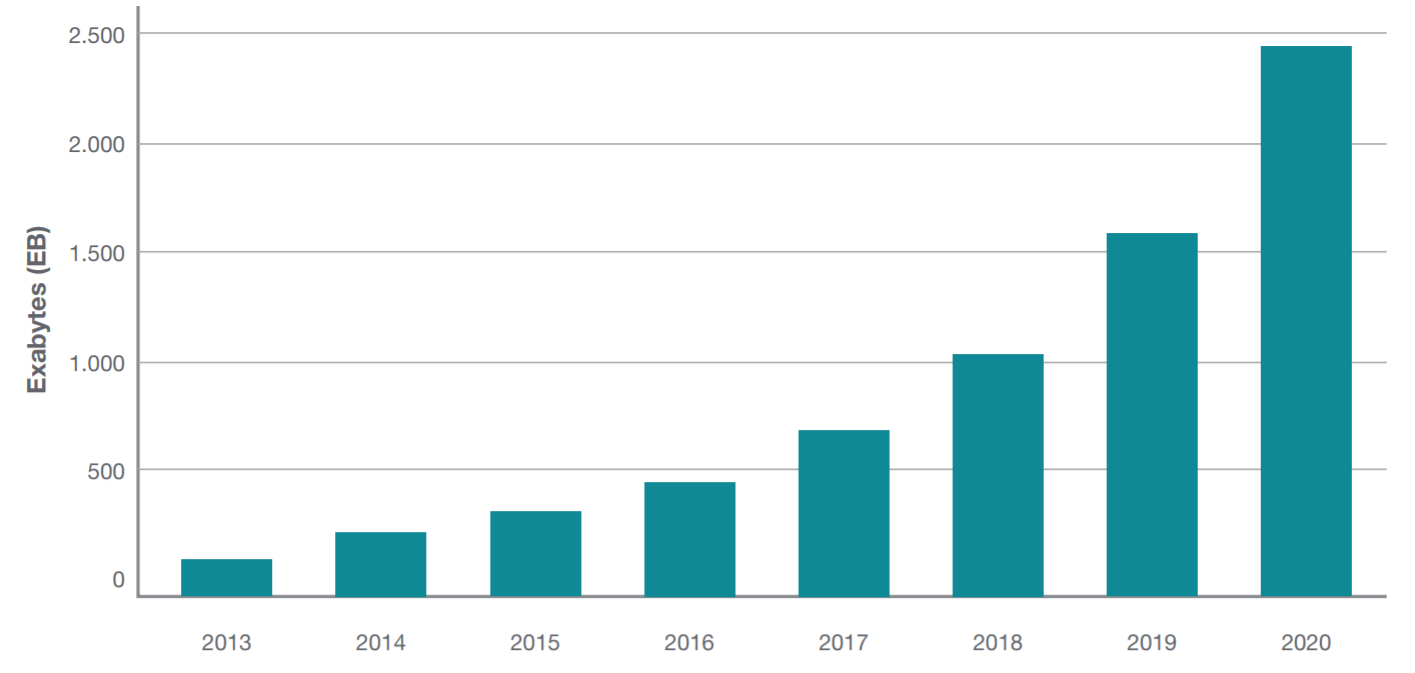
\includegraphics[scale=0.5]{TemplateTesi/immagini/healthcare-data-growth.png}
    
    \caption{Quantità di dati clinici prodotti annualmente dal 2013 al 2020 \cite{crescitadaticlinici}}
    \label{fig:my_label}
\end{figure}
%
%\section{Dati Sintetici Clinici}
%%In ambito medico, l'uso dei dati sintetici, definiti come dati generati a partire da dati reali che mantengono le stesse proprietà statistiche, è fondamentale per affrontare le sfide legate alla privacy e alla sicurezza dei dati sensibili dei pazienti. L'obiettivo principale nell'utilizzo dei dati sintetici è garantire la "utility" dei dati generati, ovvero la misura con cui questi dati sintetici mantengono la somiglianza con i dati reali.\newline
\begin{flushleft}
%%L'accesso ai dati, soprattutto in Europa, può essere spesso problematico a causa delle stringenti politiche sulla privacy e dei costi associati alla raccolta dei dati. 
%%Il processo di raccolta dei dati reali può essere oneroso, limitando la disponibilità di dati completi o utilizzabili.
%%%Questa sfida evidenzia l'importanza dei dati sintetici come alternativa, in quanto consentono di superare le restrizioni legate alla raccolta e all'accesso ai dati reali, fornendo una risorsa preziosa per l'analisi e la ricerca. Questo consente agli scienziati e ai ricercatori di esplorare diversi scenari senza dover accedere direttamente ai dati reali dei pazienti, il tutto senza compromettere la riservatezza dei pazienti. 
%%%Ciò apre nuove opportunità per studiare rare condizioni mediche, valutare l'efficacia di nuovi trattamenti e predire gli esiti delle terapie.



%I modelli basati su dati sintetici consentono di superare le limitazioni associate alla disponibilità di dati reali, consentendo ai ricercatori di addestrare e raffinare algoritmi di AI su dataset più ampi e diversificati. Questo porta a una maggiore precisione nelle previsioni e nelle diagnosi, migliorando l'efficacia complessiva del servizio.
%%\end{figure}



 %La generazione di dati sintetici, o \emph{sintesi}, si basa,come illustrato in  
 %Figura~\ref{fig:synthData}, sull'utilizzo dei dati reali come punto di partenza. 
 %Questo processo coinvolge una serie di passaggi chiave, il primo dei quali è denominato "data preparation". 
 %Durante questa fase, vengono applicate diverse tecniche, tra cui:
%\begin{itemize}
    %\item Data Cleaning: un'operazione volta a rimuovere eventuali errori o inconsistenze presenti nei dati reali
%\item Data Standardization: un processo che mira a organizzare i dati secondo gli stessi schemi di formattazione e struttura
    %\item Data Harmonization: un'attività che si occupa di uniformare i dati provenienti da fonti diverse, allineandoli sotto la stessa categoria

%\end{itemize}

%Una volta completate queste operazioni di preparazione dei dati, si procede alla fase di "Data Synthesis", in cui i dati sintetici vengono generati come risultato finale del processo. 



\end{flushleft}



\section{eHealth: Motivazioni e Campi di utilizzo}
Nell'ambito dell'eHealth, che si riferisce all'utilizzo dell'informatica e della telecomunicazione nel campo della salute,
è fondamentale comprendere il motivo per cui gli sviluppi nel campo delle AI nel settore medico stiano raggiungendo risultati così promettenti,dobbiamo quindi porci le  seguenti domande chiave: 
\begin{itemize}
    \item Perché queste tecnologie sono così importanti nell'healthcare ?
    \item Quali sono le macro aree di applicazione delle AI nel settore medico?
\end{itemize}  
Nelle sezioni sottostanti proverò a dare delle risposte a questi quesiti.


\subsection{Motivazioni}

\begin{itemize}
    \item \textbf{Managing del tempo dello staff medico:}

    Nel campo della sanità, una gestione più efficace del tempo non solo offre un maggiore respiro al personale medico, consentendo loro di concentrarsi su attività di maggior valore, ma contribuisce anche a stabilire un rapporto più forte tra medico e paziente. Diversi studi\cite{RelazionePazienteDoc1}\cite{RelazionePazienteDoc2} hanno dimostrato che una comunicazione migliore e un'attenzione personalizzata da parte del personale medico possono portare a numerosi benefici sulla qualità della cura sottoposta.
    Uno studio rilevante\cite{TempoMedici} sull'impiego del tempo del personale medico ha evidenziato che, il 40\% del loro tempo viene trascorso nella sala dei medici, mentre solo il 14.7\% del tempo è dedicato all'interazione diretta con i pazienti. In questo contesto, l'impiego delle intelligenze artificiali nel managing del tempo dello staff medico assume un ruolo fondamentale. Attraverso l'adozione di soluzioni basate sull'AI, è possibile ridurre i tempi di attesa dei pazienti, ottimizzare la pianificazione delle visite e dei trattamenti, nonché garantire che il personale medico abbia il tempo adeguato per interagire con i pazienti in modo più empatico e approfondito.
    Un esempio in tale campo si può osservare nel progetto appartenente a Dedalus chiamato Clinical Management System (CMS).
    Anche grazie alle AI il sistema CMS è capace di facilitare il managing di reparti chirurgici, accellerando i tempi di attesa, migliorando le qualità delle cure e alleggerendo il carico dello staff medico.\cite{CMSDedalus}
    \newline
    \newline
    \item \textbf{Monitoring da remoto del paziente:}

     Il monitoraggio dei dati in tempo reale nei pazienti riveste un ruolo di fondamentale importanza per la valutazione continua delle condizioni di salute, il rilevamento precoce di eventuali anomalie e la personalizzazione dei trattamenti. In questo contesto, l'impiego delle intelligenze artificiali rappresenta un elemento di grande rilevanza per garantire un monitoraggio accurato e tempestivo dei pazienti\cite{MonitorAI}.
     Grazie alla capacità di elaborare in modo rapido e accurato i dati provenienti da diverse fonti, come sensori indossabili, dispositivi di monitoraggio elettronico e registrazioni cliniche, le AI possono generare modelli predittivi e algoritmi di apprendimento automatico che permettono di adattare i protocolli terapeutici in tempo reale, ottimizzando i risultati clinici e la gestione delle risorse sanitarie,casistica in cui ricade il lavoro che ho svolto presso Dedalus.
     
    \item \textbf{Offrire una nuova prospettiva:} 

    Nel settore clinico le AI sono in grado di superare le limitazioni della visione umana e offrire una prospettiva più ampia. 
    Mentre un medico si basa principalmente sui suoi studi e sull'esperienza personale per formulare diagnosi e piani di trattamento, l'AI può analizzare una vasta quantità di dati provenienti da diverse fonti, inclusi dati clinici, storici dei pazienti, risultati di test di laboratorio e letteratura medica.

    La visione di un medico è intrinsecamente limitata dal tempo a disposizione per studiare e approfondire ogni aspetto della medicina. Tuttavia, le intelligenze artificiali non sono soggette a queste restrizioni e possono elaborare enormi quantità di dati in tempi molto più brevi.
    
    L'AI può supportare i medici nella diagnosi precoce di malattie \cite{articolo1_retinopatia}, fornendo suggerimenti basati su evidenze scientifiche e confrontando i dati dei pazienti con casi simili presenti nella letteratura medica. Questo permette di evitare errori diagnostici e migliorare l'accuratezza delle diagnosi, facendo risparmiare alle strutture sanitarie risorse impiegabili per migliorare la qualità dei loro servizi.
    \item \textbf{Spinta al raccoglimento dei dati e alla digitalizzazione:}

    Le AI offrono un'opportunità per migliorare la gestione dei dati clinici, consentendo la raccolta, l'elaborazione e l'analisi efficiente di enormi quantità di informazioni.

    L'adozione delle AI promuove la digitalizzazione delle pratiche sanitarie. L'implementazione di registri elettronici dei pazienti, sistemi di prescrizione elettronica e piattaforme di telemedicina consente una gestione più efficiente dei dati e una migliore comunicazione tra  sanitari. 

    La digitalizzazione dei dati nel settore clinico ha numerosi vantaggi. Permette un accesso rapido alle informazioni, riduce gli errori di trascrizione, facilita la condivisione sicura dei dati tra diversi operatori sanitari e favorisce la collaborazione interdisciplinare. Inoltre, l'elaborazione automatizzata dei dati consente l'identificazione di pattern e correlazioni che possono contribuire a una migliore comprensione delle malattie e dei trattamenti più efficaci.
\end{itemize}

\subsection{Campi di Utilizzo}

\begin{itemize}
    \item \textbf{Personalizzazione delle cure:}

    
    le AI possono analizzare e interpretare informazioni dettagliate sui pazienti, come il loro background medico, le condizioni di salute preesistenti, i risultati dei test di laboratorio e i dati genetici.
    Sono quindi in grado di identificare pattern e correlazioni tra i dati, consentendo ai medici di prendere decisioni basate su informazioni più accurate e specifiche per ogni paziente. Questo approccio personalizzato può portare a numerosi vantaggi, come la selezione ottimale di terapie e trattamenti, la prevenzione di reazioni avverse ai farmaci e la riduzione degli errori diagnostici.
    \item \textbf{Diagnosi e Terapia:}

    
     La capacità di elaborare grandi quantità di informazioni cliniche, comprese anamnesi, esami di laboratorio, immagini diagnostiche e dati genetici permettono l'individuazione dei pattern, correlazioni e anomalie nei dati, fornendo così un supporto prezioso ai medici nel processo di diagnosi e di scelta della terapia. Questo può tradursi in una maggiore precisione e tempestività nella rilevazione e cura di malattie , consentendo un trattamento più tempestivo e mirato.
     
    \item \textbf{Quotidianità dell'ospedale per automatizzazione delle task di routine:}

     Le AI possono essere impiegate per svolgere una serie di compiti ripetitivi e di routine, consentendo al personale sanitario di concentrarsi su attività di maggiore rilievo. 
     Ad esempio, le AI possono essere utilizzate per  la pianificazione delle risorse, l'allocazione del personale e la gestione delle liste d'attesa, ottimizzando i tempi di attesa e migliorando la distribuzione delle risorse all'interno della struttura sanitaria oppure possono supportare il monitoraggio dei pazienti in tempo reale, rilevando anomalie e avvisando il personale sanitario in caso di emergenze.

\end{itemize}

 
\subsection{AI in ambito Cardiovascolare}
Come precedentemente menzionato nell'introduzione, le malattie cardiovascolari costituiscono la principale causa di mortalità a livello globale. Pertanto, è fondamentale dal punto di vista scientifico concentrare i nostri sforzi, inclusi quelli nel campo dell'AI, per mitigare l'impatto di tali patologie sul benessere umano. Di seguito saranno presentati diversi esempi di applicazioni dell'intelligenza artificiale, in particolare il ML, la computer vision(CV) e il deep learning(DL), che contribuiscono in maniera efficace ad affrontare questa sfida.
\begin{itemize}
    \item \textbf{Quantificazione dei rischi in ambito cardiovascolare attraverso tecniche e modelli predittivi: }
    
    L'imaging non invasivo cardiovascolare si presta a soluzioni moderne basate sull'AI. Come illustrato %nel seguente articolo 
    in \cite{CVDex1}, è stato possibile utilizzare tecniche di AI per quantificare il rischio cardiovascolare attraverso due metodi principali: 
    \begin{itemize}
        \item attraverso l'applicazione diretta di algoritmi di DL ai dati di immagine per la quantificazione automatica di biomarcatori prognostici
        \item attraverso l'integrazione di metriche di imaging convenzionali o basate sull'AI con dati tabellari in modelli di ML per la previsione personalizzata degli esiti.
    \end{itemize}
    \item \textbf{Identificazione dei fattori di rischio di riammissione a 30 giorni e di mortalità ospedaliera a 180 giorni per cardiopatia ischemica (CI):} 
    
    Come mostrato nello studio \cite{AIcardio2}, grazie all'uso di modelli gradient boosting regressors è stato possibile individuare tali fattori di rischio in 346.390 cartelle cliniche di casi incidenti di CI, permettendo agli operatori sanitari di migliorare l'assistenza fornita ai pazienti affetti da CI. 

    \item \textbf{Previsione di 6 esiti cardiovascolari diversi rispetto ai situazioni cliniche cardiovascolare standard:}

    
    In %tale articolo 
    \cite{AIcardio3} si mostra come è stato utilizzato il dataset MESA (Multi-Ethnic Study of Atherosclerosis) per prevedere gli esiti cardiovascolari su un periodo di 12 anni su 6.814 partecipanti di diverse etnie, di età compresa tra 45 e 84 anni, provenienti da 6 centri negli Stati Uniti. Sono stati raccolti 735 variabili da immagini, test non invasivi, questionari e pannelli di biomarcatori. Utilizzando la tecnica random survival forests, sono stati identificati i 20 migliori predittori per ciascun esito.
    Meritano menzione le seguenti features:
    \begin{itemize}
        \item Età
        \item Livelli di glucosio a digiuno 
        \item Misure dell'ecografia carotidea
        \item Punteggio collegato alla presenza di calcio dell'arteria coronarica
    \end{itemize}

    \item \textbf{Ausilio nella diagnosi di CVD:}

    In %Nel seguente articolo 
    \cite{AIcardio4} si evidenzia come, per problematiche quali l'insufficienza cardiaca, gli algoritmi di AI possano migliorare le capacità diagnostiche e il processo decisionale clinico attraverso misurazioni cardiache automatizzate. 
\end{itemize}
\section{Explainable AI (XAI) in Medicina, Chiarezza come Soluzione }

\subsection{Problema del blackbox in medicina}

Riferendosi a modelli di AI complessi, il termine "black box" rappresenta la difficoltà di comprenderne il funzionamento interno e il processo decisionale (Figura~\ref{fig:bb}). Nel settore clinico questo è particolarmente problematico poichè la trasparenza e la spiegabilità delle decisioni prese dall'AI sono di fondamentale importanza. 
I medici devono essere in grado di comprendere le ragioni dietro i risultati e le raccomandazioni fornite dai modelli per poter prendere decisioni in maniera più conscia e razionale, e valutare criticamente l'affidabilità delle previsioni generate. La mancanza di spiegabilità può ostacolare la fiducia nell'utilizzo di queste tecnologie, limitando la loro adozione nella pratica clinica\cite{trustXAI}. 


\subsection{Bias: dal mondo reale ai dati}

Il problema dei bias nelle AI rappresenta una sfida significativa che richiede attenta considerazione, specialmente nel settore clinico. 
Le AI, possono essere influenzate dai bias del mondo esterno, sia impliciti che espliciti, che possono portare a disparità nella cura. I bias possono derivare da diversi fattori, come l'eterogeneità dei dati di addestramento utilizzati, la selezione dei criteri diagnostici o la mancanza di rappresentatività delle popolazioni di pazienti. Ad esempio, se i dati di addestramento includono principalmente pazienti di una certa etnia o genere, l'AI potrebbe mostrare risultati meno accurati per pazienti di gruppi diversi \cite{MITbias}.
\begin{flushleft}

\subsection{XAI}



L'explainable AI, o XAI, rappresenta un settore del mondo delle AI che mira a rendere i modelli comprensibili e spiegabili,cercando di tamponare, o in alcuni casi risolvere, la problematiche illustrate precedentemente. 
Si tratta di un insieme di tecniche e approcci che consentono di comprendere come le decisioni vengono prese dagli algoritmi di AI.


Nel contesto medico, la XAI  consente agli operatori sanitari di comprendere il ragionamento sottostante ai risultati dell'AI. Questo è particolarmente rilevante quando si tratta di analizzare i risultati ottenuti e comprendere quali fattori influenzano la salute dei pazienti \cite{XAIdoctors}. 
Grazie alle tecniche di XAI, i medici possono identificare i contributi specifici delle features, consentendo loro di suggerire strategie più mirate per migliorare la condizione di salute del paziente ( grazie alle tecniche come SHAP e LIME). 
\begin{figure}[H]
    \centering
    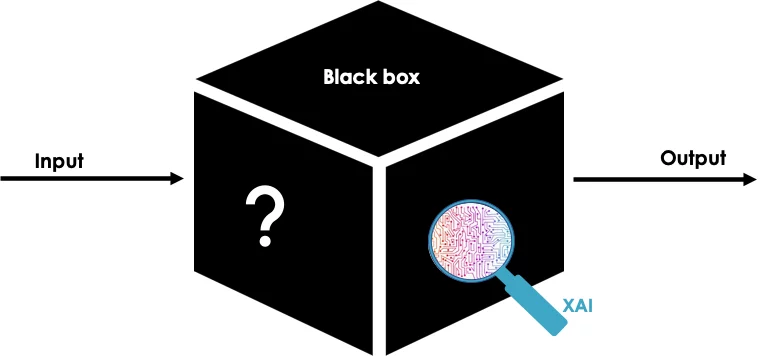
\includegraphics[scale=0.4]{TemplateTesi/immagini/blackboxpng.png}
    \caption{Problematica "Black Box" e uso della XAI \cite{imm_blackbox} }
    \label{fig:bb}
\end{figure}
Ad esempio, l'interpretazione dei modelli di AI potrebbe rivelare che determinate abitudini alimentari, personali o valori di alcune analisi influenzano significativamente la salute di un paziente. 
Queste informazioni possono aiutare i medici a consigliare cambiamenti specifici nello stile di vita, migliorando la salute complessiva dei pazienti



\end{flushleft}




\clearpage

\chapter{Machine Learning, Tecniche e Concetti}
\label{ch:capitolo2}
Questo capitolo si propone di esplorare i concetti teorici fondamentali del ML nel contesto dell'applicazione medica, con particolare attenzione alla riabilitazione dei pazienti con malattie cardiache.
% --- Inizio del Capitolo 2 ---

\section{Machine Learning, un Introduzione}
\begin{flushleft}
    

"Il Machine Learning (ML) è la branca dell'informatica che dà ai computer la capacità di apprendere senza essere  senza esser stati esplicitamente programmati."\cite{HandsOnML}
Il processo di apprendimento in ML si basa su diversi concetti fondamentali, ma tutto parte dai dati.
Essi possono essere di diversi tipi, come dati strutturati (ad esempio tabelle CSV) o non strutturati (come immagini o testo). L'obiettivo principale è quello di estrarre conoscenza e informazioni dai dati al fine di prendere decisioni o effettuare previsioni.

I dati utilizzati nel processo di apprendimento sono spesso chiamati istanze e sono caratterizzati da un insieme di features che rappresentano le loro proprietà e caratteristiche. Quando si lavora con un numero 
$n$ di features, i dati possono essere rappresentati come punti o vettori in uno spazio
$n$-dimensionale (figura \ref{fig:puntispazion}).

\begin{figure}[H]
    \centering
    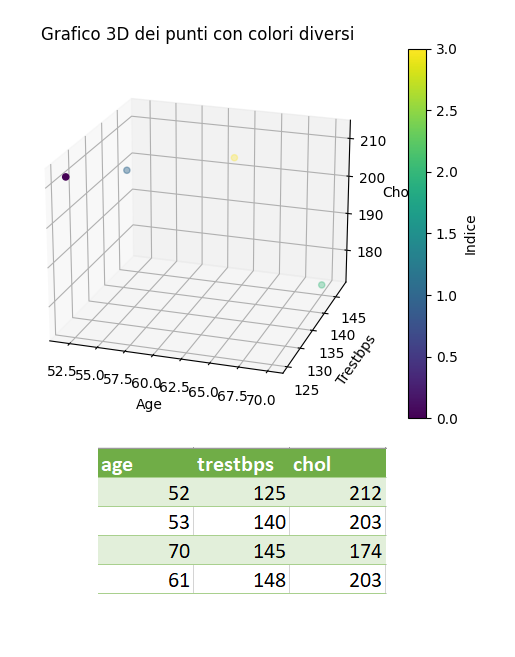
\includegraphics[scale=0.8]{TemplateTesi/immagini/tabellaplot3dbb.png}
    \caption{Da dati tabellari a Visualizzazione nello spazio}
    \label{fig:puntispazion}
\end{figure}



A seconda dell'obiettivo dell'apprendimento e della tipologia dei dati disponibili, possiamo distinguere tra:
metodi di \textbf{apprendimento supervisionato} e metodi di \textbf{apprendimento non supervisionato}. 
Nel caso dell'apprendimento supervisionato, i dati osservati sono associati a etichette, che possono essere valori categorici o numerici, rappresentando ciò che deve essere appreso in modo automatico. In pratica, si dispone di esempi in cui è nota l'etichetta corretta, e si cerca di costruire un modello che possa predire le etichette per nuovi dati in ingresso. 

I metodi di apprendimento non supervisionato, invece, mirano a estrarre informazioni di vario tipo da un insieme di osservazioni non etichettate. Questi metodi possono essere utilizzati, ad esempio, per raggruppare i dati in base alle loro somiglianze.

\subsection{Tipologie di Problemi Affrontabili}
Il ML può essere applicato a una vasta gamma di problemi. Le tipologie principali di problemi affrontabili includono:

\subsubsection{Classificazione}
La classificazione è un problema di apprendimento supervisionato in cui l'obiettivo è assegnare un'etichetta o una categoria a un'istanza di dati sulla base delle sue caratteristiche.
La classificazione  si dice \emph{binaria} se le classi di output sono esattamente due, come 0 e 1, \emph{multiclasse} altrimenti.
Ad esempio, in medicina, può essere utilizzato per classificare i tumori come benigni o maligni in base alle loro caratteristiche diagnostiche.

\begin{figure}[H]
    \centering
    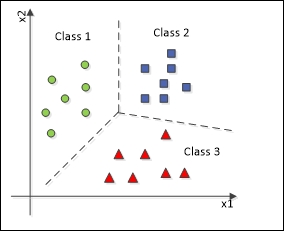
\includegraphics[scale=0.8]{TemplateTesi/immagini/B04971_06_01.jpg}
    \caption{Esempio di Classificazione multiclasse \cite{ImmClassificazione}}
    \label{fig:my_label}
\end{figure}

\subsubsection{Regressione}

La regressione si occupa di stimare o predire un valore numerico continuo sulla base delle variabili in input. 
L’obiettivo della regressione diventa dunque quello di realizzare un modello matematico che sia in grado di rappresentare una correlazione tra le features disponibili dell’input e quello che invece è il valore atteso. Questo tipo di problema è comunemente utilizzato in ambito clinico per determinare la relazione tra  diversi fattori e gli esiti delle malattie, o per identificare fattori prognostici rilevanti.\cite{Regressione}
Anche in questo caso è una tipologia di problema che risiede tra quelli di apprendimento supervisionato.
\begin{figure}[H]
    \centering
    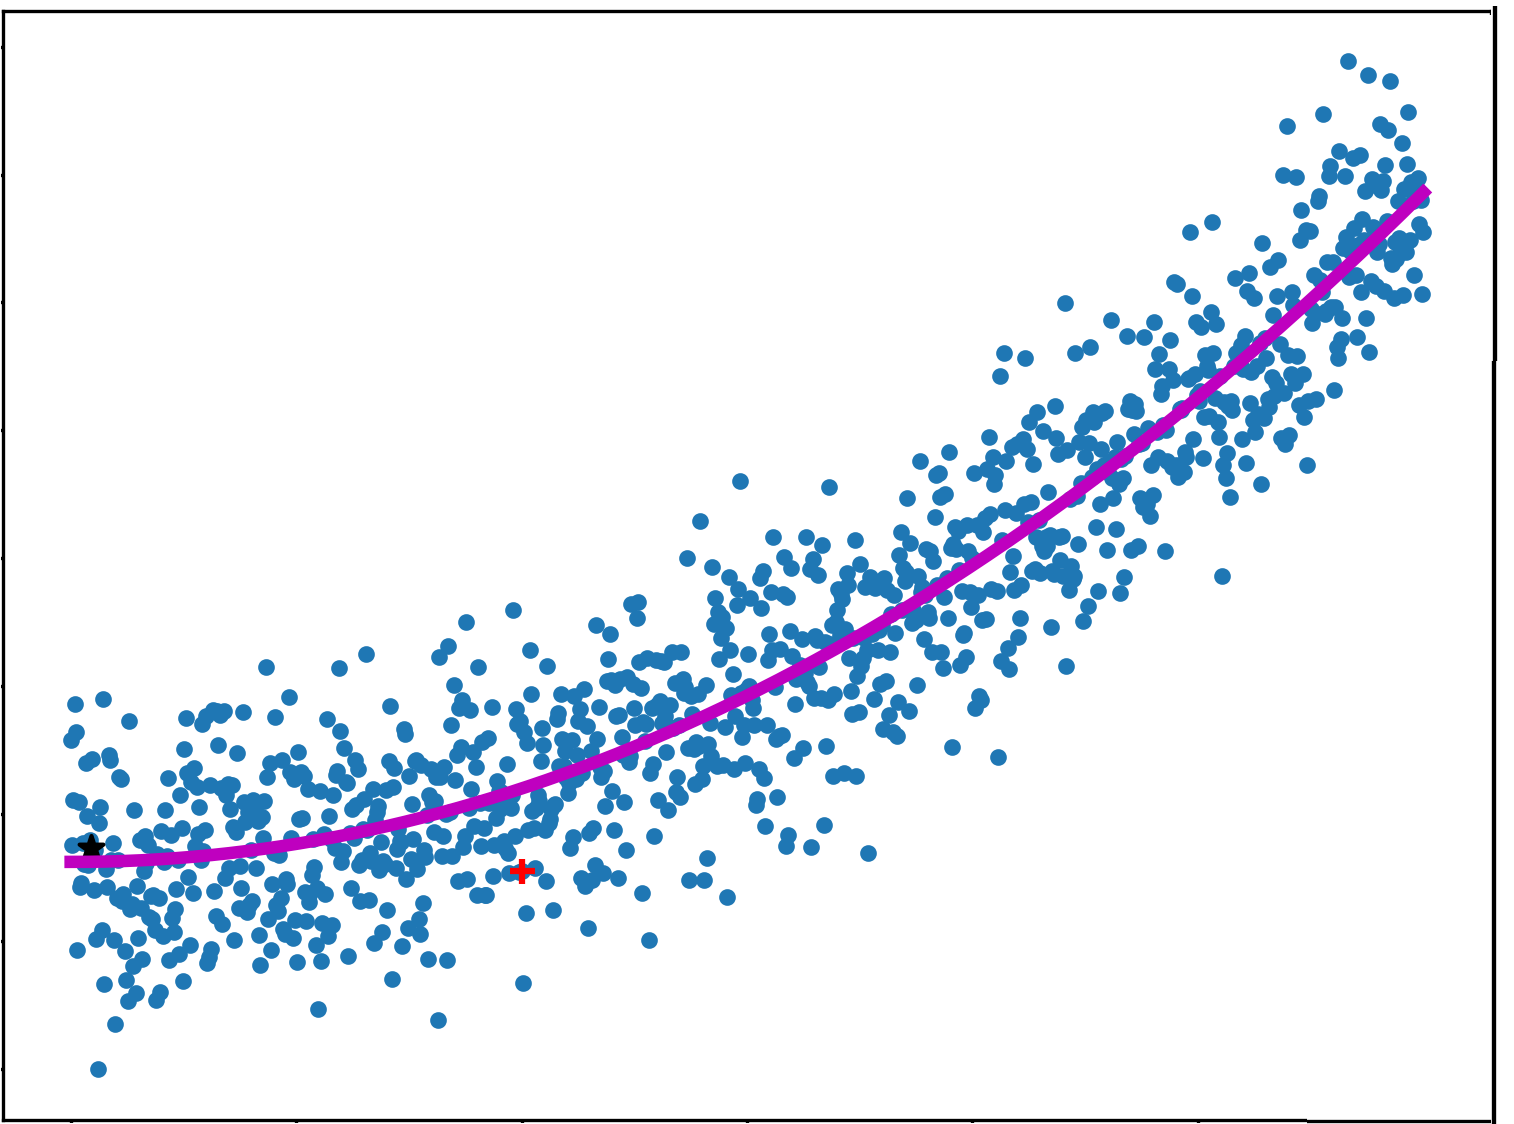
\includegraphics[scale=0.15]{TemplateTesi/immagini/TCH45-06 (1).png}
    \caption{Esempio di Regressione \cite{ImmRegressione}}
    \label{fig:my_label}
\end{figure}

\subsubsection{Clustering}

Il clustering consiste nel raggruppare gli oggetti in base alle loro somiglianze. Questo approccio può essere utilizzato per identificare sottogruppi di pazienti con caratteristiche comuni.
A differenza delle problematiche sopra descritte il clustering si basa su un apprendimento \emph{non} supervisionato.


\begin{figure}[H]
    \centering
    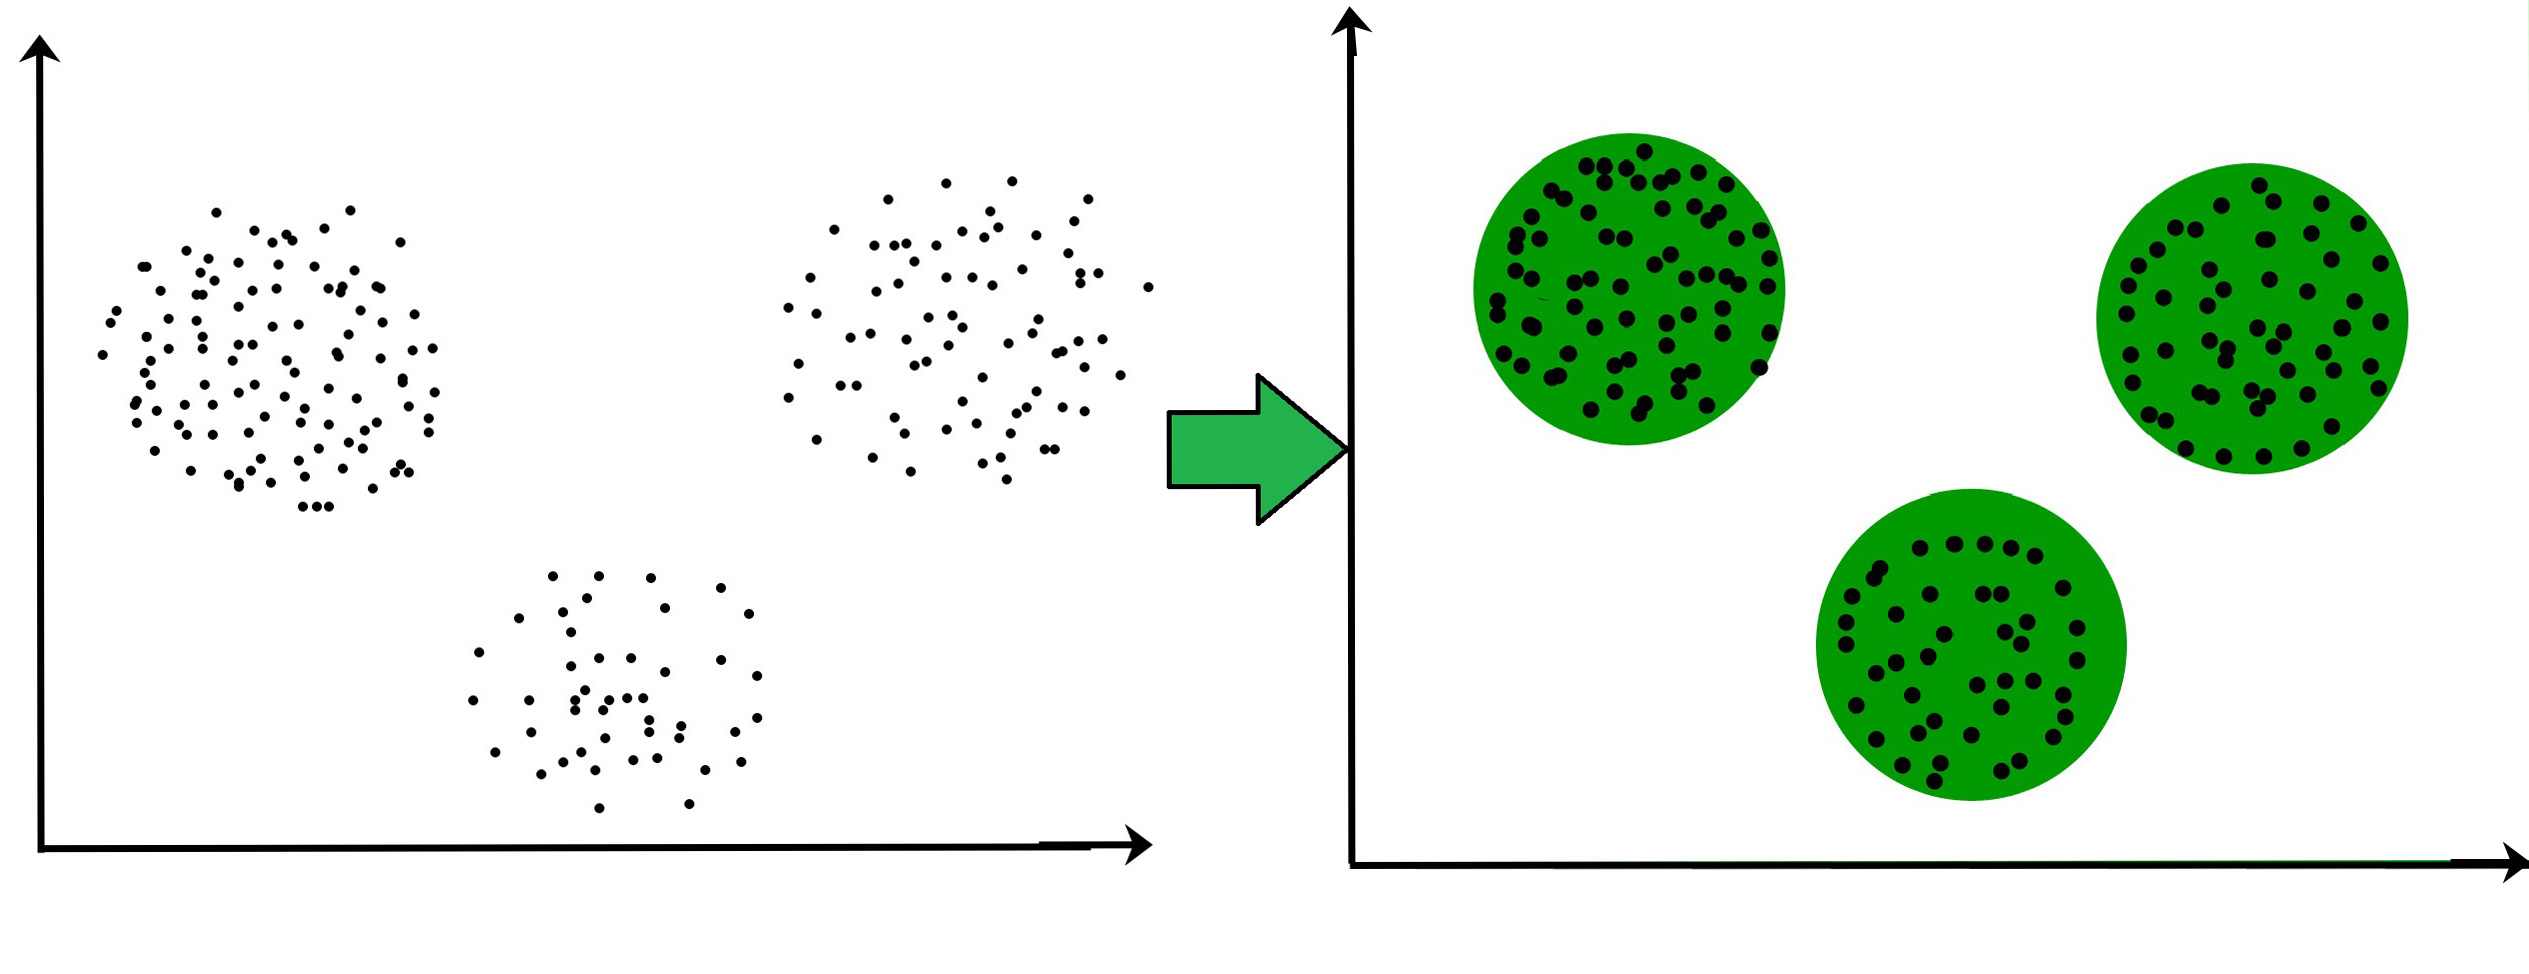
\includegraphics[scale=0.4]{TemplateTesi/immagini/merge3cluster.jpg}
    \caption{Esempio di Clustering \cite{ImmClustering}}
    \label{fig:my_label}
\end{figure}

\begin{figure}[H]
    \centering
    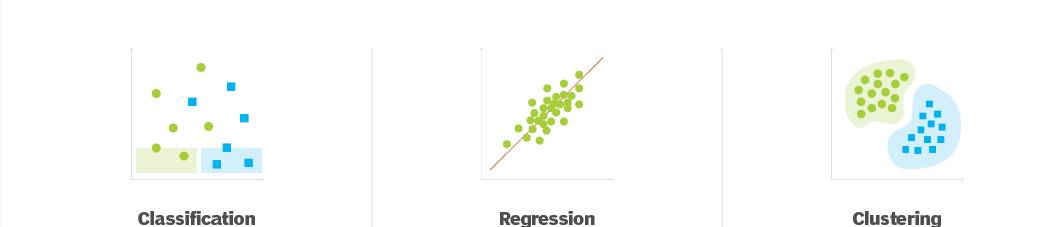
\includegraphics[scale=0.6]{TemplateTesi/immagini/businessanalytics-leading_data_science_techniques-fcut.png}
    \caption{Tipologie principali di problemi in ML \cite{ImmProblemiML}}
    \label{fig:my_label}
\end{figure}
\end{flushleft}

\section{Problematiche tipiche nel Machine Learning}
Il ML non è esente da problematiche. In questa sezione, esamineremo le principali sfide associate all'uso del ML, quali sbilanciamento delle classi, gli outlier, il continuo adattamento del modello e il bias nei dati.

\subsection{Sbilanciamento}
\begin{flushleft}
    
Nella maggior parte dei casi reali, i dataset utilizzati per addestrare i modelli di ML possono essere sbilanciati. Ciò significa che una classe di interesse può essere rappresentata da un numero significativamente inferiore di esempi rispetto ad altre classi. Lo sbilanciamento dei dati può portare a problemi nella fase di addestramento, poiché i modelli tendono ad essere influenzati dalle classi più numerose, ignorando le classi minoritarie, portando a previsioni inaccurate e a scarsa generalizzazione.

Per risolvere questa problematica possiamo attuare due approcci principali: \emph{oversampling} della classe minoritaria e \emph{undersampling} della classe maggioritaria. 

\subsubsection{Oversampling}
\begin{figure}[H]
    \centering
    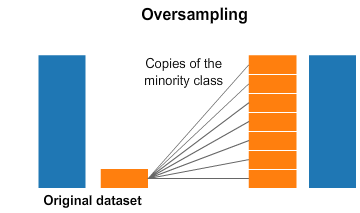
\includegraphics[scale=0.6]{TemplateTesi/immagini/oversamp.png}
    \caption{Oversampling in Dataset sbilanciato \cite{ImmOverUnderSampling}}
    \label{fig:my_label}
\end{figure}
L'oversampling è una tecnica di bilanciamento del dataset in cui le istanze della classe minoritaria vengono duplicate o generate sinteticamente per aumentare la loro frequenza nel dataset di addestramento.
Un algoritmo che implementa tale tecnica è lo \emph{SMOTE} (Synthetic Minority Oversampling Technique), questo genera nuovi campioni sintetici della classe minoritaria attraverso l'interpolazione tra i campioni di minoranza esistenti.
Il processo di interpolazione viene effettuato creando nuovi campioni sintetici lungo le linee che collegano i campioni di minoranza vicini (figura \ref{fig:smote}).


\begin{figure}[H]
    \centering
    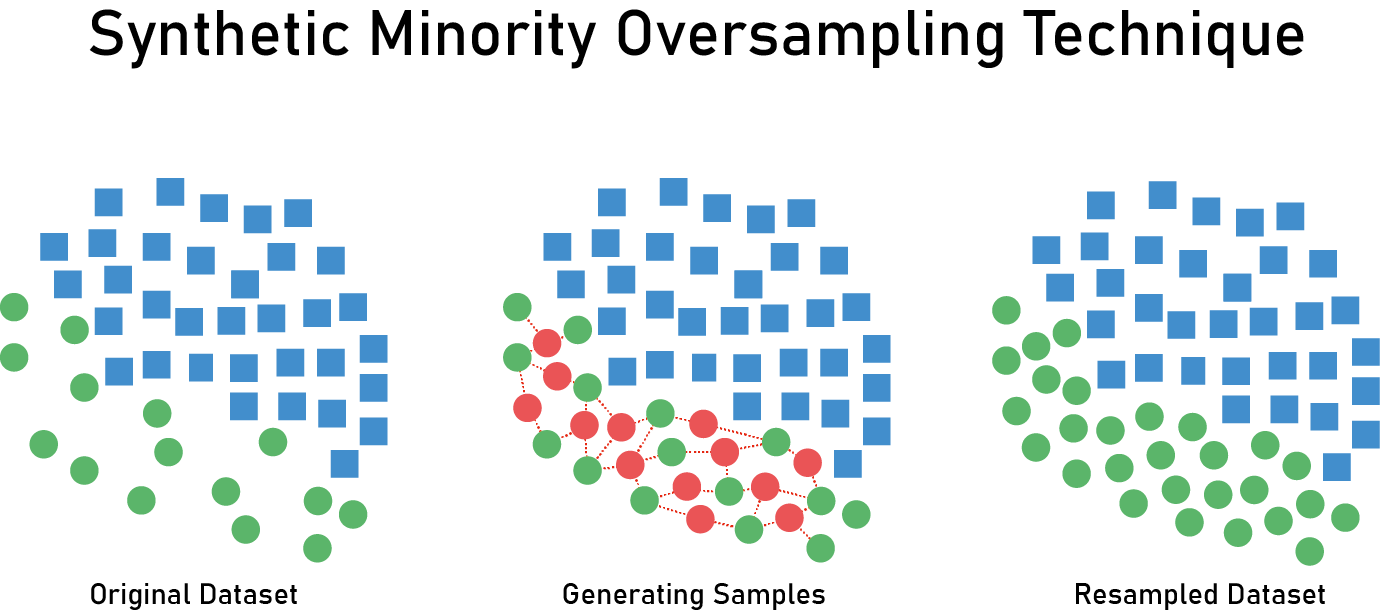
\includegraphics[scale=0.2]{TemplateTesi/immagini/smote.png}
    \caption{Funzionamento dello SMOTE}
    \label{fig:smote}
\end{figure}

\subsubsection{Undersampling}

\begin{figure}[H]
    \centering
    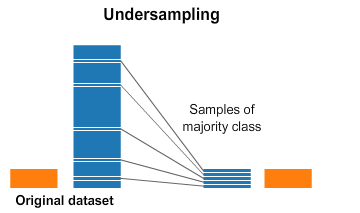
\includegraphics[scale=0.6]{TemplateTesi/immagini/undersamp.png}
    \caption{Undersampling in Dataset sbilanciato  \cite{ImmOverUnderSampling}}
    \label{fig:my_label}
\end{figure}
L'undersampling è una tecnica di bilanciamento del dataset in cui le istanze della classe maggioritaria vengono rimosse per ridurre la loro frequenza nel dataset di addestramento.
Gli algoritmi che ho valutato per la gestione dell'undersampling sono il \emph{Tomek Link} e l'\emph{ENN (Edited Nearest Neighbour)}.
Il Tomek Link (figura \ref{fig:tomek}) identifica le coppie di istanze che appartengono a classi diverse che sono molto vicine tra loro, rimuovendo il record della classe maggioritaria dal dataset di training.
L'ENN invece seleziona un insieme di K punti della classe minoritaria e l'insieme dei punti della classe maggioritaria più vicini ad essi\ref{fig:enn}),rimuovendo i suddetti punti della classe maggioritaria.
In entrambi i casi riduciamo la sovrapposizione tra le classi aumentando la distanza tra le istanze, migliorando la capacità del modello di distinguere tra le classi.
È bene tenere di conto però che parametri di selezione troppo stringenti possono portare ad una perdita di informazione e conseguentemente una precisione minore da parte del modello.

\begin{figure}[H]
    \centering
    
\includegraphics[scale=0.4]{TemplateTesi/immagini/tomek.png}
    \caption{Funzionamento del Tomek Link \cite{ImmTOmekLink}}
    \label{fig:tomek}
\end{figure}


\begin{figure}[H]   
    \centering
    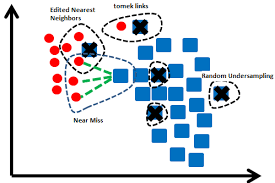
\includegraphics[scale=0.7]{TemplateTesi/immagini/enn.png}
    \caption{Funzionamento dell'ENN \cite{ImmENN}}
    \label{fig:enn}
\end{figure}


\subsection{Outliers}
Gli outliers sono dati che si discostano significativamente dagli altri punti della stessa distribuzione o cluster, i problemi legati ad essi sono l’identificazione e la cancellazione degli stessi

\subsubsection{Z-Score}

\begin{figure}[H]
    \centering
    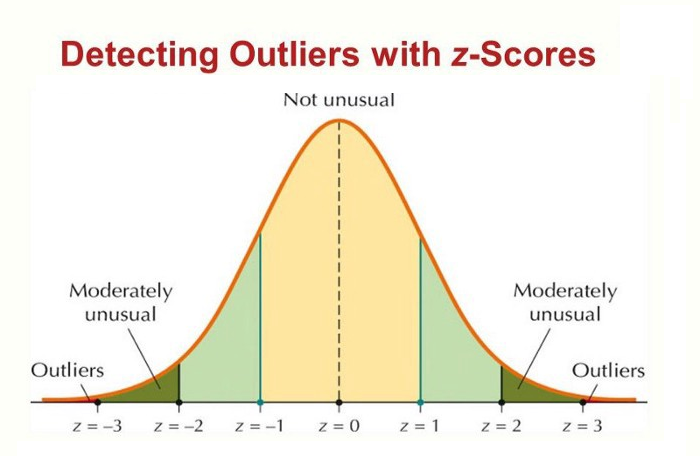
\includegraphics[scale=0.3]{TemplateTesi/immagini/Zscore.png}
    \caption{Zscore per rilevazione e cancellazione degli outlier \cite{ImmZscore}}
    \label{fig:zscore}
\end{figure}

Lo Z-score è una tecnica utilizzata per rilevare e cancellare gli outlier nei dataset, utilizza la deviazione standard e la media dei dati per identificare i valori che si discostano significativamente dalla media.
Il suo funzionamento segue la formula:

$$Z=\frac{X- \mu}{\sigma}$$
                                      
dove:
\begin{itemize}
    \item $\mu=deviazione  standard$
    \item $\sigma=media$
\end{itemize}



Una volta che avremo deciso un valore soglia "$n$" verranno eliminati tutti i punti distanti $n$ deviazioni standard dalla media.


\subsubsection{IQR Score}
L'IQR, Interquartile Range, è una misura della dispersione utilizzata per rilevare gli outlier nei dataset.
Ci basiamo sulla suddivisione in quartili della distribuzione dei dati per cancellare i valori che si discostano troppo dalla mediana.
L'outlier viene identificato come tale quando il suo valore è al di fuori di un intervallo soglia specificato.
Valori soglia standard sono di solito 1,5 oppure 3 volte la deviazione interquartile.
\begin{figure}[H]
    \centering
    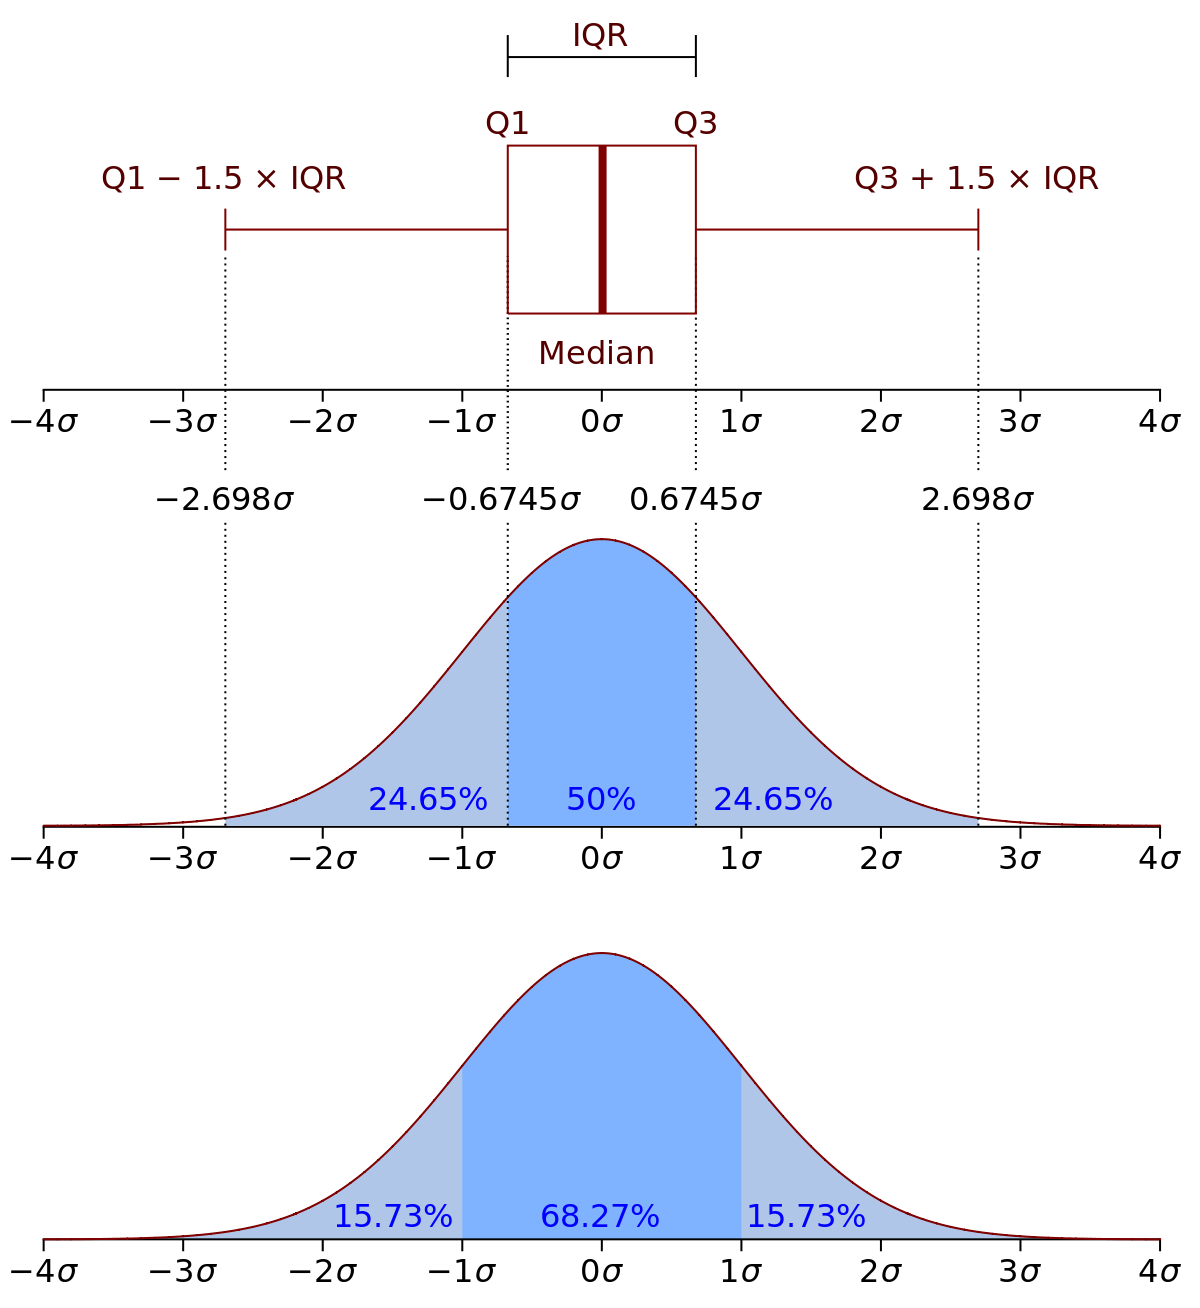
\includegraphics[scale=0.2]{TemplateTesi/immagini/iqr.png}
    \caption{IQR per rilevazione e cancellazione outlier \cite{ImmIQR}}
    \label{fig:my_label}
\end{figure}

.
\newline
L'IQR viene calcolato come:

$$IQR=Q3-Q1$$
con:
\begin{itemize}
    \item Q1= Lower Quartile 
    \item Q3= Upper Quartile
\end{itemize}





\subsection{Adattamento del Modello}

Il ML si basa sull'idea che i modelli possano apprendere dai dati e adattarsi per fare previsioni o prendere decisioni. Questo significa che il modello è rappresentato da una funzione matematica che mappa gli input ai corrispondenti output desiderati. Durante la fase di training, il modello cerca di approssimare questa funzione utilizzando un insieme di dati di addestramento.

Tuttavia, i modelli di ML possono incontrare sfide nel raggiungere un adattamento ottimale ai dati. Queste sfide possono derivare da diversi fattori, come la mancanza di rappresentatività dei dati di addestramento o la complessità del problema affrontato.


Subentrano quindi due problematiche molto frequenti ovvero:
\begin{itemize}
    \item \textbf{Overfitting}: Il modello di ML si adatta troppo ai dati di addestramento, non generalizzando bene sui nuovi dati
    \item \textbf{Underfitting}: Il modello non è in grado di adattarsi correttamente ai dati di addestramento e manca di capacità predittiva
\end{itemize}  

\begin{figure}[H]
    \centering
    
\includegraphics[scale=0.5]{TemplateTesi/immagini/fitting.png}
    \caption{Overfitting,Underfitting e fitting ottimale comparati \cite{ImmFittingComparazione}}
    \label{fig:fitting}
\end{figure}
Per affrontare questi due problemi possiamo utilizzare tecniche come la cross validation e la data augmentation:

\subsubsection{Cross Validation}
 È una tecnica ampiamente utilizzata per valutare le prestazioni di un modello di ML e affrontare il problema dell'overfitting. 
 
La cross validation (figura \ref{fig:crossvalidation}) suddivide l'insieme di dati di addestramento in K sottoinsiemi, noti come fold. Successivamente, il modello viene addestrato K volte, ogni volta utilizzando K-1 fold come dati di addestramento e il fold rimanente come dati di validazione. Questo processo di addestramento e validazione viene ripetuto K volte, in modo che ogni fold venga utilizzato almeno una volta come dati di validazione.

\begin{figure}[H]
    \centering
    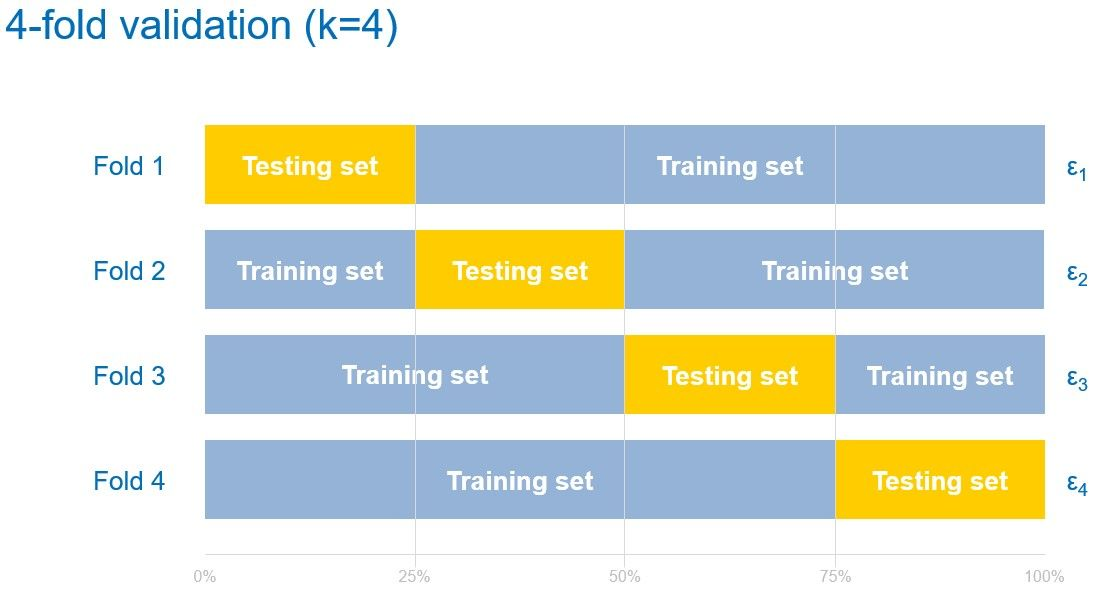
\includegraphics[scale=0.3]{TemplateTesi/immagini/kfold.jpg}
    \caption{Funzionamento della Cross Validation \cite{ImmKFOld}}
    \label{fig:crossvalidation}
\end{figure}
\subsubsection{Data Augmentation}
 Il training dei modelli può richiedere una grande quantità di dati di addestramento. 
 Tuttavia, in molte applicazioni, può essere difficile raccogliere o etichettare un numero sufficiente di dati. 
 La data augmentation è una tecnica ampiamente utilizzata per affrontare questa sfida.
 Lo scopo principale della data augmentation è aumentare la quantità e la varietà dei dati di training disponibili, al fine di migliorare le prestazioni del modello.

 Tra le tecniche principali di data augmentation troviamo ad esempio:
 \begin{itemize}
     \item Noise injection: Aggiunta di un rumore gaussiano o randomico ai dati 
     \item Generative adversarial networks (GANs): Vengono usate per generare nuovi punti o nuove immagini 
     \item Trasformazioni geometriche: utilizzate per modificare la posizione e la forma dei dati nei dataframe di immagini. Queste trasformazioni includono la traslazione, la rotazione, lo scaling, la riflessione e lo zoom (figura \ref{fig:trasformazioni})
 \end{itemize}
 

\begin{figure}[H]
    \centering
    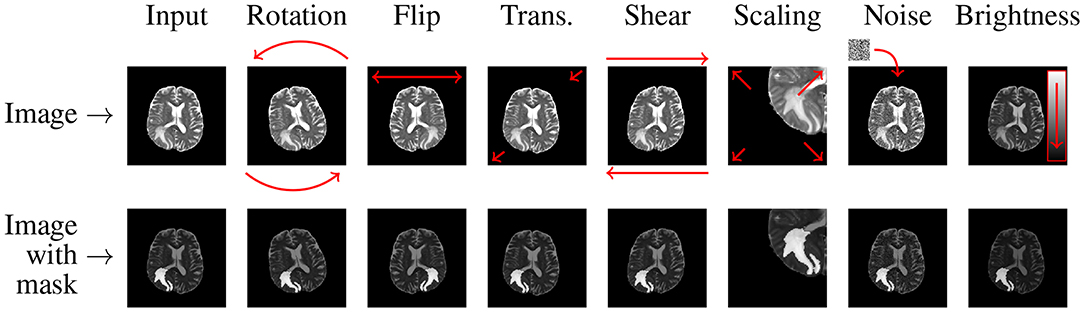
\includegraphics[scale=0.45]{TemplateTesi/immagini/fncom-13-00083-g003.jpg}
    \caption{Esempio di Data Augmentation con trasformazioni geometriche in Healthcare \cite{imm_dataaug}}
    \label{fig:trasformazioni}
\end{figure}

\subsection{Bias}
Nel contesto del ML, il termine "bias" si riferisce a una serie di problematiche che possono influenzare negativamente i modelli e le decisioni prese da essi. 
Il bias può derivare da molteplici fonti, come i dati di addestramento sbilanciati, i pregiudizi umani incorporati nei dati o negli algoritmi, o le limitazioni dei modelli stessi.
Tra le varie tipologie di bias troviamo\cite{biasgoogle}:
\begin{itemize}
    \item Reporting Bias:  si verificano quando la frequenza di eventi, o esiti catturati in un dataset non riflette accuratamente la loro frequenza nel mondo reale.
    \item Automation Bias: tendenza a favorire i risultati generati da sistemi automatizzati rispetto a quelli generati da sistemi non automatizzati,come l'ispezione da parte di un lavoratore, indipendentemente dai tassi di errore di ciascuna delle parti.
    \item Implicit Bias: si verificano quando si fanno ipotesi basate sui propri preconcetti e sulle proprie esperienze personali che non si applicano necessariamente al mondo reale.
    \begin{itemize}
        \item Confirmation Bias: Bias dove chi costruisce il modello elabora inconsciamente i dati in modo da affermare convinzioni e ipotesi preesistenti
        \item Experimenter's Bias: Bias per cui chi addestra il modello continua fino a quando non produce un risultato che si allinea con la sua ipotesi iniziale 
    \end{itemize}
\end{itemize}

L'Explainable AI accennata nel capitolo precedente( che verrà ulteriormente trattata in questo capitolo) è una valida soluzione per mitigare o comprendere i bias presenti nel nostro modello.  

\section{Metriche di Valutazione}


Nel contesto dell'analisi delle prestazioni dei modelli di ML per la classificazione binaria, è di fondamentale importanza avere una chiara comprensione dei concetti di true positive (TP), true negative (TN), false positive (FP) e false negative (FN). Questi concetti 
offrono una panoramica delle capacità predittive di un modello.

\begin{itemize}
    \item \textbf{True Positive}: si verifica quando il modello classifica correttamente un'istanza come positiva, corrispondente alla sua reale etichetta positiva.
    \item \textbf{True Negative}: il modello classifica correttamente un'istanza come negativa, in accordo con la sua reale etichetta negativa. Rappresenta il caso in cui il modello riconosce correttamente l'assenza di una condizione positiva

\item \textbf{False Positive}:  il modello classifica erroneamente un'istanza come positiva, nonostante la sua reale etichetta sia negativa. Indica un falso allarme, in cui il modello indica erroneamente la presenza di una condizione positiva quando non è effettivamente presente. 

\item \textbf{False Negative}: il modello classifica erroneamente un'istanza come negativa, nonostante la sua reale etichetta sia positiva. Questo rappresenta un errore di mancata identificazione di una condizione positiva
\end{itemize}
Ad esempio:
\begin{itemize}
    \item True Positive: nella diagnosi di una malattia, un true positive si verifica quando il modello identifica correttamente un paziente come affetto dalla malattia e il paziente  ne è effettivamente affetto. 
    \item True Negative: nella classificazione di email come spam o non spam, un true negative si verifica quando il modello correttamente identifica un'email come non spam e l'email effettivamente non è spam.
    \item False Positive:  nella diagnosi di una malattia, un false positive si verifica quando il modello indica erroneamente che un paziente è affetto dalla malattia, ma il paziente non ne è affetto
    \item False Negative: nella classificazione di email , come prima, un false negative si verifica quando il modello non riesce a riconoscere un'email come spam, nonostante l'email sia effettivamente spam
\end{itemize}


\subsection{Confusion Matrix}
La Confusion Matrix è uno strumento statistico  utilizzato per valutare le prestazioni dei modelli di classificazione.
È una matrice quadrata che visualizza il numero di campioni di dati classificati correttamente e erroneamente dal modello, in base ai valori delle metriche sopra descritte.
La confusion matrix ci permette di avere una rapida visione della classificazione dei valori, la sua struttura è rappresentata in figura \ref{fig:confusionmatrix}

\begin{figure}[H]
    \centering
    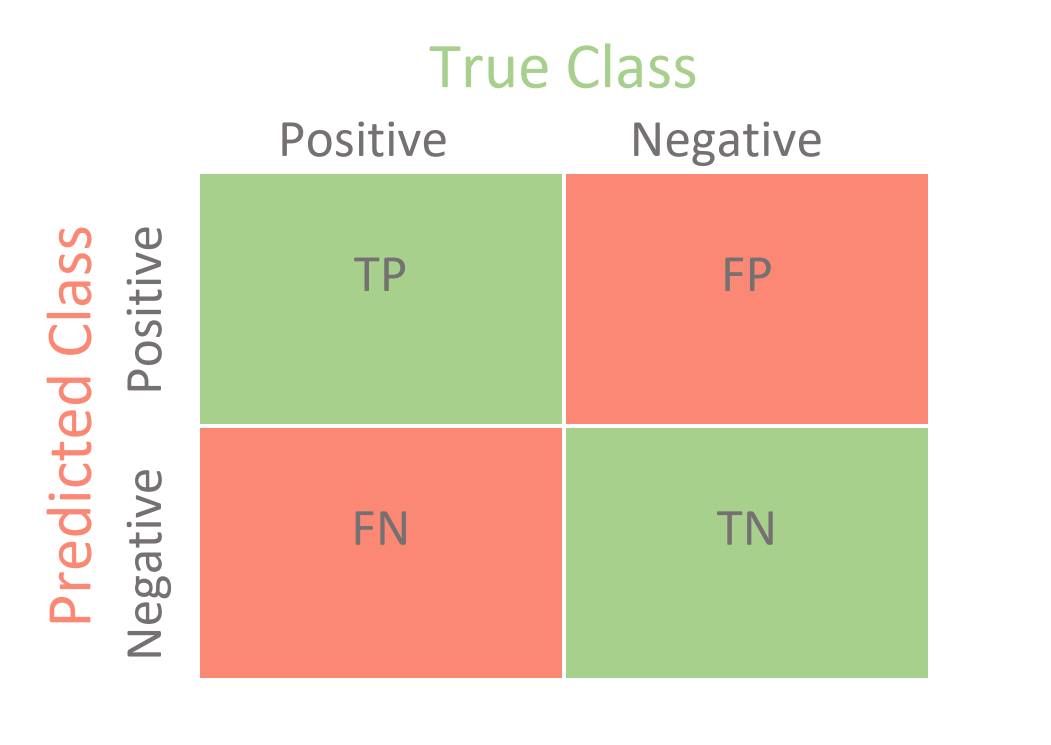
\includegraphics[width=0.5\linewidth]{TemplateTesi//immagini/confusionmatrix.png}
    \caption{Struttura della Confusion Matrix \cite{ImmConfusionMatrix}}
    \label{fig:confusionmatrix}
\end{figure}
\subsection{Accuracy, Precision e Recall}

Le metriche di valutazione nel ML, come accuracy, precision e recall, sono direttamente correlate ai concetti di true positive, true negative, false positive e false negative. Questi concetti vengono utilizzati per calcolare queste metriche e fornire una valutazione più completa delle prestazioni del modello.

Le metriche fondamentali su cui si basano anche quelle più complesse sono quindi le 3 elencate precedentemente:

\begin{itemize}
    \item \textbf{Accuracy}: Metrica che viene utilizzata per tenere traccia delle previsioni effettuate correttamente.
    Rappresenta la proporzione di campioni correttamente valutati sul totale dei campioni:
    \[\frac{Predizioni Corrette}{Predizioni Totali}\]
    o più formalmente:
    \[\frac{TP+TN}{TP+TN+FP+FN}\]
    (Non tiene traccia dei falsi negativi)
    
    \item \textbf{Recall}: Metrica che risponde alla domanda "Quale proporzione di 'Positive' è stata identificata correttamente?"
    calcolata come:

    \[\frac{TP}{TP+FN}\]
    (Non tiene traccia dei falsi positivi)


    \item \textbf{Precision}: La precision misura la percentuale di istanze positive identificate correttamente rispetto a tutte le istanze identificate come positive dal modello. In altre parole, indica quanto sia preciso il modello nel predire correttamente le istanze positive. 
    La formula per calcolare la precision è la seguente:
    \[\frac{TP}{TP+FP}\]

\end{itemize}

\section{Preprocessing}
Il preprocessing dei dati svolge un ruolo fondamentale nel ML, in questa fase risiede la preparazione dei dati per il training.
Consiste in una serie di trasformazioni e operazioni volte a rendere i dati idonei per l'apprendimento del modello. 
Nel settore dell'healthcare, il preprocessing dei dati è particolarmente cruciale, poiché i dati sanitari possono essere complessi, eterogenei e soprattutto sensibili.
Di seguito 3 procedure tipiche del preprocessing dei dati: 
\begin{itemize}
    \item \textbf{Pulizia Dati}: i dati, come anticipato, sono spesso complessi ed eterogenei.
    Possono provenire da diverse fonti, come dispositivi medici o registri elettronici. 
    Questa eterogeneità può portare a dati sporchi o incompleti, che possono influenzare negativamente l'addestramento dei modelli di ML. Pertanto, è fondamentale condurre un'attenta pulizia dei dati prima di utilizzarli per il training del modello.
    La pulizia dei dati può includere diverse attività, come la rimozione dei valori mancanti o errati, la gestione degli outlier e la standardizzazione delle variabili. Ad esempio, potrebbe essere necessario rimuovere i record dei pazienti con dati mancanti, al fine di evitare un'analisi distorta o un addestramento del modello inaccurato.
    \item \textbf{Scaling}: lo scaling dei dati è una tecnica essenziale per garantire che le variabili abbiano un impatto comparabile sul modello di ML. Lo scaling dei dati implica la trasformazione delle variabili in modo che abbiano una scala comune, riducendo così le differenze di scala tra le variabili stesse.
    tra le varie tecniche di scaling troviamo:
    \begin{itemize}
        \item Z-Score Scaling: trasforma i dati in modo che abbiano una media zero e una deviazione standard unitaria. La formula per calcolare lo Z-Score Scaling di un dato $x$ è:

        
\[x\_scaled = \frac{(x - mean)}{std}\]


        Dove "$mean$" rappresenta la media della variabile e "$std$" rappresenta la deviazione standard della variabile.

    \item Min-Max Scaling: Un'altra tecnica comune per lo scaling dei dati è il Min-Max Scaling, che trasforma i dati in un intervallo specifico, di solito compreso tra 0 e 1. La formula per calcolare il Min-Max Scaling di un dato $x$ è:

       
\[ x\_scaled = \frac{(x - min)}{max - min}\]


    Dove "$min$" rappresenta il valore minimo della variabile e "$max$" rappresenta il valore massimo della variabile. 

    \item Robust Scaling: Questa tecnica utilizza la mediana e l'intervallo interquartile (IQR) per ridimensionare i dati. La formula per calcolare la Robust Scaling di un dato $x$ è:

  
\[  x\_scaled = \frac{(x - mediana)}{IQR}\]


    Dove "$mediana$" rappresenta la mediana della variabile e "$IQR$" rappresenta l'intervallo interquartile della variabile.
    \end{itemize}
    \item \textbf{Feature Selection}:
    La feature selection è il processo di selezione delle features più rilevanti da un insieme iniziale per addestrare i modelli di ML. L'obiettivo è eliminare le caratteristiche poco informative, riducendo così la dimensione dello spazio delle caratteristiche, quindi la complessità generale del modello e migliorandone la generalizzazione. Una selezione accurata delle features può portare a modelli più semplici, che richiedono meno dati per l'addestramento e producono risultati più stabili.
\end{itemize}
\section{Modelli}
Alla base di ogni tool di AI, oltre ai dati, troviamo il modello.
Di seguito verranno illustrati vari modelli che ho tenuto in considerazione durante il mio lavoro di tesi.

\subsection{Support Vector Machine}
Le SVM (Support Vector Machine) sono un tipo di modello di apprendimento supervisionato che possono essere utilizzate per la classificazione e la regressione.
L'obiettivo delle SVM, nel contesto della classificazione, è quello di trovare un iperpiano che separi in modo ottimale i punti di dati delle diverse classi nel miglior modo possibile, dove un iperpiano è definito come un sottospazio lineare di dimensione inferiore di uno rispetto allo spazio in cui è contenuto\cite{def_iperpiano}.
\begin{figure}[H]
    \centering
    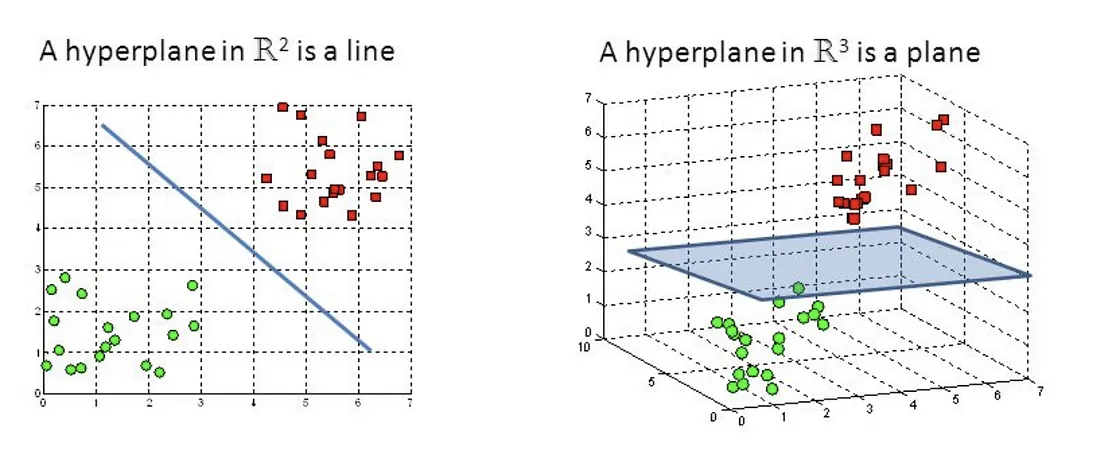
\includegraphics[width=0.7\linewidth]{TemplateTesi//immagini/1_ZpkLQf2FNfzfH4HXeMw4MQ.png}
    \caption{Esempi di Iperpiani \cite{imm_svm}}
    \label{fig:enter-label}
\end{figure}\newpage

SVM fa uso di due concetti fondamentali:

\begin{itemize}
\item \textbf{Kernel}:

     Per kernel si intende una funzione matematica che consente di mappare i dati dallo spazio delle features originale a uno spazio di dimensione superiore, dove i dati possono essere più facilmente separabili.

     L'utilizzo delle funzioni kernel è conosciuto come "kernel trick" (figura \ref{fig:kerneltrick})ed è una delle caratteristiche distintive delle SVM. La principale motivazione dietro l'utilizzo dei kernel è che, sebbene i dati nel loro spazio originale possano non essere separabili linearmente, potrebbero essere separabili in uno spazio di dimensione superiore.
    \begin{figure}[H]
        \centering
        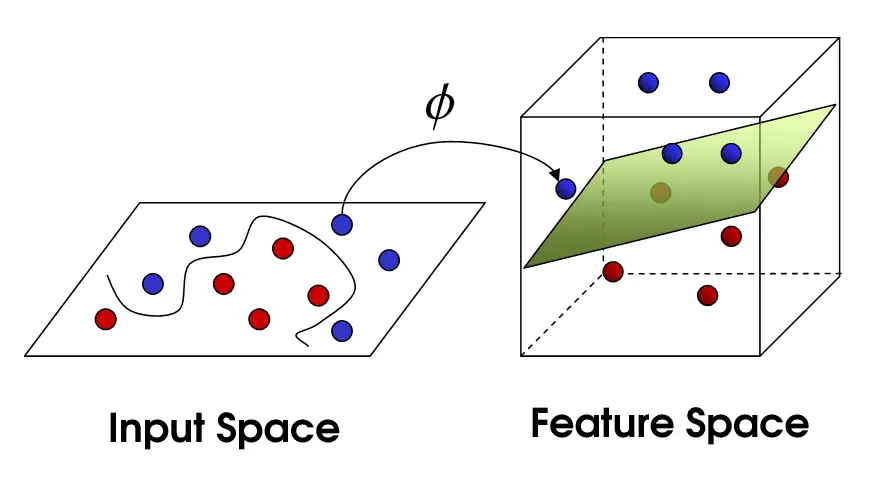
\includegraphics[width=0.6\linewidth]{TemplateTesi//immagini/1_zWzeMGyCc7KvGD9X8lwlnQ.png}
        \caption{Il Kernel Trick \cite{imm_svmkerneltrick}}
        \label{fig:kerneltrick}
    \end{figure}
    \item \textbf{Massimizzazione del Margine}:
    Il concetto di margine è fondamentale nelle Support Vector Machines e gioca un ruolo chiave nell'ottimizzazione della separazione dei dati. Il margine rappresenta la distanza tra l'iperpiano di separazione e i dati di ciascuna classe.
    L'obiettivo delle SVM quindi è quello di massimizzare il margine, poiché un margine ampio indica una migliore generalizzazione del modello e una maggiore capacità di gestire dati non visti in fase di addestramento
    \end{itemize}



\subsection{Random Forest}
Tra i modelli di ML valutati durante il mio lavoro di tesi, il Random Forest si è dimostrato il più performante. Questo modello si basa sull'utilizzo degli alberi decisionali e sfrutta il concetto di entropia per creare una foresta di alberi decisionali, con i quali effettuare le predizioni.

\subsubsection{Entropia di Shannon}
L'entropia può essere definita come una misura che quantifica il livello di disordine o incertezza presente in un sistema.
Nel contesto del ML, si traduce in un concetto derivato dalla teoria dell'informazione di Claude Shannon. Rappresenta quindi la quantità di informazione media contenuta in un insieme di dati. Maggiore è l'entropia, maggiore è l'incertezza o il disordine nell'insieme di dati.

L'entropia di un insieme $S$ con $n$ possibili classi $i$ , denotate come \(\{i_1, i_2, ..., i_n\}\), può essere quindi calcolata utilizzando la seguente formula:
$$E(S) = -\sum_{i=1}^{n} (p_i \log_2(p_i))$$

Nel contesto di utilizzo di un modello di ML il nostro obiettivo è quello di minimizzare l'entropia dei gruppi generati dal modello.

\subsubsection{Alberi Decisionali}
\begin{figure}[H]
    \centering
    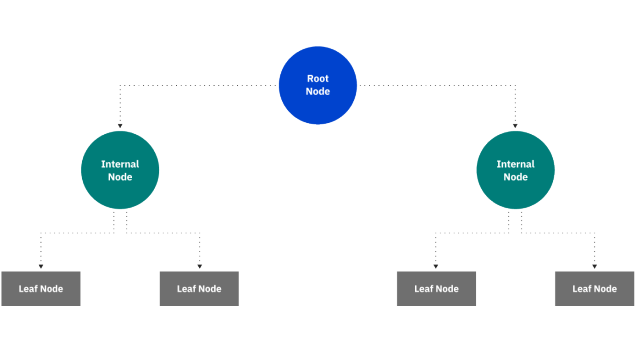
\includegraphics[width=0.7\linewidth]{TemplateTesi/immagini/alberodecibmstruttura.png}
    \caption{Struttura di un albero decisionale \cite{ibmdecisiontrees}}
    \label{fig:ibmtrees_struttura}
\end{figure}
Un albero decisionale è un algoritmo di apprendimento supervisionato, utilizzato sia per attività di classificazione che di regressione \cite{ibmdecisiontrees}. Si compone di una struttura ad albero gerarchica, che consiste di un nodo radice, di rami, nodi interni e nodi foglia (figura \ref{fig:ibmtrees_struttura}) , ogni nodo rappresenta un test su una feature e ogni ramo rappresenta il risultato di quel test, come vediamo in figura \ref{fig:ibmtrees}.

Gli alberi decisionali sono costruiti utilizzando algoritmi che cercano di dividere l'insieme di dati in sottoinsiemi omogenei. La divisione viene effettuata in modo iterativo selezionando le caratteristiche e i test che massimizzano la riduzione dell'incertezza e quindi quello che viene chiamato "Information Gain"(IG), selezionando la suddivisione che produce meno entropia nei dati.

$$IG = E(parent) - E(child)$$

\begin{figure}[H]
    \centering
    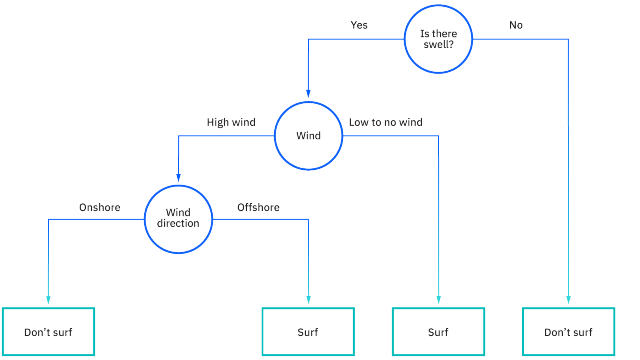
\includegraphics[width=0.7\linewidth]{TemplateTesi//immagini/alberidecisionaliibm.png}
    \caption{Funzionamento Albero Decisionale \cite{ibmdecisiontrees}}
    \label{fig:ibmtrees}
\end{figure}

\subsubsection{Creazione della Foresta}
La foresta di alberi decisionali che compongono il concetto di "Random Forest" viene creata seguendo il concetto di "ensemble learning",una tecnica che combina diversi modelli di apprendimento per ottenere prestazioni migliori rispetto al singolo modello. Nel
caso del random forest, l'ensemble è costituito da un insieme di alberi decisionali.

Per creare ciascun albero decisionale, viene utilizzato un sottoinsieme casuale dei dati di addestramento. Questa tecnica viene chiamata "bagging" (figura \ref{fig:bagging}).
Si compone partendo da due concetti chiave: il bootstrap e l'aggregazione.
\begin{figure}[H]
    \centering
    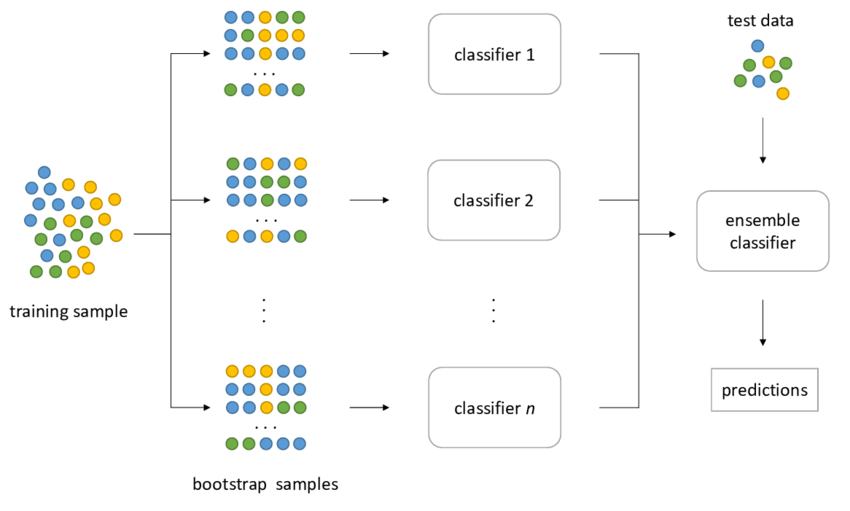
\includegraphics[width=0.8\linewidth]{TemplateTesi//immagini/bagging-1.png}
    \caption{Tecnica "Bagging" \cite{immbagging}}
    \label{fig:bagging}
\end{figure}

\begin{itemize}
    \item \textbf{Il Bootstrap} è un metodo di campionamento che prevede la selezione casuale di campioni dall'insieme di dati di training, consentendo la possibilità che un campione venga selezionato più volte o non venga selezionato affatto. Questo processo di selezione ci permette di creare diversi sottoinsiemi di dati a partire dal nostro insieme di addestramento.

    \item \textbf{L'aggregazione} viene effettuata combinando le previsioni dei singoli modelli creati utilizzando i sottoinsiemi di dati generati tramite il bootstrap. Nel caso del random forest, le previsioni dei singoli alberi decisionali vengono combinate per dare in output il risultato della foresta di alberi decisionali (figura \ref{fig:randomforest})
\end{itemize}
\begin{figure}[H]
    \centering
    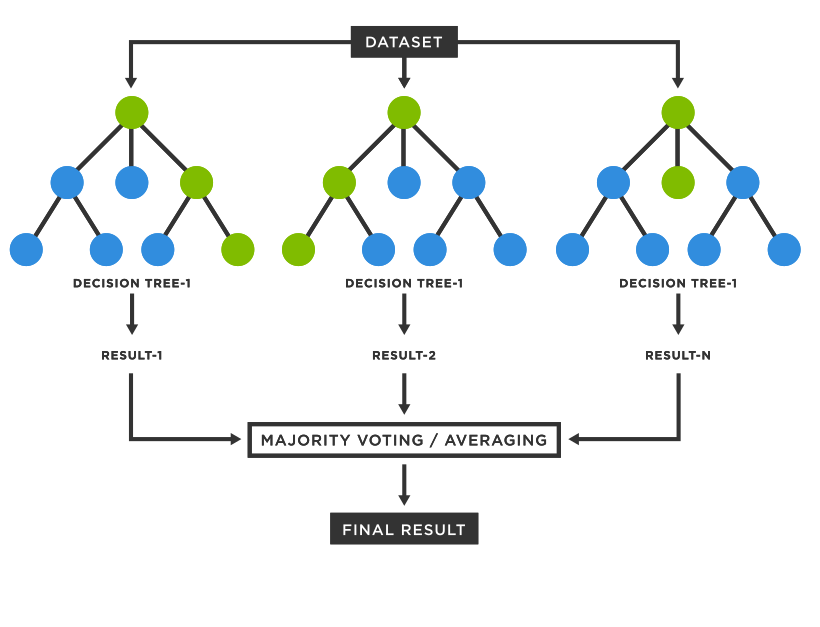
\includegraphics[width=0.7\linewidth]{TemplateTesi//immagini/random-forest-diagram.png}
    \caption{Processo decisionale all'interno del Random Forest \cite{immrf}}
    \label{fig:randomforest}
\end{figure}
\subsection{eXtreme Gradient Boosting}
Extreme Gradient Boosting (XGB)\cite{XGB} è un algoritmo di ML che, come random forest, si basa sul concetto di ensemble, ovvero sfrutta una aggregazione di modelli di conoscenza più deboli per ottenere una predizione più accurata; ogni nuovo albero viene addestrato sugli errori del precedente in un processo detto boosting.

Il termine "gradient boosting" deriva dall'idea di "potenziare" o migliorare un singolo modello "debole" combinandolo con una serie di altri modelli deboli per generare un modello "forte" collettivo. Il gradient boosting è un'estensione del boosting in cui il processo di generazione dei modelli deboli è formalizzato come un algoritmo "gradient descent" su una funzione obiettivo.
Il Gradient Boosting genera risultati mirati per il modello successivo nel tentativo di minimizzare gli errori.
Le loss function utilizzabili con XGB variano in base al contesto di utilizzo, nel caso della classificazione binaria è generalmente utilizzata la "Log Loss", questa quantifica il prezzo pagato per l'imprecisione delle previsioni nei problemi di classificazione. La log loss penalizza gli errori nella classificazione tenendo conto della probabilità di classificazione \cite{xgbloss1,xgbloss2,XGBNvidia}. 

\subsection{Adaptive Boosting }
Adaptive Boosting (ADA) rappresenta un algoritmo di boosting che mira a creare un classificatore forte combinando una serie di classificatori deboli. Questi classificatori deboli, noti come "decision stump" ( alberi decisionali con una sola diramazione), vengono utilizzati come punto di partenza per la costruzione graduale del modello finale. 
Durante il processo, vengono assegnati pesi equi a ogni record classificato e successivamente si attribuiscono pesi più significativi alle classificazioni errate, in modo da creare un nuovo modello debole\cite{ada1}. Questi passaggi vengono ripetuti fino a quando i modelli deboli generati, ognuno con pesi diversi, vengono aggregati in un unico modello forte in grado di eseguire la classificazione in maniera efficace, come visibile in figura \ref{fig:ada}\cite{ada2}.

\begin{figure}[H]
    \centering
    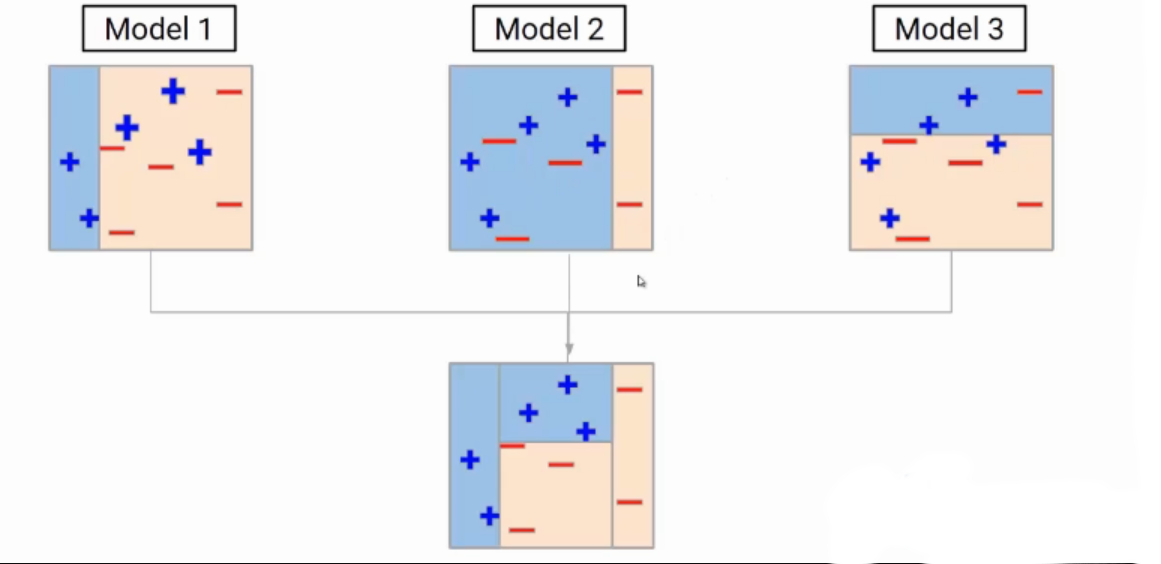
\includegraphics[width=0.75\linewidth]{TemplateTesi//immagini/dsd.jpg}
    \caption{Processo di creazione del modello forte per ADA \cite{ada2}}
    \label{fig:ada}
\end{figure}
\section{Tuning degli iperparametri}
Nel ML, gli iperparametri sono parametri esterni al modello che ne descrivono le caratteristiche. Attraverso il processo di "tuning degli iperparametri", si ricerca la combinazione ottimale di valori per questi parametri al fine di massimizzare le prestazioni del modello. L'obiettivo è trovare i valori migliori per gli iperparametri che permettano di ottenere il miglior modello possibile.

Due tecniche utilizzate per la ricerca degli iperparametri sono:
\begin{itemize}
    \item \textbf{Random Search}:
    un metodo di tuning degli iperparametri che coinvolge la selezione casuale dei valori degli stessi all'interno di un certo intervallo. Durante il processo di Random Search, vengono generate diverse combinazioni casuali di valori degli iperparametri e viene addestrato un modello per ciascuna combinazione. Successivamente, le prestazioni di ogni modello vengono valutate utilizzando una metrica di valutazione appropriata, come l'accuracy. Infine, si seleziona la combinazione di iperparametri che ha fornito le migliori prestazioni
    \item \textbf{Grid Search}:
    La Grid Search prevede la definizione di una griglia di possibili valori per ciascun iperparametro. Per ogni combinazione di valori degli iperparametri nella griglia, viene addestrato un modello e le sue prestazioni vengono valutate utilizzando le metriche di valutazione scelte.

    Il processo di Grid Search esplora in maniera sistematica tutte le possibili combinazioni di valori degli iperparametri specificate nella griglia. Ad esempio, se abbiamo due iperparametri A e B con tre possibili valori per A e due possibili valori per B, la Grid Search esplorerà un totale di sei combinazioni.
\end{itemize}
Spesso tali tecniche sono usate in combinazione con processi di cross validation, spiegati precedentemente
\section{PostProcessing: XAI}
L'opacità e la mancanza di trasparenza dei  modelli di ML possono portare a dubbi sulla loro affidabilità e accettabilità. L'Explainable Artificial Intelligence (XAI) è emersa come una disciplina che mira a risolvere questo problema, cercando di rendere i modelli di ML più comprensibili e interpretabili per gli esseri umani.

L'obiettivo fondamentale della XAI è quello di fornire spiegazioni comprensibili sul perché un modello di ML ha preso una determinata decisione o ha fatto una determinata previsione. Queste spiegazioni possono aiutare gli utenti a comprendere il ragionamento del modello e a identificare potenziali pregiudizi, errori o vulnerabilità nel processo decisionale. La trasparenza e l'interpretabilità dei modelli di IA sono diventate sempre più importanti in diversi contesti, come la medicina, la finanza, la sicurezza e molti altri settori in cui le decisioni basate sull'IA possono avere conseguenze significative sulla vita delle persone \cite{aicambiatutto}.


La XAI comprende due approcci principali: \textbf{model-based} e \textbf{post-hoc}.
L'approccio model-based si concentra sulla costruzione di modelli interpretabili fin dall'inizio. Questi modelli sono progettati per essere esplicitamente interpretabili e trasparenti, consentendo agli utenti di comprendere facilmente le decisioni prese.

D'altra parte, l'approccio post-hoc si concentra sulla spiegazione dei modelli di ML "black box" , che possono essere complessi e difficili da interpretare. L'obiettivo è fornire spiegazioni esterne al modello stesso, senza modificarne la struttura. Questo approccio è particolarmente utile quando si lavora con modelli di ML complessi come le Deep Neural Network (DNN). Alcuni esempi di approcci post-hoc includono LIME (Local Interpretable Model-Agnostic Explanations) e SHAP (SHapley Additive exPlanations), che generano spiegazioni locali per le singole previsioni.

Oltre alla distinzione tra approcci model-based e post-hoc, è possibile classificare i modelli di ML in \textbf{white box} e \textbf{black box}. I modelli white box sono quelli in cui la struttura e il funzionamento sono completamente trasparenti e comprensibili. Esempi di modello white box sono la linear regression, in cui i coefficienti delle variabili di input forniscono informazioni dirette sul loro impatto sul risultato, e il decision tree dove la struttura dell'albero ci fornisce i dettagli sul processo decisionale (come visibile in figura \ref{fig:ibmtrees}). Al contrario, i modelli black box sono caratterizzati da una mancanza di trasparenza e comprensibilità.Le DNN sono un esempio di modello black box, poiché la complessità delle loro connessioni rende difficile comprenderne il funzionamento.

Nel contesto della XAI, sono anche rilevanti i concetti di \emph{agnosticismo} e di \emph{scope}. Le spiegazioni, frutto della XAI, possono essere categorizzate come \textbf{model-agnostic} o \textbf{model-specific} e, dal punto di vista dello scope,  \textbf{global explanation} o \textbf{local explanation}.

Le spiegazioni model-agnostic sono indipendenti dal modello di ML utilizzato e sono applicabili a una vasta gamma di modelli. Queste spiegazioni cercano di estrarre informazioni  rilevanti per la comprensione generale del modello. Ad esempio, SHAP è un approccio model agnostic che calcola l'importanza delle caratteristiche per una specifica previsione.

D'altra parte, le spiegazioni model-specific sono specifiche per un determinato modello di ML. Queste spiegazioni sfruttano le proprietà interne del modello per fornire spiegazioni dettagliate delle decisioni prese. Ad esempio, le attribuzioni dei pesi delle connessioni neurali in una GAN sono spiegazioni specifiche che evidenziano il contributo di ogni connessione alla generazione dei dati.

Le spiegazioni globali sono orientate a fornire una comprensione generale del modello di ML nel suo complesso. Queste spiegazioni esaminano le regole generali e le relazioni tra le variabili di input e output. Le spiegazioni locali, invece, si concentrano su singole istanze o previsioni, offrendo una comprensione dettagliata dei fattori che hanno contribuito a una specifica decisione.


\subsection{LIME}
LIME, abbreviazione di Local Interpretable Model-Agnostic Explanations, è una tecnica appartenente all'Explainable Artificial Intelligence (XAI). Essa si basa sull'utilizzo di "Modelli Locali Surrogati" per spiegare le decisioni prese dal modello di ML in esame. Il funzionamento di LIME si basa sull'addestramento di tali modelli surrogati.

Per comprendere le motivazioni alla base di una specifica previsione, LIME esegue una serie di test sulle previsioni quando vengono variati i valori delle features nei dati del modello generale. A tal fine, LIME genera un nuovo insieme di dati costituito da campioni perturbati e le relative previsioni del modello generale. Successivamente, su questo nuovo insieme di dati, LIME addestra un modello surrogato locale, che viene pesato in base alla vicinanza delle istanze campionate rispetto all'istanza di interesse iniziale. L'obiettivo del modello surrogato ottenuto è quello di essere una buona approssimazione delle previsioni del modello di ML a livello locale, senza necessariamente essere un'ottima approssimazione globale. Questo tipo di precisione è definito anche come fedeltà locale.\cite{interpretableml}

Dal punto di vista matematico il funzionamento del modello surrogato è descritto nella seguente maniera 

$$\text{explanation}(x)=\arg\min_{g\in{}G}L(f,g,\pi_x)+\Omega(g)$$

dove:
\begin{itemize}
   \item x= Dato in input (un record)
    \item f= Modello generale
    \item g= Modello surrogato
    \item G= Famiglia di modelli interpretabili
    \item \(\pi_x\)= misura di prossimita ad x
    \item \(\Omega(g)\)= usato per regolare la complessità del modello surrogato g
    \item \(L(f,g,\pi_x)\)= misurerà l'infedeltà di g nel fare approssimazioni di f nella località $\pi_x$.
\end{itemize}
ottenendo così i seguenti passaggi fondamentali:
\begin{itemize}
    \item Si seleziona l'istanza per la quale si desidera avere una spiegazione della previsione del modello black box.
    \item Si perturba il dataset e si calcolano le previsioni del modello black box per il nuovo dataset pesando i nuovi dati in base alla loro vicinanza con l'istanza scelta.
    \item Si addestra il modello surrogato sul set di dati con le variazioni.
    \item Otteniamo la previsione della istanza iniziale interpretando il modello locale surrogato.
\end{itemize}
\begin{figure}[H]
    \centering
    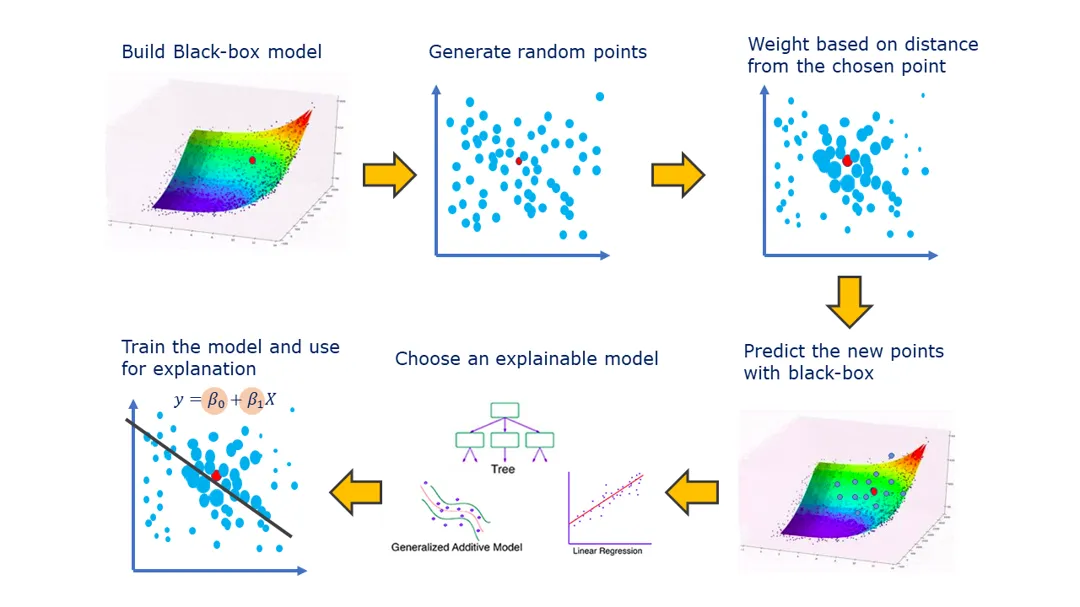
\includegraphics[width=1\linewidth]{TemplateTesi//immagini/limesteps.png}
    \caption{Steps di LIME \cite{immstepslime}}
    \label{fig:enter-label}
\end{figure}
\subsection{SHAP}
SHAP, acronimo di SHapley Additive exPlanations, è una tecnica di XAI che trova le sue radici nella teoria dei giochi. In particolare, si basa sul concetto di Shapley Values.
Nella teoria dei giochi, gli Shapley Values sono una misura del contributo che ciascun giocatore apporta in un gioco cooperativo. Nel contesto della teoria dei giochi, consideriamo una "coalizione" come un gruppo di persone diverse che collaborano durante lo svolgimento di un gioco. Gli Shapley Values ci forniscono una misura di quanto ciascun giocatore abbia contribuito all'interno della coalizione.
In modo più formale, il valore di Shapley del valore \emph{val} di una feature è il suo contributo al risultato finale, ponderato e sommato su tutte le possibili combinazioni di valori delle features. Questo concetto può essere espresso mediante la seguente formula \cite{interpretableml}:
$$\phi_j(val)=\sum_{S\subseteq\{1,\ldots,p\} \backslash \{j\}}\frac{|S|!\left(p-|S|-1\right)!}{p!}\left(val\left(S\cup\{j\}\right)-val(S)\right)$$
dove  $S$ è un sottoinsieme delle features utilizzate nel modello e $p$ il numero di caratteristiche.  

Definito $x$ come il vettore dei valori delle features dell'istanza da spiegare,
\(val_x(S)\) è la previsione per i valori delle features nell'insieme S che sono marginalizzati rispetto alle caratteristiche non incluse nell'insieme S:
$$val_{x}(S)=\int\hat{f}(x_{1},\ldots,x_{p})d\mathbb{P}_{x\notin{}S}-E_X(\hat{f}(X))$$

Il funzionamento di SHAP quindi consiste nel calcolo degli Shapley Values per ogni feature e istanza in input, offrendo in output una spiegazione su come ciascuna feature contribuisce alla previsione del modello.
Come visibile in figura \ref{fig:risultatiSHAP}
per ogni feature presente nel grafo è riportato il valore del proprio shapley value,andando a darci una rappresentazione dell'apporto di ogni feature per la risoluzione del problema in analisi.
In questo caso ci vengono presentati in ordine decrescente di impatto sulla classificazione, mostrandoci come le features "MedInc" e "Latitude" abbiano contribuito in modo positivo nella scelta di una delle due classi del problema, la feature "Longitude", invece, ha contribuito nel senso opposto alle prime due.
\begin{figure}[H]
    \centering
    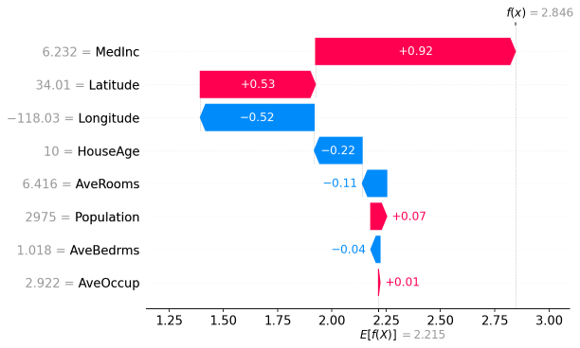
\includegraphics[width=0.75\linewidth]{TemplateTesi//immagini/shapexample.png}
    \caption{Esempio di Visualizzazione risultati di SHAP \cite{ImmShapExample}}
    \label{fig:risultatiSHAP}
\end{figure}


\subsection{Counterfactual Explanations}
Counterfactual Explanations è una tecnica che fornisce una  spiegazione sui risultati di un modello che si basa sulla modifica dei valori delle features di un'istanza in input al fine di comprendere come tali modifiche influenzino le decisioni dello stesso.
In particolar modo una "counterfactual explanation" di una predizione ci \textbf{descrive i cambiamenti più piccoli da effettuare sui valori delle features affinchè la predizione fornita dal modello cambi} (figura \ref{fig:counterfactual}).
Ritengo importante sottolineare l'importanza dell'utilizzo di questa tecnica nel contesto della riabilitazione, poiché non solo è essenziale adottare le tecniche specifiche indicate dai professionisti, ma anche adattare il proprio stile di vita in base agli obiettivi desiderati,le spiegazioni generate possono essere un suggerimento sul percorso da seguire per rientrare nei propri obiettivi.


Il processo di generazione delle conterfactual explanations coinvolge diverse fasi. Inizialmente, viene selezionato un campione per cui si desidera ottenere una spiegazione. Successivamente, vengono applicate modifiche al campione in input per creare un'istanza alternativa. Queste modifiche possono riguardare una o più features, modificandone i valori e potendo selezionare sia le features da modificare che il range della possibile modifica.

Le modifiche effettuate sulle features possono avvenire seguendo meccanismi differenti \cite{interpretableml}:
\begin{itemize}
    \item Variazioni Randomiche: Si perturbano in maniera casuale le features, all'interno degli eventuali range indicati, valutandone poi l'outcome del modello.

    \item Algoritmi Genetici: 
    
    È possibile utilizzare algoritmi genetici come il Nondominated Sorting Genetic Algorithm (NSGA-II), questo prende ispirazione e applica le leggi di Darwin sulla "Survival of the fittest" o "Sopravvivenza del più adatto" dove il più adatto è la counterfactual explanation che minimizza un vettore di funzioni obiettivo $(o_1,o_2,o_3,o_4)$.
    \item Approccio di Wachter:

    
    Consiste nella minimizzazione della seguente "loss function"
    $$L(x,x^\prime,y^\prime,\lambda)=\lambda\cdot(\hat{f}(x^\prime)-y^\prime)^2+d(x,x^\prime)$$
    dove:
    \begin{itemize}
        \item Il primo termine è la distanza al quadrato tra la previsione del modello per il counterfactual x' e il risultato desiderato y'
        \item  Il secondo termine è la distanza d tra l'istanza x da spiegare e il counterfactual x'
        \item d è definita come la distanza di Manhattan pesata con l'inverso della deviazione mediana assoluta di ogni feature (MAD)
        $$d(x,x^\prime)=\sum_{j=1}^p\frac{|x_j-x^\prime_j|}{MAD_j}$$

        \item il parametro \( \lambda \)  serve per il bilanciamento dei contributi del primo e secondo termine all'interno della loss function 
    \end{itemize}
    
\end{itemize}
\begin{figure}[H]
    \centering
    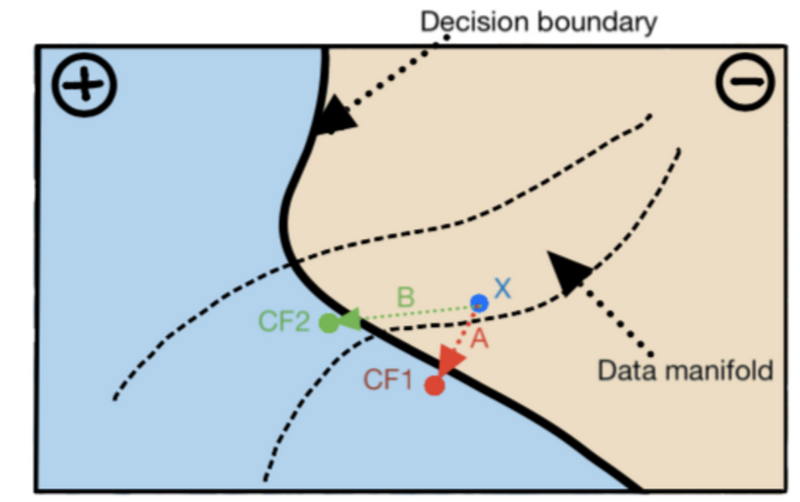
\includegraphics[width=0.7\linewidth]{TemplateTesi//immagini/cf.png}
    \caption{Funzionamento Grafico della Counterfactual Explanations \cite{immcf}}
    \label{fig:counterfactual}
\end{figure}


\section{Explorative Data Analysis (EDA)}
L'EDA svolge un ruolo cruciale nei processi di ML. Prima di poter applicare algoritmi di ML sui dati, è necessario comprendere la loro natura e struttura. 
L'EDA fornisce una panoramica iniziale che aiuta a rispondere a domande chiave come: quali variabili sono rilevanti per il problema in esame? Esistono correlazioni o pattern che possono influire sulla performance del modello? Sono presenti valori mancanti o outliers che richiedono un'attenzione particolare?
È quindi una fase fondamentale per il processo di costruzione di un modello.

Di seguito verranno elencate alcune delle tecniche o valori da tenere in considerazione durante questa fase di esplorazione dei dati.
\subsection{Distribuzione di Probabilità Normale}
In Data Science,il calcolo  della distribuzione normale è uno strumento ampiamente utilizzato per descrivere e analizzare le distribuzioni delle variabili.
La distribuzione normale, anche nota come distribuzione di Gauss, è una distribuzione continua simmetrica che rappresenta molte variabili nel mondo reale. È caratterizzata dalla sua forma a campana ( figura \ref{fig:distrnorm}) e dalla sua funzione di densità di probabilità definita dalla seguente equazione:
$$f(x,\mu, \sigma) = \frac{1}{{\sigma \sqrt{2\pi}}} \cdot e^{-\frac{{(x - \mu)^2}}{{2\sigma^2}}}$$
dove:
\begin{itemize}
    \item $\sigma^2$=varianza
    \item $\mu$=media
\end{itemize}  



\begin{figure}[H]
    \centering
    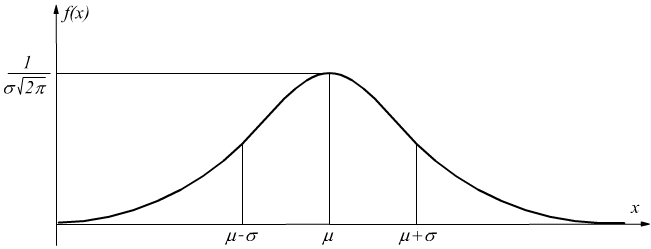
\includegraphics[width=0.5\linewidth]{TemplateTesi//immagini/distribuzionenormale.png}
    \caption{ Forma classica di una Distribuzione Normale \cite{ImmGaussiana}}
    \label{fig:distrnorm}
\end{figure}
\subsection{Coefficiente di Correlazione: HeatMap}
Il coefficiente di correlazione è una misura statistica che indica la relazione tra due variabili. Questo coefficiente varia da -1 a 1, dove un valore di -1 indica una correlazione negativa perfetta, 1 indica una correlazione positiva perfetta e 0 indica una mancanza di correlazione lineare tra le variabili.

Per calcolare il coefficiente di correlazione tra due variabili X e Y, possiamo utilizzare la seguente formula:

$$\rho(X,Y)=\frac{\sigma{_X_Y}}{\sigma_X \sigma_ Y}$$
dove:
\begin{itemize}
    \item $\sigma{_X_Y}$=covarianza tra X e Y
    \item $\sigma_X$=deviazione standard di X
    \item $\sigma_Y$=deviazione standard di Y
\end{itemize}

Uno dei metodi di visualizzazione più comodi per questa fase esplorativa è la visualizzazione tramite HeatMap dei valori dei coefficienti di correlazione tra le features, visibile in figura \ref{fig:heatmapesempio}.
\begin{figure}[H]
    \centering
    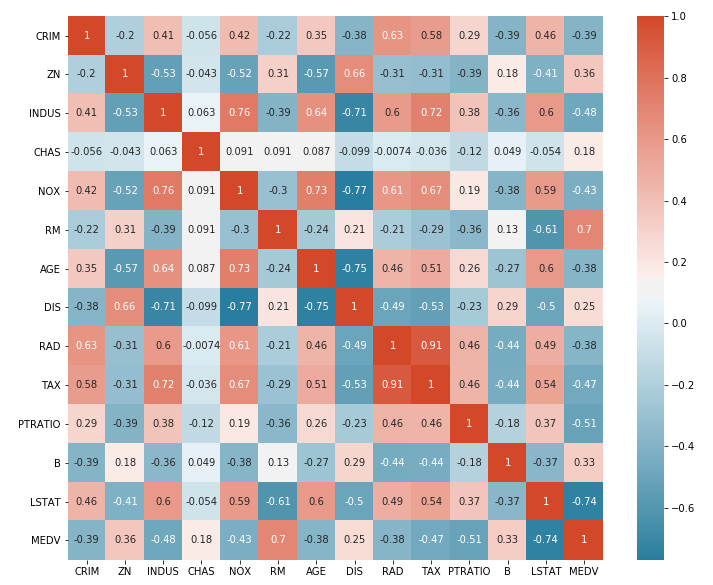
\includegraphics[width=0.5\linewidth]{TemplateTesi//immagini/heatmap esempio.png}
    \caption{Esempio di una Heatmap \cite{ImmHeatMap}}
    \label{fig:heatmapesempio}
\end{figure}
\subsection{MI (Mutual Information) Score}
Tecnica appartenente alla Teoria della Probabilità, calcola la mutua dipendenza di due variabili aleatorie, nel contesto dell'EDA è usata come tecnica di feature selection.
Viene calcolata con la seguente formula:


$$MI(X, Y) = \sum\limits_{y \in Y}\sum\limits_{x \in X} p(x, y) \log \left( \frac{p(x, y)}{p_1(x) \cdot p_2(y)} \right)
$$

dove :
\begin{itemize}
    \item p(x,y):Funzione di distribuzione di probabilità congiunta di X e Y
    \item $p_1(x)$=funzione di distribuzione di probabilità marginale di X
    \item $p_2(y)$=funzione di distribuzione di probabilità marginale di X
\end{itemize}
\end{flushleft}


\clearpage

\clearpage

\chapter{Metodologie di Analisi}
\label{ch:capitolo3}

\begin{flushleft}
    
Nel corso di questo capitolo sarà presentata una panoramica delle metodologie di analisi e delle pipeline (figura \ref{fig:pipeline}) per la costruzione dei modelli, i risultati di tali analisi saranno poi disponibili nel capitolo successivo.
È importante sottolineare che, a causa delle policy aziendali, non sarà possibile fornire il codice scritto.

Segue un elenco delle tecnologie,librerie e degli strumenti utilizzati durante lo stage:
\begin{itemize}
    \item \textbf{Python 3.10}: Tutto il codice da me scritto, dalla creazione dei modelli, alle analisi sui dati è stato in tale linguaggio di programmazione.
    Le librerie utilizzate sono state le seguenti:
    \begin{itemize}
    \item statistics
    \item interpret
    \item dice ml
    \item pandas
    \item numpy
    \item scipy
    \item imblearn
    \item matplotlib
    \item sklearn
    \item seaborn
    \item json
    \item configparser
    \item ydata\_profiling
    \item webbrowser
\end{itemize}
    \item \textbf{Google Colab}: Strumento usato per eseguire i test in parallelo
    \item \textbf{Notion}: Strumento usato per salvare, impostare ed elaborare i risultati dei test
    \item \textbf{Jupiter Notebook}: Strumento usato per creare un ambiente di lavoro più pulito e sequenziale

\end{itemize}

\begin{figure}[H]
    \centering
    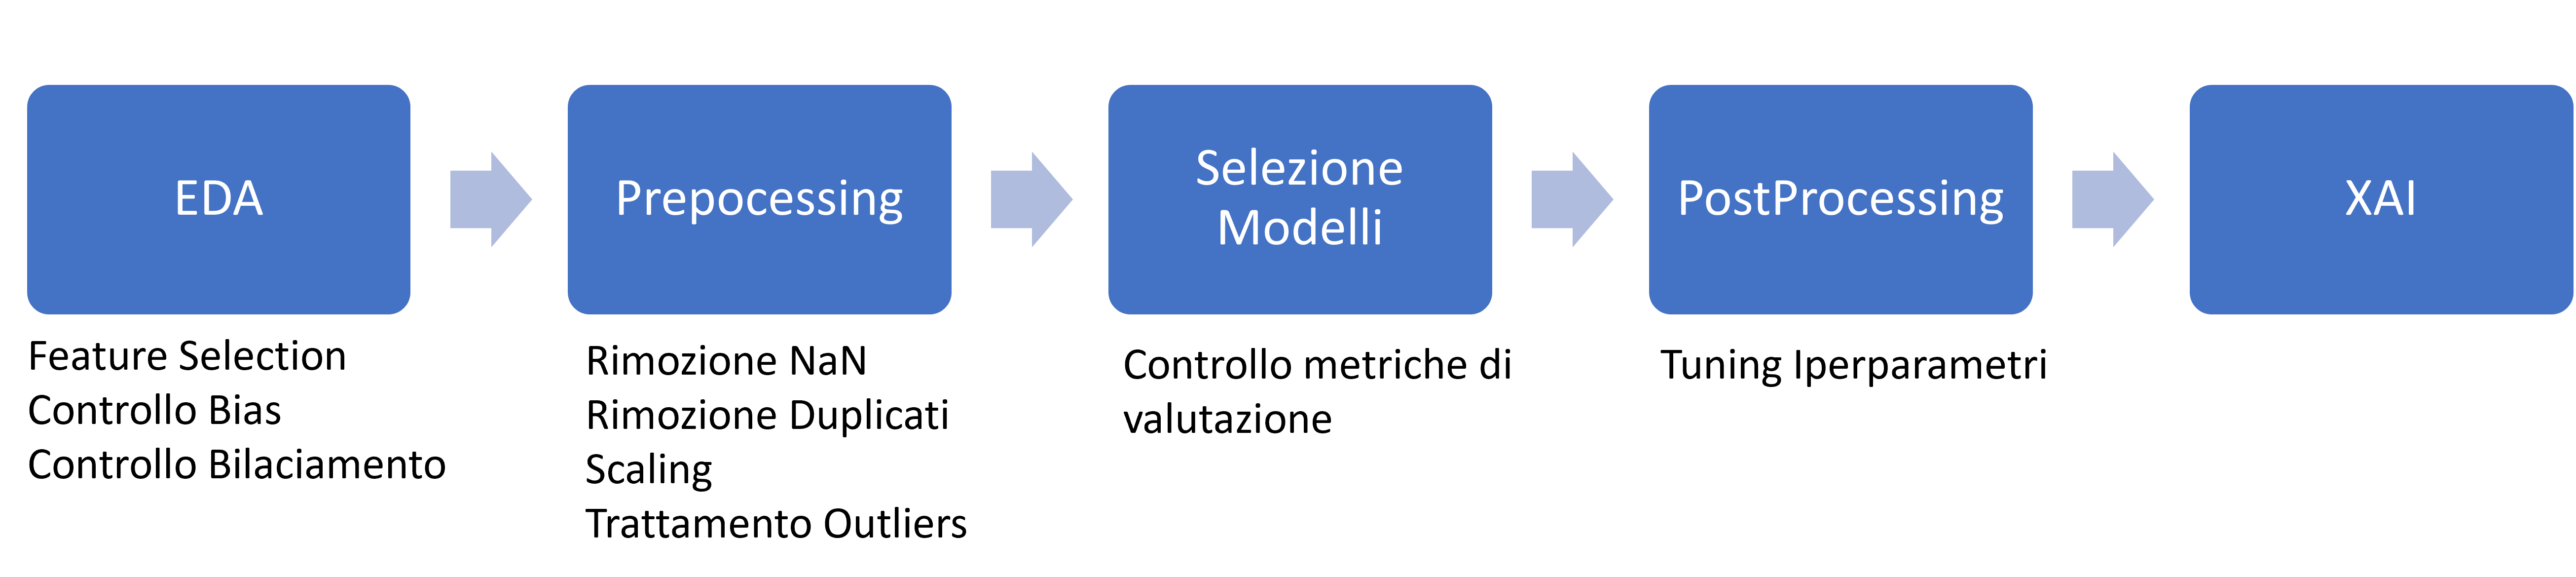
\includegraphics[width=1\linewidth]{TemplateTesi//immagini/pipeline.png}
    \caption{Pipeline di Lavoro Generale attuata}
    \label{fig:pipeline}
\end{figure}

\section{Esplorazione Iniziale dei Dati (EDA)}
L'analisi esplorativa dei dati è un processo fondamentale per comprendere la struttura, le caratteristiche e le relazioni presenti all'interno di un dataset. 
Il primo passo è stato quello di condurre una ricerca per capire le caratteristiche dei i dati clinici relativi alla problematica per la quale si doveva trovare una soluzione. L'obiettivo era identificare i parametri, o feature, più significative per la classificazione del problema precedentemente illustrato.

Durante questa fase, sono stati selezionati i dataset più promettenti dalla piattaforma "Kaggle", effettuando una scrematura che teneva conto della tipologia delle feature presenti, dell'affidabilità delle fonti, della provenienza geografica dei dati e del parametro interno di Kaggle chiamato "Usability". Questo parametro tiene in considerazione le seguenti caratteristiche del dataset: completezza, credibilità e compatibilità.
I dataset analizzati sono strutturati in modo tale che le colonne rappresentino le diverse feature, mentre le righe corrispondono a singoli pazienti, contenendo così i record delle relative feature.
Tali dataset sono visualizzabili in figura~\ref{fig:datasets}.

\begin{figure}[H]
    \centering
    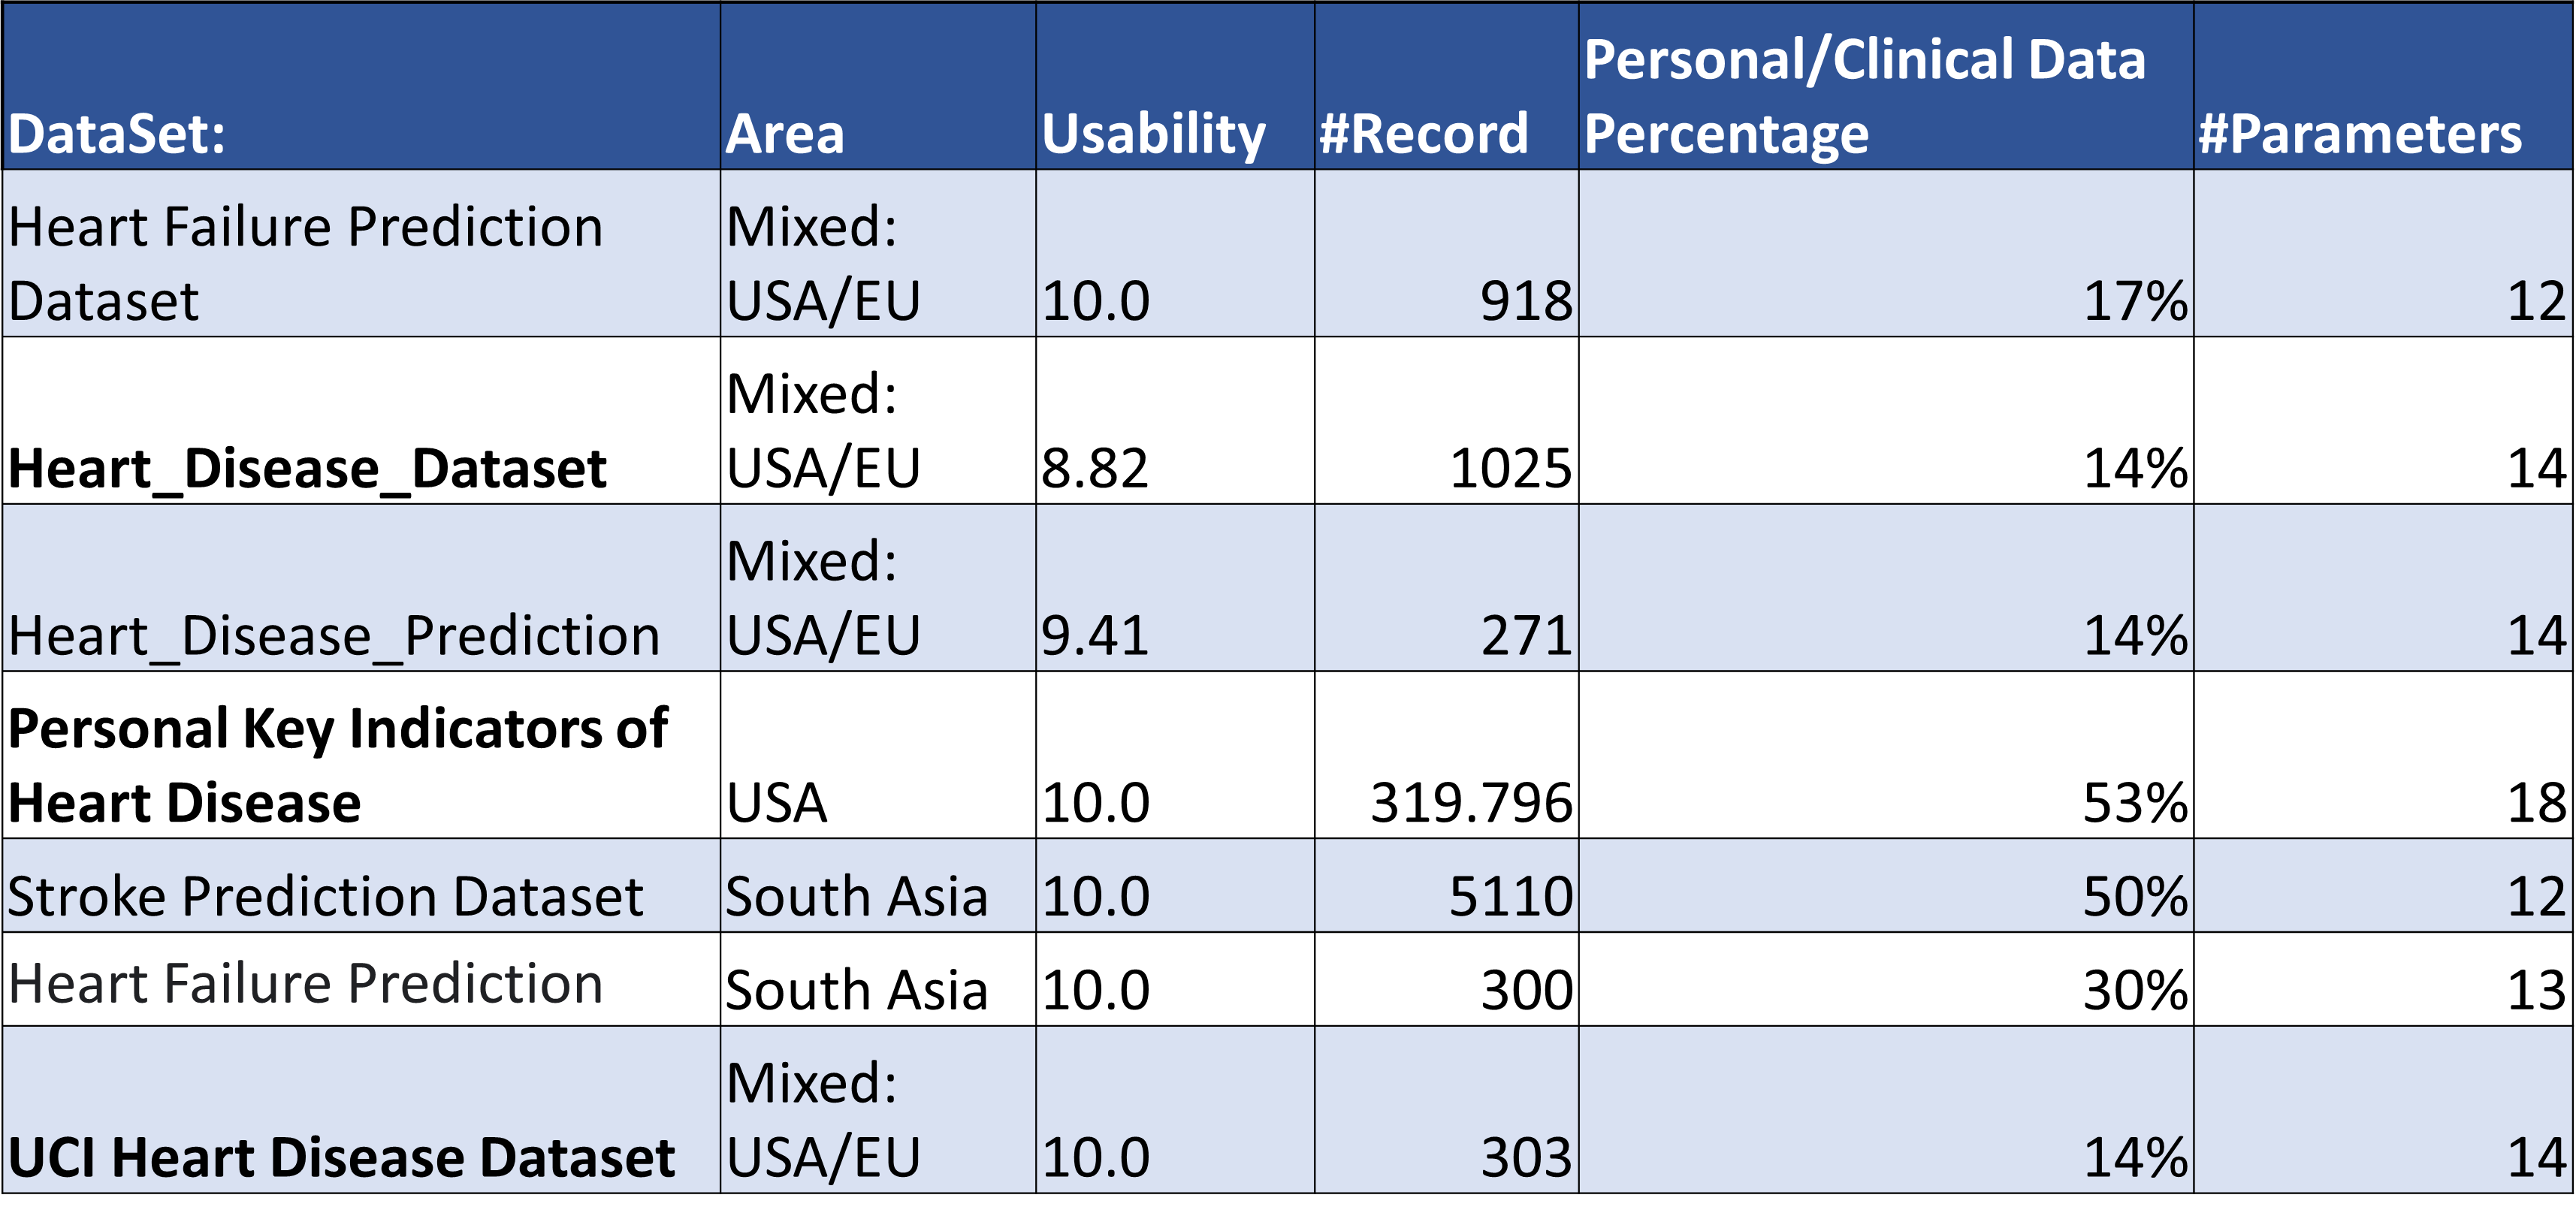
\includegraphics[width=1\linewidth]{TemplateTesi//immagini/datasetsgrassetto.png}
    \caption{I DataSet Selezionati}
    \label{fig:datasets}
\end{figure}

Una volta che i dataset sono stati selezionati, sono state condotte analisi su ciascuno di essi al fine di individuare le feature più significative per la classificazione.
Tra le analisi più importanti effettuate rientrano:
\begin{itemize}
    \item Calcolo dei coefficienti di correlazione tra le feature e tra feature e target
    \item Calcolo delle distribuzioni di probabilità delle feature
    \item Calcolo del MI score 
    \item Analisi qualitativa delle distribuzioni con i clinici
\end{itemize}
Dato il numero considerevole di dataset presi in esame,si riporteranno nella tesi i risultati di tre di essi, che sono coerenti con quelli relativi agli altri dataset: "Heart Disease Dataset (HDD)", "UCI Heart Disease (UCI)" e "Personal Key Indicator of Heart Disease"(PKI).
Su questi tre dataset sono poi state applicate le tecniche di ML studiate.

Il primo e il secondo dataset presentano un'alta percentuale di feature di tipo clinico, mentre il terzo dataset contiene un buon numero di feature che saranno denominati "Personali". Questi dati non derivano da strumentazioni mediche, ma sono accessibili tramite un semplice sondaggio. L'inclusione di questi dati personali è di fondamentale importanza poiché semplifica e velocizza l'acquisizione delle informazioni, evitando di gravare sulle risorse della struttura ospedaliera o richiedere tempo al personale medico.

Prima di presentare le analisi effettuate segue una breve spiegazione delle feature dei dataset menzionati.

\subsubsection{Heart Disease Dataset (HDD)}
%TODO DIRE PROVENIENZA DATI E INTRODURRE LE FEATURES MEGLIO
Il dataset HDD è composto principalmente da features cliniche e i dati provengono dal repository "UCI Machine Learning Repository".
Presenta le seguenti feature:
\begin{itemize}
  \item Age: Età
  \item Sex: Sesso
  \item cp: Tipologia di dolore al petto
  \item trestbps: Pressione Sanguigna a Riposo
  \item chol:colesterolo sierico in mg/d
  \item fbs: glicemia a digiuno
  \item restecg: ECG a riposo
  \item thalach : Massimi Battiti cardiaci raggiunti
  \item exang : angina indotta dall'esercizio fisico
  \item oldpeak:ST depression, ovvero ad un'alterazione del tratto ST dell'elettrocardiogramma di superficie
  \item slope: ST slope
  \item ca: numero di vasi colorati con fluoroscopia
  \end{itemize}

\subsubsection{Personal Key Indicator Of Heart Disease (PKI)}


PKI è un dataset recentemente costruito attraverso l'utilizzo di sondaggi. 
PKI presenta un numero significativamente alto di record, questi sono formati per metà da features di tipo personale.
Seguono le features con le relative domande poste dal sondaggio:


\begin{itemize}
\item HeartDisease: Soggetti che hanno segnalato di aver avuto malattia coronarica o infarto miocardico 
\item BMI: Indice di massa corporea (BMI)
\item Smoking: Hai mai fumato almeno 100 sigarette durante tutta la tua vita? 
\item AlcoholDrinking: Sei un consumatore eccessivo di alcol ? (uomini adulti che assumono più di 14 bevande alcoliche a settimana e donne adulte che assumono più di 7 bevande alcoliche a settimana)
\item Stroke: Ti è mai stato detto che hai avuto un infarto?
\item PhysicalHealth: Pensando alla tua salute fisica, che include malattie e lesioni fisiche, per quanti giorni nei 30 passati la tua salute fisica non è stata buona? 
\item MentalHealth: Pensando alla tua salute mentale, per quanti giorni nei 30 passati la tua salute mentale non è stata buona? 
\item DiffWalking: Hai seri problemi a camminare o salire le scale?
\item Sex: Sei maschio o femmina?
\item AgeCategory: Categoria di età su quattordici livelli
\item Etnia: A che etnia appartieni ?
\item Diabetic : Ti è mai stato detto che hai il diabete?
\item PhysicalActivity: Adulti che hanno dichiarato di fare attività fisica o esercizio durante gli ultimi 30 giorni, al di fuori del lavoro abituale
\item GenHealth: Come descriveresti in generale la tua salute ?
\item SleepTime: In media, quante ore di sonno dormi in un periodo di 24 ore?
\item Asthma: Ti è mai stato detto che hai l'asma?
\item KidneyDisease: Escludendo calcoli renali, infezioni alla vescica o incontinenza, ti è mai stato detto che hai una malattia renale?
\item SkinCancer:Ti è mai stato detto che hai avuto il cancro della pelle?
\end{itemize}

\subsubsection{UCI Heart Disease Dataset (UCI)}


Durante la fase finale del mio stage ho effettuato un'analisi del seguente dataset aggiungendolo al set di dataset esistenti. La decisione di includere questo dataset è stata motivata dalla mia volontà di creare un modello che fosse il più indipendente possibile da complessità aggiuntive. Pertanto, ho cercato di limitare l'applicazione di tecniche sullo stesso, escludendo tecniche di outlier detection e feature selection.

Il dataset in questione è una versione rielaborata del dataset originale noto come "UCI Heart Disease", da cui HDD e gli altri dataset clinici prendono forma. UCI si basa su dati provenienti da quattro database situati in Ungheria, Svizzera, Cleaveland e Long Beach.
Il dataset HDD, a differenza di quest'ultimo, presenta un numero di record superiore rispetto al dataset originale.

Le feature del suddetto dataset e le considerazioni sulle caratteristiche di queste ultime sono identiche a quelle presenti in HDD, quindi non verranno nuovamente menzionate.



\section{Preprocessing dei dati}

In questa sezione,sono illustrate le tecniche di preprocessing che \textbf{sono state applicate ad ogni dataset preso in esame}.
Come spiegato nel capitolo 2, il preprocessing dei dati è una fase cruciale nella preparazione di un dataset per l'applicazione degli algoritmi di ML.
Le tecniche di preprocessing che sono state adottate includono la conversione dei valori nominali in valori numerici, l'eliminazione delle righe con dati mancanti o NaN, l'eliminazione dei duplicati e la normalizzazione dei dati.

\subsection{Conversione dei valori nominali in valori numerici} 
Nei dataset originali, alcune variabili contenevano valori nominali. Per poter utilizzare queste variabili nell'analisi, è stato necessario convertire i valori nominali in valori numerici. Questa conversione è stata effettuata assegnando un valore numerico univoco a ciascuna categoria presente nella variabile nominale. Ad esempio, nel dataset 'PKI' alla variabile 'Sex'i cui valori precedenti erano "Male" e "Female" sono stati assegnati rispettivamente "1" e "0"

\subsection{Eliminazione delle righe con dati mancanti o NaN}
Durante l'analisi dei dataset, è stata rilevata a volte la presenza di alcune righe con dati mancanti o NaN. Sebbene il numero di valori mancanti era relativamente basso si è deciso di eliminare interamente le righe che presentavano dati mancanti o NaN, poiché tale eliminazione non avrebbe compromesso significativamente la rappresentatività dei dati.

\subsection{Eliminazione dei duplicati}
Al fine di evitare la duplicazione dei dati, è stata eseguita un'operazione di rimozione dei duplicati. I duplicati sono stati individuati confrontando l'intera riga di ciascun record con le altre righe del dataset attraverso l'utilizzo di funzioni di libreria.
Se due righe presentavano gli stessi valori in tutte le colonne, tranne l'identificatore univoco del record, una delle righe duplicate è stata eliminata.

\subsection{Normalizzazione dei dati}
La normalizzazione dei dati è una pratica comune nel preprocessing dei dati, che mira a rendere le diverse variabili comparabili nello stesso intervallo di valori. Durante l'analisi, sono state esplorate diverse tecniche di normalizzazione, tra cui MinMax Scaling, Standard Scaler e Robust Scaling. Tutte e tre le tecniche hanno prodotto risultati comparabili, ma alla luce della loro semplicità e della facilità di interpretazione dei risultati, è stata scelta la tecnica di Standard Scaling per la normalizzazione dei dati.

\subsection{Eliminazione degli outlier}
Come specificato nel Capitolo 2, la presenza di outlier può influenzare negativamente i risultati dell'analisi e alterare le conclusioni ottenute. 
Pertanto, è importante identificare e trattare gli outlier in modo appropriato.
Per fare ciò è stata applicata la tecnica di identificazione degli outlier dello Z-score (Figura \ref{fig:zscore}) con valore soglia variabile (generalmente  intorno a 3.5).
Una volta identificati gli outlier è stata rimossa la riga dal dataset che lo rappresentava.

\section{Scelta dei Modelli e Iperparametri}
 Una volta completate le fasi di analisi esplorativa dei dati e preprocessing, si è passato alla fase di addestramento dei modelli.

La scelta del modello è una decisione fondamentale per la creazione di un tool di AI, poiché diversi algoritmi di ML possono adattarsi in modo ottimale a diverse tipologie di dati e problemi specifici. Pertanto, ho valutato  quattro modelli di ML diversi.

\begin{itemize}
    \item SVM
    \item XGB
    \item RF
    \item ADA
\end{itemize}

Durante il processo di selezione del modello, ho considerato diverse metriche di valutazione, tra cui l'accuracy, la precision, la recall, al fine di identificare il modello che avesse le migliori prestazioni nel contesto del mio problema di classificazione.

Dopo aver selezionato il modello, ho valutato le metriche ottenute tramite la cross-validation, utilizzando il 70\% dei dati per l'addestramento e il restante 30\% per i test. Successivamente, ho proceduto con la selezione degli iperparametri.



\subsection{Bilanciamento dei Dataset}

Uno sbilanciamento dei dati, come discusso nel capitolo precedente, può influire negativamente sulle prestazioni del modello, in quanto può verificarsi una predizione sbilanciata o una maggiore sensibilità verso la classe dominante.

Considerando le caratteristiche dei dataset su cui ho lavorato ho valutato l'applicazione delle tecniche di bilanciamento denotate in precedenza, ovvero quelle di undersampling e oversampling.

\subsection{Selezione dei Modelli} 

Dopo aver valutato i quattro modelli di ML, è stata effettuata una comparazione dei  risultati della cross validation. Sulla base delle metriche di valutazione e delle esigenze specifiche del nostro problema (SVM ad esempio è stato scartato poichè i tempi di addestramento erano eccessivamente lunghi, a volte superiori alle 24H per PKI), sono stati selezionati i due modelli che hanno mostrato le migliori prestazioni complessive:  il Modello XGB e il Modello RF .

Tra i due modelli selezionati è stato condotto un ulteriore confronto per determinare il modello più performante. Dopo un'analisi dei risultati, è stato decretato che il Modello RF era il modello più efficace e adatto alle mie esigenze.


\subsection{Ricerca degli iperparametri}
Una volta trovato il modello più performante,l'ultimo passo per migliorare lo score delle metriche è stata la ricerca degli iperparametri, per fare ciò ho adottato un approccio ibrido che combina la random search e la grid search.

Per iniziare, ho utilizzato la random search come tecnica per l'analisi iniziale degli iperparametri. La random search ha consentito l'esplorazione di un'ampia gamma di combinazioni di iperparametri selezionati in maniera casuale. Questo mi ha permesso di ottenere una visione generale delle prestazioni dei modelli con diverse configurazioni di iperparametri, consentendomi di individuare alcune combinazioni più promettenti.

Una volta identificate le combinazioni più promettenti grazie alla random search, ho approfondito la ricerca in un intorno di quegli iperparametri utilizzando la grid search. 

Come spiegato precedentemente la grid search è una tecnica di ricerca esaustiva che valuta tutte le possibili combinazioni di iperparametri specificate in un insieme predefinito, sotto forma di griglia.

Una volta creata la griglia di valori, la grid search ha quindi valutato tutte le possibili combinazioni di questi valori per trovare il set di iperparametri ottimale.

L'approccio ibrido ha dimostrato di essere un metodo efficace per trovare iperparametri ottimali in modo estremamente efficiente. 
Ha permesso di bilanciare la copertura di un'ampia gamma di combinazioni con una ricerca più dettagliata nell'intorno di quelle combinazioni più promettenti.

\section{XAI}
Una volta completata la fase di costruzione dei modelli,
ho messo in pratica tecniche di XAI per fornire spiegazioni dei risultati ottenuti dai miei modelli. In particolare, ho utilizzato sia il metodo LIME che le Counterfactual Explanations, che mi hanno permesso di analizzare il mio problema e le soluzioni sviluppate da un'altra prospettiva. Questo approccio ha arricchito la comprensione dei modelli e ha fornito una maggiore trasparenza riguardo alle ragioni alla base delle previsioni effettuate,di fondamentale importanza nell'ambito clinico.

\subsection{LIME}
L'interpretabilità dei modelli riveste un ruolo fondamentale in ambito clinico, la spiegazione fornita da LIME mi ha aiutato a a identificare le caratteristiche più rilevanti per una determinata predizione e fornire indicazioni su quali aspetti esplorare ulteriormente per confermare la diagnosi.
La collaborazione con esperti medici sarebbe cruciale per una valutazione accurata dei risultati, in quanto l'occhio medico può apportare una conoscenza specialistica e una comprensione approfondita del contesto clinico, fornendo ulteriori interpretazioni e contribuendo alla validazione delle spiegazioni ottenute con LIME.

\subsection{XAI come metodologia di previsione del futuro: creazione di scenari "What If"}

All'interno del contesto dei modelli predittivi che ho generato, ci si concentra principalmente sul "presente", i.e. fare una diagnosi in un paziente in base alle sue variabili clinici in un dato momento. Tuttavia, per estendere le previsioni anche al futuro, ho considerato l'utilizzo delle "Counterfactual Explanations". Queste descrivono le minime variazioni da apportare ai dati affinché si verifichi un cambio di classe.

Mantenendo costante la feature "Age" (con incrementi di 5 anni) all'interno dei miei dati e facendo variare le altre caratteristiche all'interno di range prestabiliti percentuali ho generato degli "What if" scenario per la  valutazione delle future condizioni di salute dei pazienti.
All'interno del contesto della riabilitazione di un paziente, questa osservazione risulta particolarmente significativa per valutare il proprio stile di vita e il suo impatto sul potenziale rischio di mantenere o sviluppare una malattia cardiaca.

Tale utilizzo di questa tecnica mi consente di rispondere alle seguenti domande:
\begin{itemize}
    \item Se mantengo invariato il mio stile di vita, come cambierà nel corso degli anni la probabilità che sviluppi una malattia cardiaca ?
    \item Quali cambiamenti (minimi) devo apportare alla mia vita affinché il rischio di incorrere in una malattia cardiovascolare sia ridotto o eliminato?
\end{itemize}

\end{flushleft}




\clearpage

\clearpage

\chapter{Risultati}
\label{ch:capitolo4}

% --- Inizio del Capitolo 4 ---
Nel corso di questo capitolo, saranno presentati i risultati delle  analisi esplorative, descrivendo le principali scoperte e considerazioni emerse. Inoltre, sarà fornita una valutazione delle tecniche di preprocessing impiegate, evidenziando il loro impatto sulla qualità dei dati. Infine, saranno riportate le metriche dei modelli di ML costruiti, offrendo una visione  delle loro performance rispetto al problema di ricerca iniziale.
Dove possibile saranno riportati i risultati per tutti e 3 i dataset presi in esame, è bene però introdurre il fatto che in alcuni casi non sarà possibile riportare i risultati nella loro interezza poiché le risorse hardware disponibili non sono state in grado di sopportare la potenza di calcolo richiesta dall'impiego di alcune tecniche. 


\section{Risultati EDA}
Si presentano in questa sezione alcuni dei risultati più significativi ottenuti durante la fase esplorativa dei dataset.
Poiché, appunto, il numero di grafici prodotto è molto alto verrà riportata soltanto una selezione.

\subsection{Caratteristiche dei Dataset}
\subsubsection{HDD}


\begin{figure}[H]
    \centering
    \includegraphics[width=0.75\linewidth]{TemplateTesi//immagini/istoHDDtarget.png}
    \caption{Istogramma Relativo alla Feature 'Heart\_Disease' in HDD}
    \label{fig:istoHDDtarget}
\end{figure}
\begin{figure}[H]
    \centering
    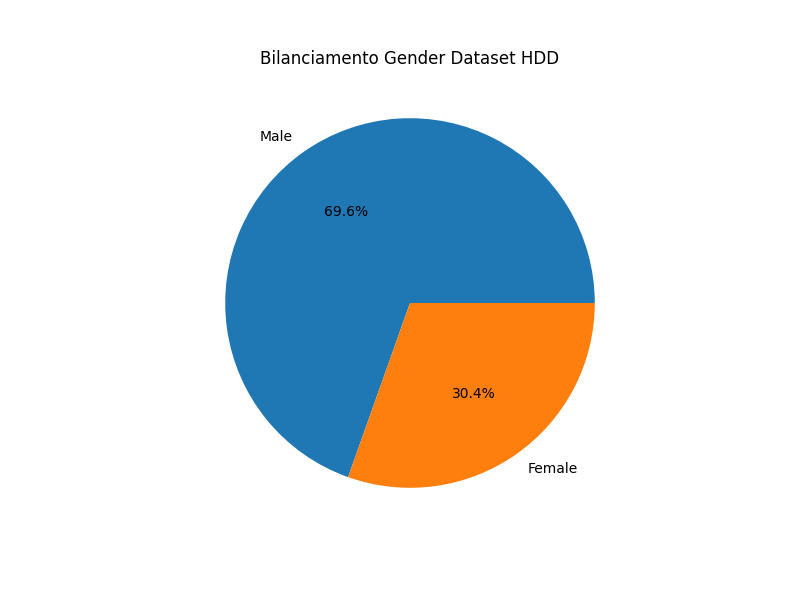
\includegraphics[width=0.75\linewidth]{TemplateTesi//immagini/tortaHDDsex.png}
    \caption{Grafico a Torta Relativo alla Feature 'Sex' in HDD}
    \label{fig:tortaHDDsex}
\end{figure}

\begin{flushleft}
    
Heart Disease Dataset (HDD) si presenta come un dataset abbastanza bilanciato, in quanto il numero di istanze rappresentanti i diversi valori della feature target  ($Heart\_Disease$) sono molto simili tra loro ( come visibile in figura \ref{fig:istoHDDtarget}).

La figura \ref{fig:tortaHDDsex} ci indica  la presenza di un bias nei dati, il numero di pazienti appartenenti al genere femminile è significativamente inferiore a quello di sesso maschile.
Nonostante ciò HDD è il dataset,tra quelli  clinici ,che presenta il maggiore numero di record (figura \ref{fig:datasets}).

\subsubsection{UCI}

\begin{figure}[H]
    \centering
    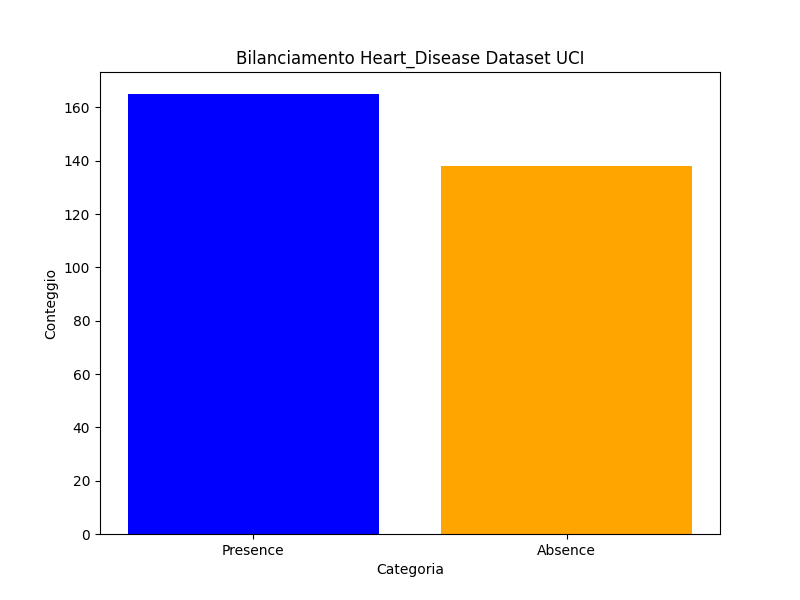
\includegraphics[width=0.75\linewidth]{TemplateTesi//immagini/istoUCItarget.png}
    \caption{Istogramma Relativo alla feature 'Heart\_Disease' in UCI}
    \label{fig:istoUCItarget}
\end{figure}
\begin{figure}[H]
    \centering
    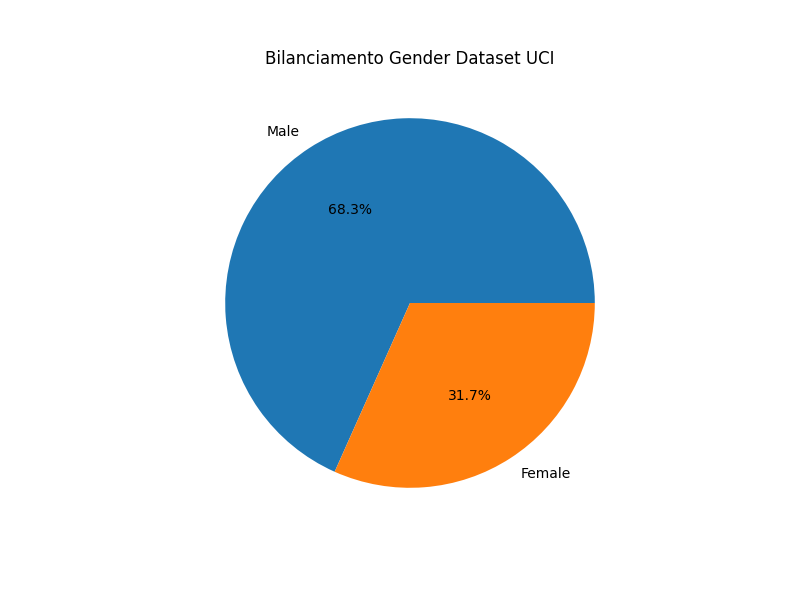
\includegraphics[width=0.75\linewidth]{TemplateTesi//immagini/tortaUCIsex.png}
    \caption{Grafico a Torta Relativo alla feature 'Sex' in UCI}
    \label{fig:tortaUCIsex}
\end{figure}
Come HDD il dataset UCI presenta un buon bilanciamento della feature target ma uno sbilanciamento nella rappresentazione del genere.

\subsubsection{PKI}


  \begin{figure}[H]
    \centering
    \includegraphics[width=0.75\linewidth]{TemplateTesi//immagini/istoPKItarget.png}
    \caption{Istogramma Relativo alla Feature 'Heart\_Disease' in PKI}
    \label{fig:istoPKItarget}
\end{figure}

\begin{figure}[H]
    \centering
    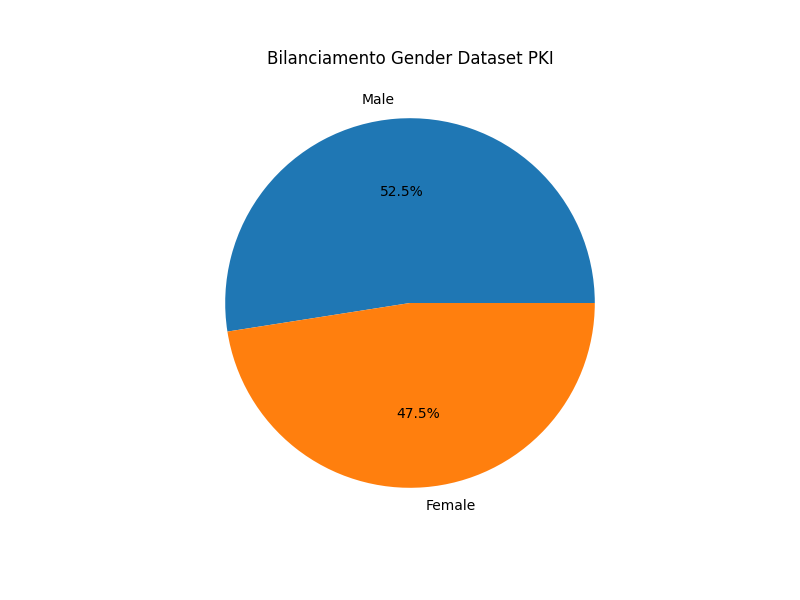
\includegraphics[width=0.75\linewidth]{TemplateTesi//immagini/tortaPKIsex.png}
    \caption{Grafico a Torta Relativo alla Feature 'Sex' in PKI}
    \label{fig:tortaPKIsex}
\end{figure}
Sebbene non presenti bias nella rappresentazione dei sessi all'interno dei dati (visibile in figura \ref{fig:istoPKItarget}) PKI possiede un forte sbilanciamento dei valori della feature "Heart\_Disease" (Questa problematica verrà successivamente trattata). 
È stato importante notare durante la fase esplorativa quali fossero i comportamenti dei valori delle features 'Personali' di PKI e se ci fossero alcune di queste particolarmente sbilanciate.
Tra queste ritengo importante segnalare la feature 'Etnia' (figura \ref{fig:EtniaPKI}), dove osserviamo uno sbilanciamento significativo della presenza di pazienti di etnia caucasica rispetto alle altre.
\begin{figure}[H]
    \centering
    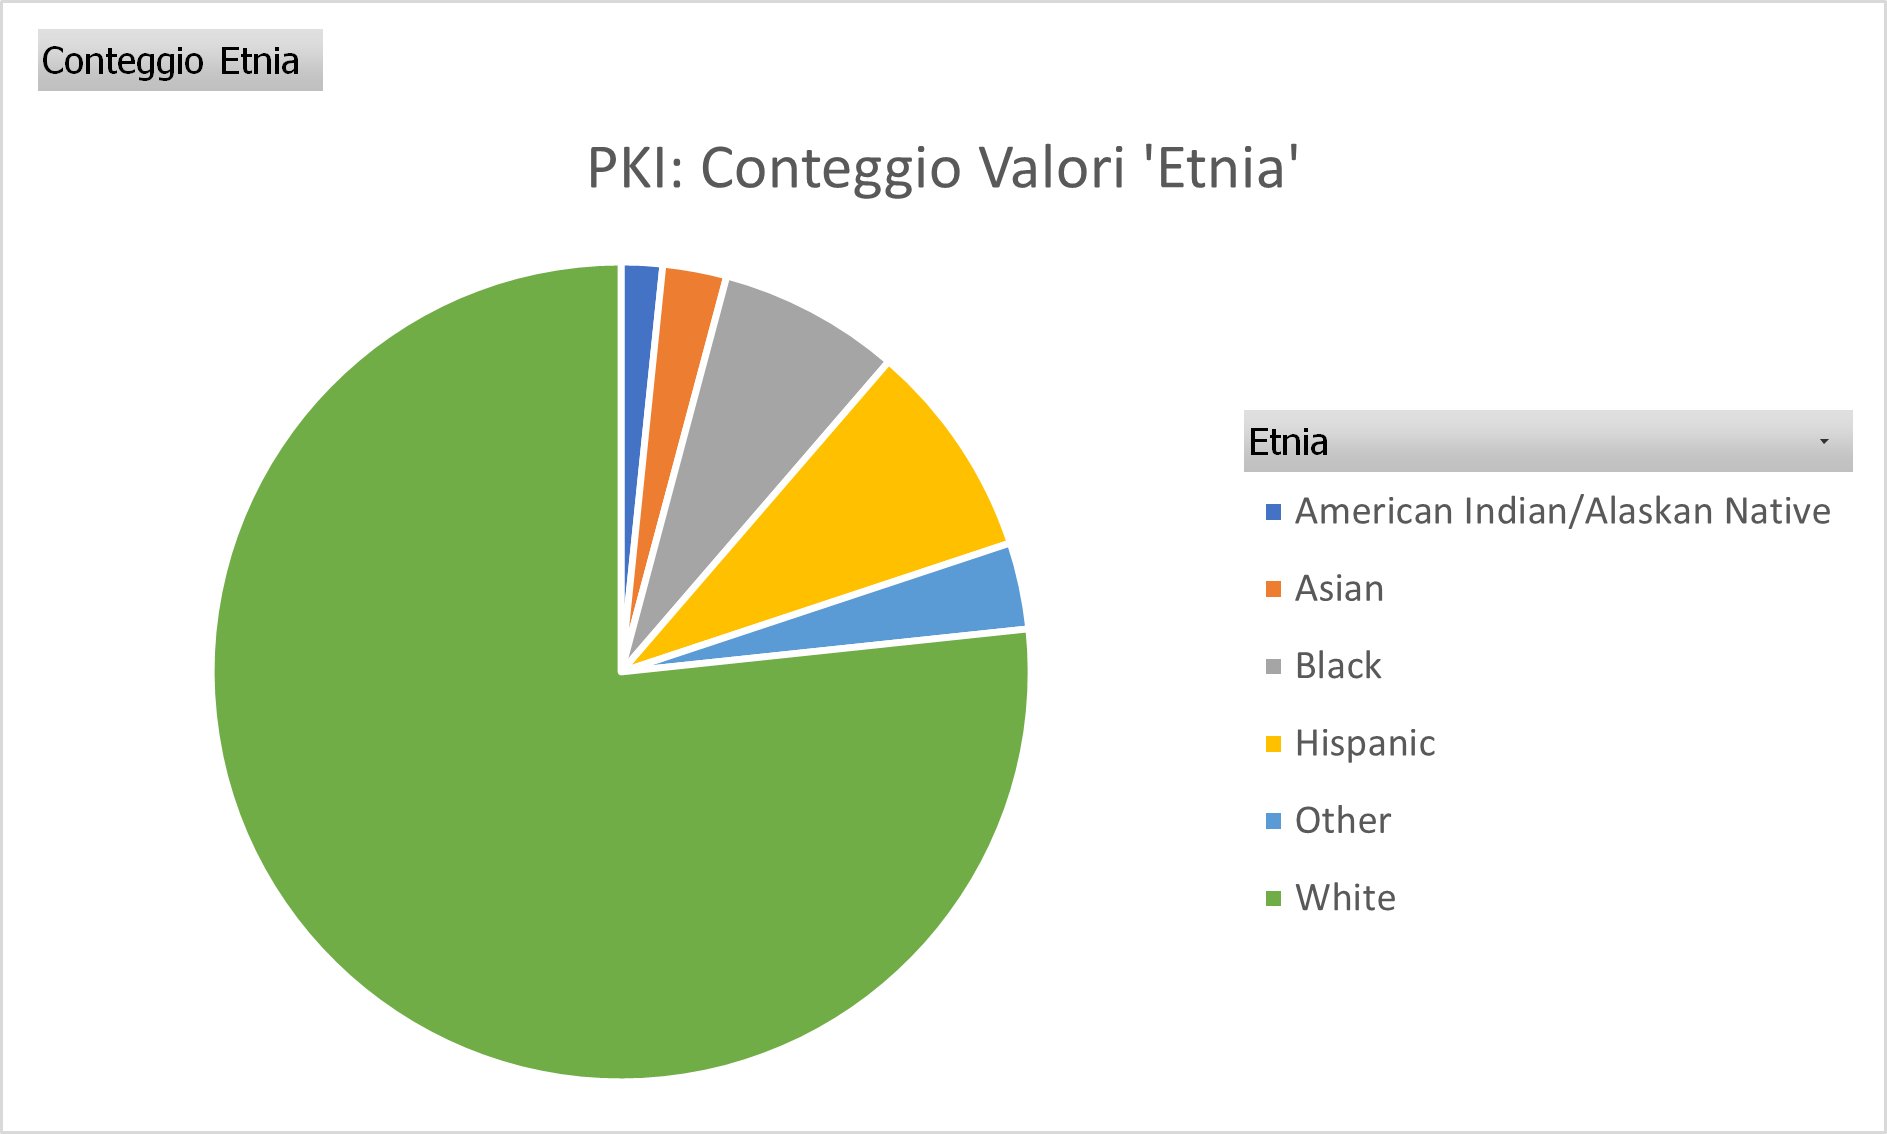
\includegraphics[width=0.75\linewidth]{TemplateTesi//immagini/EtniaRapp.png}
    \caption{Valori della feature categorica che descrive l'etnia di appartenenza dei partecipanti al sondaggio per la costruzione di PKI}
    \label{fig:EtniaPKI}
\end{figure}
\end{flushleft}

\begin{flushleft}
    
Durante la raccolta dei dati è importante cercare di bilanciare la rappresentazione sia dei sessi che dell'etnia.
Un Dataset completo e bilanciato aiuta sensibilmente a garantire la qualità dei risultati generati.
\end{flushleft}

\subsection{Distribuzioni delle feature nei Dataset \label{distribuzionisub}}

Vengono mostrate le distribuzioni di probabilità per i pazienti che presentavano o meno malattie cardiache, rappresentati nel dataset con il valore della feature "Heart\_Disease" rispettivamente 0 e 1. In particolare, sono state selezionate le distribuzioni relative alle feature individuate come le più promettenti. Le distribuzioni presentate nelle figure sottostanti sono state scelte per il loro elevato potenziale discriminatorio, valutato insieme al personale clinico usando un confronto \emph{qualitativo} delle distribuzioni in presenza o assenza di CVD nei pazienti.  
Tutto ciò è fondamentale durante l'allenamento del modello e per ottenere una previsione più accurata.

Nei seguenti grafici, sull'asse x sono riportati i valori delle specifiche feature, che possono essere sia categoriche che continue. Sull'asse y, invece, sono riportati i valori delle distribuzioni, sia per i casi di assenza che presenza di CVD, per facilitarne la comparazione.
\newline
\textbf{Distribuzioni HDD}
\newline



\begin{figure}[H]
    \centering
    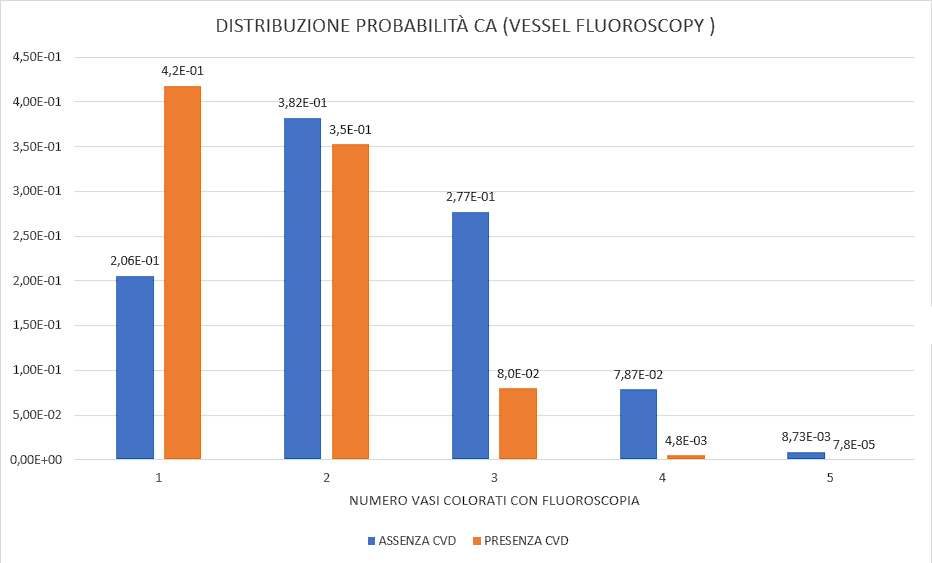
\includegraphics[width=1\linewidth]{TemplateTesi//immagini/CA.png}
    \caption{Distribuzioni di probabilità Fluoroscopia}
    \label{fig:dpHDDfluoro}
\end{figure}

\begin{figure}[H]
    \centering
    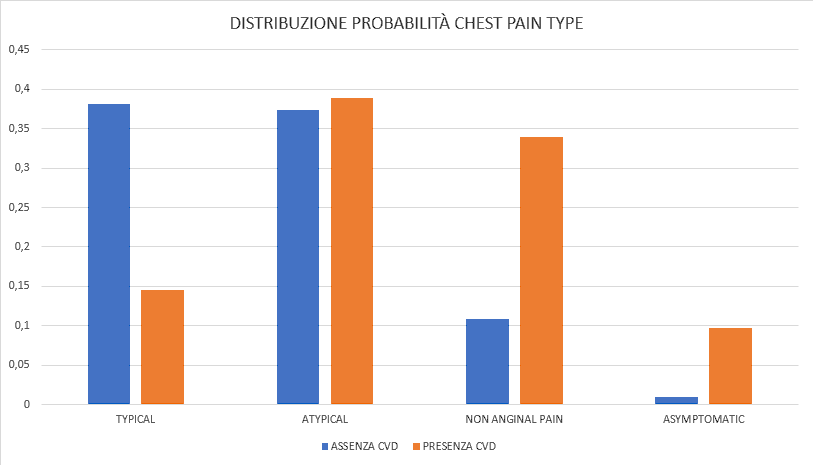
\includegraphics[width=1\linewidth]{TemplateTesi//immagini/CHEPAIN.png}
    \caption{Distribuzioni di probabilità Chest Pain Type}
    \label{fig:dpHDDchepain}
\end{figure}

\begin{figure}[H]
    \centering
    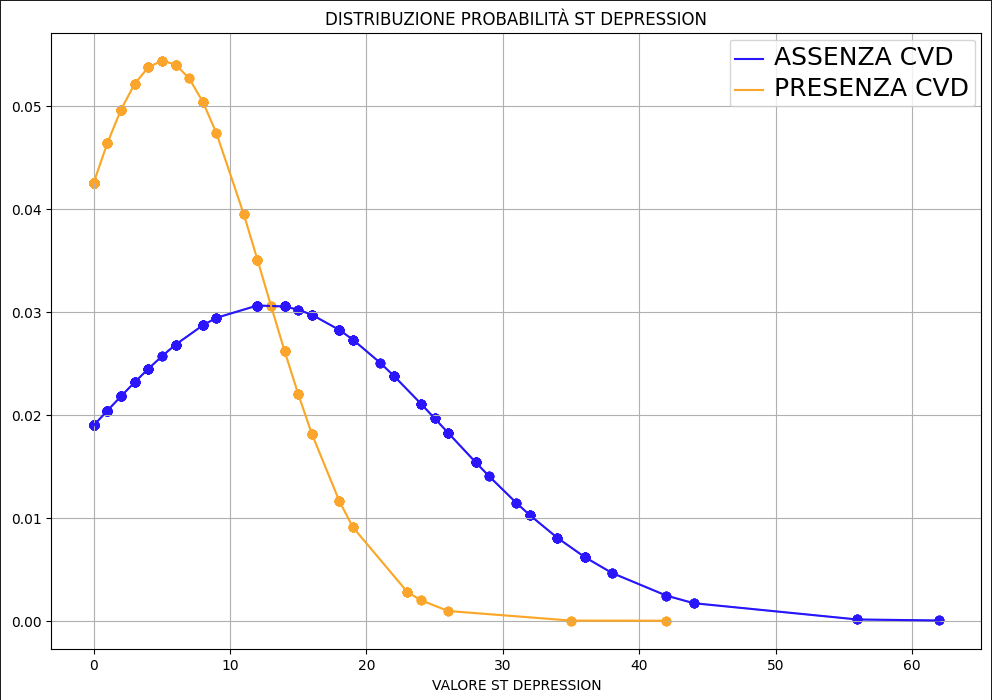
\includegraphics[width=1\linewidth]{TemplateTesi//immagini/stdepre.png}
    \caption{Distribuzioni di probabilità ST depression}
    \label{fig:dpHDDstdepre}
\end{figure}

\begin{figure}[H]
    \centering
    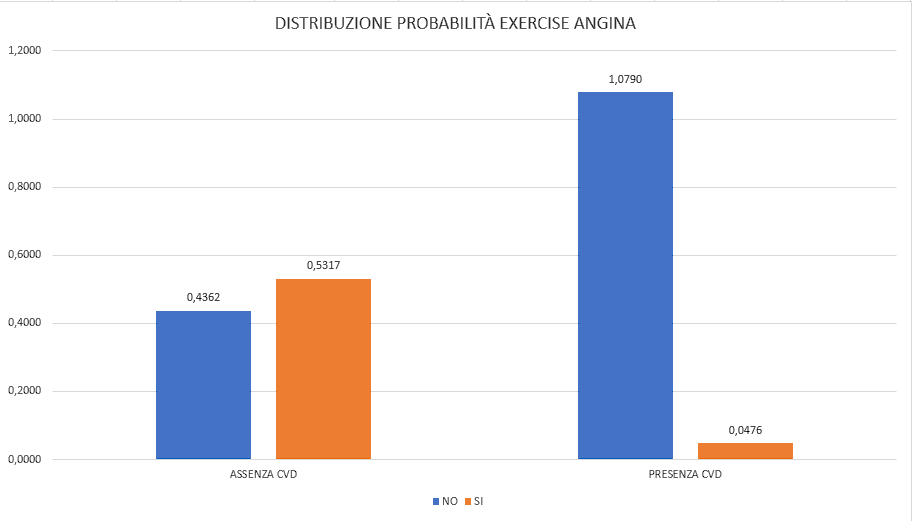
\includegraphics[width=1\linewidth]{TemplateTesi//immagini/EXECANGINA.png}
    \caption{Distribuzioni di probabilità Exercise Angina}
    \label{fig:dpHDDanginaexe}
\end{figure}



\begin{figure}[H]
    \centering
    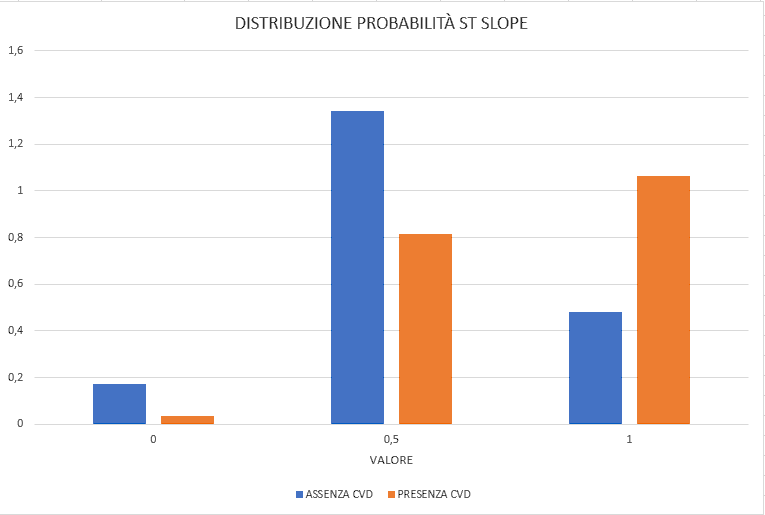
\includegraphics[width=1\linewidth]{TemplateTesi//immagini/SLOPE.png}
    \caption{Distribuzioni di probabilità ST Slope}
    \label{fig:dpHDDSlope}
\end{figure}
\newline
\textbf{Distribuzioni Personal Key Indicator of Heart Disease}
\newline

\begin{figure}[H]
    \centering
    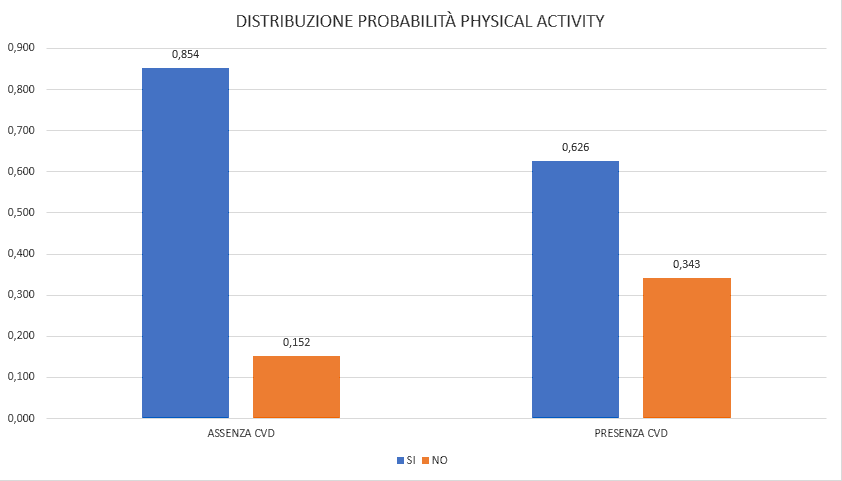
\includegraphics[width=1\linewidth]{TemplateTesi//immagini/PHYACTIVITY.png}
    \caption{Distribuzioni di Probabilità Physical Activity}
    \label{fig:dpPKIphyact}
\end{figure}


\begin{figure}[H]
    \centering
    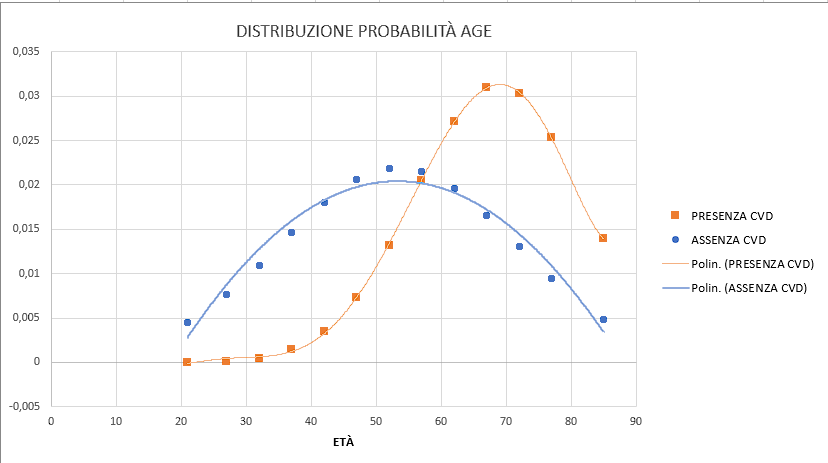
\includegraphics[width=1\linewidth]{TemplateTesi//immagini/AGE.png}
    \caption{Distribuzioni di Probabilità Age}
    \label{fig:dpPKIAge}
\end{figure}
\begin{figure}[H]
    \centering
    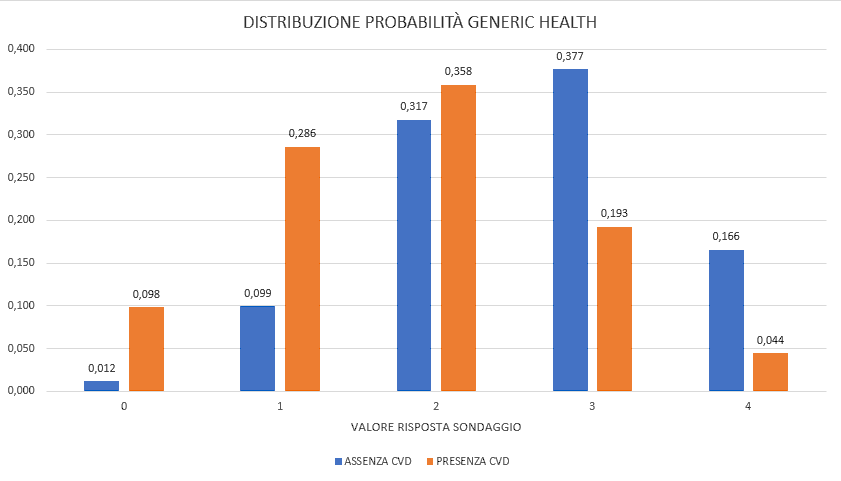
\includegraphics[width=1\linewidth]{TemplateTesi//immagini/GENHEALTH.png}
    \caption{Distribuzioni di Probabilità Generic Health}
    \label{fig:dpPKIGenhealth}
\end{figure}

\begin{figure}[H]
    \centering
    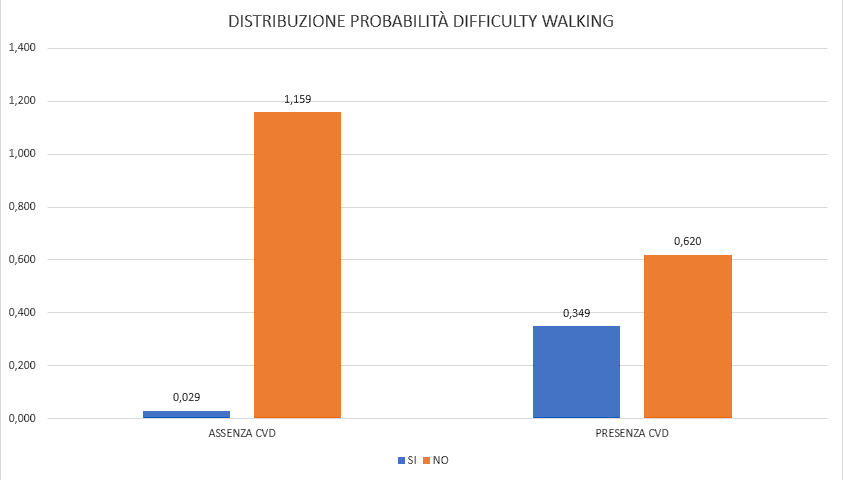
\includegraphics[width=1\linewidth]{TemplateTesi//immagini/DIFFWALK.png}
    \caption{Distribuzioni di Probabilità Difficulty Walking}
    \label{fig:dpPKIdiffwalk}
\end{figure}

\begin{figure}[H]
    \centering
    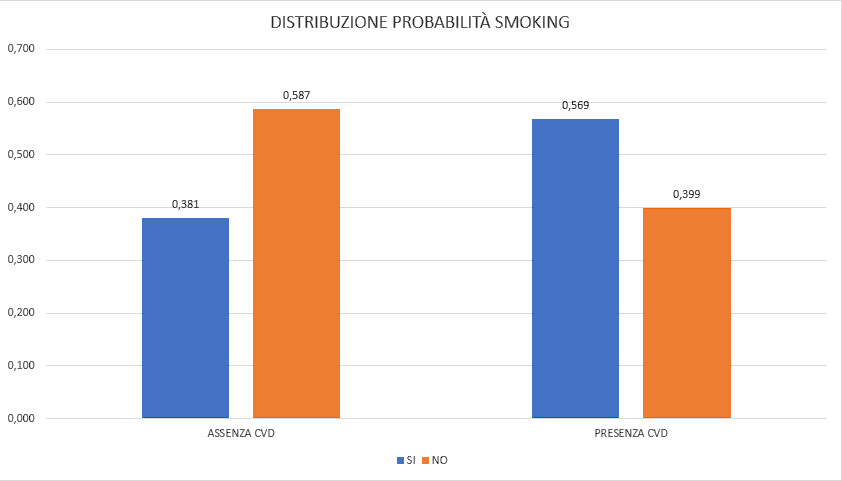
\includegraphics[width=1\linewidth]{TemplateTesi//immagini/SMOKING.png}
    \caption{Distribuzioni di Probabilità SMOKING}
    \label{fig:dpPKISMOKING}
\end{figure}

\begin{figure}[H]
    \centering
    \includegraphics[width=1\linewidth]{TemplateTesi//immagini/stroke.png}
    \caption{Distribuzioni di Probabilità  Stroke}
    \label{fig:dpPKIStroke}
\end{figure}
\begin{figure}[H]
    \centering
    \includegraphics[width=1\linewidth]{TemplateTesi//immagini/sex.png}
    \caption{Distribuzioni di Probabilità Sex}
    \label{fig:dpPKISex}
\end{figure}
Le distribuzioni in cui il caso di assenza o presenza di malattia sono molto simili, come nel caso della feature "SleepTime" del dataset PKI illustrato nella Figura \ref{fig:sleeptime}, sono state classificate come distribuzioni con un apporto poco significativo.
\begin{figure}[H]
    \centering
    \includegraphics[width=0.7\linewidth]{TemplateTesi//immagini/sleeptime.png}
    \caption{Distribuzione della feature "Sleep Time"}
    \label{fig:sleeptime}
\end{figure}


\subsubsection{Considerazioni}
\begin{flushleft}
    
Un aspetto significativo che emerge dall'analisi delle distribuzioni dei valori delle feature nei due dataset è un aumento dell'incidenza delle malattie cardiache con l'avanzamento dell'età, con un picco intorno ai 68 anni. Questo dato indica che l'età rappresenta un fattore determinante nel predisporre gli individui alla comparsa di tali patologie. 
Inoltre, si è osservata una probabilità più alta di malattie cardiache tra i fumatori. Questo risultato sottolinea l'importanza del fumo come fattore di rischio per le patologie cardiache e l'urgenza di promuovere un interruzione del tabagismo e di sensibilizzazione verso uno stile di vita sano.

Una delle correlazioni rilevanti è stata riscontrata tra il sesso maschile e l'incidenza più elevata di patologie cardiache. Ciò suggerisce che il sesso può influenzare la suscettibilità alle stesse, richiedendo un'attenzione particolare nella valutazione delle condizioni del cuore nei soggetti di sesso maschile.

Un fattore importante che è emerso è la forte correlazione tra le difficoltà deambulatorie e l'incidenza di CVD. Questo implica che i problemi di mobilità possono essere considerati come possibili indicatori di patologie in tale ambito.
In assenza di malattie cardiache, è estremamente più probabile non aver avuto un infarto. Questo collegamento è intuitivo, poiché la presenza di un infarto suggerisce un precedente danno al cuore, aumentando la probabilità di sviluppare malattie cardiache, è stato quindi importante trovare tale riscontro nei dati.

Infine, come era prevedibile, l'attività fisica contribuisce alla riduzione dell'insorgenza di tali problematiche. Questo sottolinea l'importanza dell'esercizio fisico regolare e dell'adozione di uno stile di vita attivo per la prevenzione delle CVD.
\end{flushleft}


\subsection{Analisi dei Coefficienti di Correlazione}

Si riportano per i dataset PKI e HDD
le heatmap dei coefficienti di correlazione generate




%\subsubsection{HeatMap Personal Key Indicator of Heart Disease}

\begin{figure}[H]
    \centering
    \includegraphics[width=1\linewidth]{TemplateTesi//immagini/heatmappki2.png}
    \caption{HeatMap dei coefficienti di correlazione di PKI}
    \label{fig:corrPKI}
\end{figure}


\begin{figure}[H]
    \centering
    \includegraphics[width=1.1\linewidth]{TemplateTesi//immagini/heatmapHDD.png}
    \caption{HeatMap dei coefficienti di correlazione di HDD }
    \label{fig:corrHDD}
\end{figure}




%\subsubsection{Considerazioni}
In generale, sebbene non siano stati riscontrati coefficienti di correlazione estremamente alti, i risultati sotto riportati sono comunque significativi e offrono un'importante rappresentazione delle relazioni tra le variabili considerate nei dataset. 
\begin{flushleft}
    
\newline
\textbf{PKI}
\newline
Uno dei risultati significativi emersi dai risultati in figura \ref{fig:corrPKI} è la correlazione  tra la difficoltà nel camminare (Difficulty walking) e la salute generica(Generic Health). Questo implica che vi sia una connessione rilevante tra l'abilità motoria di una persona e il suo stato di salute generale. Tale risultato potrebbe indicare l'importanza di monitorare attentamente la difficoltà nel camminare al fine di valutare e intervenire  per migliorare la propria salute generale.

Inoltre, risulta una correlazione tra la salute fisica (Physical Health) e la salute generale (Generic Health). Questo suggerisce che il benessere fisico di una persona può influire significativamente sulla sua salute generica.

Infine, si è  osservato una correlazione tra la salute fisica (Physical Health) e la difficoltà nel camminare (Difficulty walking). Questo risultato mette in evidenza come il livello di benessere fisico influenzi le capacità deambulatorie delle persone. L'identificazione di tale relazione potrebbe avere implicazioni nella progettazione della riabilitazione.
\newline
\textbf{HDD}
\newline
Uno dei risultati più significativi in figura \ref{fig:corrHDD} riguarda la buona correlazione tra St slope e St depression. 
È ragionevole riconoscere questa connessione in quanto entrambe le caratteristiche sono strettamente legate all'analisi clinica del tratto ST \cite{stsegment}dell'elettrocardiogramma.

È stata osservata una correlazione tra la ST depression e la presenza di malattie cardiache (Heart Disease). Ciò suggerisce che la depressione del tratto ST potrebbe essere un fattore importante nella valutazione della presenza o dello sviluppo di malattie cardiache. 

Inoltre, si riscontra una correlazione  tra la tipologia di dolore toracico (Chest Pain Type) e la presenza di CVD. Questo suggerisce che il tipo di dolore toracico riportato da un individuo può essere indicativo della presenza o dello sviluppo di problematiche al cuore.

Altri risultati significativi includono la correlazione tra il battito cardiaco massimo raggiunto (MAX Heart Rate) e la presenza di malattie cardiache, nonché la correlazione  tra l'angina indotta dall'esercizio fisico (Exercise Angina) e il tipo di dolore toracico con queste ultime. Questi risultati sottolineano l'importanza di tali variabili nella valutazione della salute del cuore e possono fornire utili indizi per la diagnosi e la gestione delle CVD.
\end{flushleft}


\subsection{MIScore dei Datasets}
Si riportano per i due dataset principali i MiScore calcolati per varie feature.

\begin{figure}[H]
    \centering
    \includegraphics[width=1\linewidth]{TemplateTesi//immagini/Heart_Disease_Dataset_8_mi_score.png}
    \caption{MIScore calcolati per HDD}
    \label{fig:miscorehdd}
\end{figure}



\begin{figure}[H]
    \centering
    \includegraphics[width=1\linewidth]{TemplateTesi//immagini/PKI_numerical_mi_score.png}
    \caption{MIScore calcolati per PKI}
    \label{fig:miscorePKI}
\end{figure}


%\subsubsection{Considerazioni}

\textbf{PKI}
\begin{flushleft}
    
I risultati ottenuti dal grafico dei MI Score per il dataset PKI (in figura \ref{fig:miscorePKI}) hanno indicato che l'età (Age Category) si posiziona in cima alla lista delle feature più influenti per la classificazione delle CVD. Questo suggerisce che l'età può essere un fattore chiave nel determinare la presenza o l'assenza di tali patologie (In accordo con le considerazioni ottenute durante l'analisi qualitativa delle distribuzioni).


In seconda posizione nel grafico dei MI Score troviamo la salute generale (Generic Health). 
La correlazione tra la salute generale e la presenza di patologie cardiache suggerisce l'importanza di una valutazione completa delle condizioni di salute complessive per identificare  eventuali problematiche in ambito cardiovascolare.

Al terzo posto si colloca il tempo dedicato quotidianamente al sonno (Sleep Time). Questo risultato suggerisce che le abitudini e la qualità del sonno possono essere fattori rilevanti nella valutazione delle malattie cardiache, evidenziando l'importanza di uno stile di vita sano e un adeguato riposo per preservare la salute cardiovascolare \cite{sonnocvd}.
La difficoltà nel camminare (Difficulty Walking) si piazza al quarto posto nel grafico dei MI Score. Questo sviluppo sottolinea come le condizioni motorie siano legate alle malattie cardiache, suggerendo che i problemi di mobilità possono essere un segnale di allarme per ulteriori valutazioni cardiovascolari.

Le feature relative alla presenza di diabete (Diabetic) , l'etnia e genere (Sex) occupano invece posizioni meno rilevanti di quelle attese.
\newline


\textbf{HDD}
\newline
I risultati ottenuti dal grafico dei MI Score per il dataset HDD (figura \ref{fig:miscorehdd}) hanno rivelato che il colesterolo (Chol) occupa la prima posizione nella lista delle feature più influenti per la classificazione. Questo indica come i livelli di colesterolo possano essere un indicatore significativo per la valutazione delle patologie cardiovascolari, suggerendo l'importanza del monitoraggio di questo parametro nella prevenzione e riabilitazione nel contesto cardio.

Al secondo e terzo posto troviamo il battito cardiaco massimo raggiunto (Max Heart Rate) e la tipologia di dolore toracico (Chest Pain Type). Questi risultati ci forniscono dei parametri di tipo clinico da tenere di conto in fasi diagnostiche e riabilitative.

È interessante notare che l'età (Age) e il genere (Sex) occupano posizioni poco rilevanti nel grafico, nonostante la posizione prominente dell'età nel grafico precedente. 



\end{flushleft}





\subsection{Selezione feature iniziali}
\begin{flushleft}
    
Dopo aver svolto tali analisi e tratte le suddette considerazioni, sono stati combinati tali risultati per una prima selezione del set di feature da utilizzare per la creazione dei modelli.

Per identificare i primi set di feature  è stata inizialmente eseguita una cernita qualitativa delle distribuzioni delle stesse (come quelle riportate in \ref{distribuzionisub}).
Durante l'analisi manuale e qualitativa effettuata sono state selezionate le feature che sembravano avere una potenziale influenza significativa per la classificazione, basandomi anche sull'esperienza clinica della mia referente aziendale. Successivamente, sono stati confrontati i risultati di questa analisi sulle distribuzioni con quelli ottenuti dalle heatmap dei coefficienti di correlazione e dai grafici del MI Score.

Attraverso il confronto tra queste analisi, sono state individuate le feature che mostravano correlazioni o relazioni significative in tutte le analisi, andando a scegliere sia le feature che risultavano significative in tutte e tre le analisi contemporaneamente che quelle più promettenti delle singole analisi.  

Per il dataset PKI sono state quindi inizialmente scelte le seguenti features:

 \begin{lstlisting}
Chosen_Features=['Age','Sex','Smoking','PhysicalActivity','GenHealth','DiffWalking']
\end{lstlisting}

Per il dataset HDD:
\begin{lstlisting}
Chosen_Features=['Age', 'Sex', 'chest_pain_type', 'st_depression', 'st_slope', 'exercise_angina']
\end{lstlisting}


Il dataset UCI, invece, non ha volutamente ricevuto feature selection, sono state quindi selezionate tutte le feature:

\begin{lstlisting}
Chosen_Features=['Age', 'Sex', 'chest_pain_type', 'st_depression', 'st_slope', 'exercise_angina','trestbps','Cholesterol,'fasting_blood_sugar','MaxHR','exercise_angina','vessel_fluoroscopy']
\end{lstlisting}
		
\end{flushleft}

\section{Elaborazioni Successive}
\subsection{Scelta dei Modelli}
\begin{flushleft}
    
Nella presente sezione, si delinea la fase determinante della selezione del modello per la creazione del modello finale. Verranno presentati i risultati della valutazione dei modelli considerati nel contesto del nostro problema di ricerca. Sono stati scelti quattro modelli di ML (ADA,XGB,SVM,RF), ciascuno dei quali è stato addestrato e valutato mediante le tecniche illustrate nel capitolo precedente.

%\subsubsection{Risultati della Valutazione}

Di seguito, %due esempi di valutazione dei 
mostriamo i risultati ottenuti per il dataset HDD e PKI:
i valori mostrati sono stati calcolati durante la fase di esplorazione dei modelli,calcolati con solo l'utilizzo dei set di feature iniziali, e utilizzando gli iperparametri di default dei modelli.
I grafici \ref{fig:graficosceltamodello} e \ref{fig:graficosceltamodellopki}, ci mostrano i risultati ottenuti durante l'analisi.


    
    \begin{figure}[H]
        \centering
        \includegraphics[width=0.75\linewidth]{TemplateTesi//immagini/GraficoComparazioneModelli.png}
        \caption{Valori delle metriche valutate per la scelta del modello finale per HDD.}
        \label{fig:graficosceltamodello}
    \end{figure}

\begin{figure}[H]
        \centering
        \includegraphics[width=1\linewidth]{TemplateTesi//immagini/metricheinizialipki.png}
        \caption{Valori delle metriche valutate per la scelta del modello finale per PKI.}
        \label{fig:graficosceltamodellopki}
    \end{figure}
Come anticipato nel capitolo 2, e come visibile dai grafici, Random Forest raggiunge risultati più stabili e generalmente migliori . Quindi presenteremo le analisi successive usando solo questo modello.

\end{flushleft}

\subsection{Feature Selection: esempio per PKI \label{selezionesetfinali}}
\begin{flushleft}
Durante l'analisi dei dataset, sono stati condotti dei test per identificare le feature più promettenti, oltre a quelle iniziali selezionate durante la fase di EDA, andando così a creare i set di feature finali per ogni modello. A tal proposito, saranno illustrati alcuni test effettuati sulle feature del dataset PKI, che consistono in aggiungere delle nuove feature e rivalutando la performance del modello RF. Dei test simili sono stati effettuati anche su HDD. 
\newline
Inizialmente per PKI, erano state selezionate le seguenti feature:
\emph{ChosenFeatures=[Age,Sex,Smoking,PhysicalActivity,GenHealth,DiffWalking]}
\newline
Successivamente, è stata valutata l'evoluzione delle metriche aggiungendo nuove features.
\subsubsection{Aggiunta di Physical Health}

\begin{figure}[H]
    \centering
    \includegraphics[width=1\linewidth]{TemplateTesi//immagini/PHYHEALTH.png}
    \caption{Distribuzione della Feature Physical Health in PKI}
    \label{fig:PHPKIDistr}
\end{figure}
Ho calcolato lo score delle metriche per 
\newline
\emph{ChosenFeatures=[Age,Sex,Smoking,PhysicalActivity,GenHealth,DiffWalking]}
\newline
ottenendo:
\begin{lstlisting}
'test_accuracy': array([0.75085106, 0.75871825, 0.75833272, 0.75674467, 0.75738354]), 
'test_precision': array([0.72459836, 0.73654873, 0.73590252, 0.73289951, 0.7355619 ]), 
'test_recall': array([0.80928738, 0.80558547, 0.80587398, 0.80793662, 0.80370181])}
\end{lstlisting}
Dopo aver inserito tra le features scelte 'PhysicalHealth', ottenendo così 
\newline
\emph{ChosenFeatures=[Age,Sex,Smoking,PhysicalActivity,GenHealth,DiffWalking,PhysicalHealth]}

I risultati ottenuti sulle metriche sono i seguenti:

\begin{lstlisting}
'test_accuracy': array([0.77163615, 0.78540917, 0.78433216, 0.78378255, 0.78447623]), 'test_precision': array([0.75491221, 0.76111427, 0.76292158, 0.76052892, 0.76504303]), 'test_recall': array([0.8044395 , 0.83193078, 0.82504883, 0.82840453, 0.82114237])
\end{lstlisting}

Ovvero un \emph{incremento globale di circa il 2\%}


\subsubsection{Aggiunta di SleepTime}
\begin{figure}[H]
    \centering
    \includegraphics[width=0.75\linewidth]{TemplateTesi//immagini/sleeptimePKIdistr.png}
    \caption{Distribuzione della Feature 'SleepTime' in PKI}
    \label{fig:distrsleeppki}
\end{figure}

Ho calcolato lo score delle metriche per 
\newline
\emph{ChosenFeatures=[Age,Sex,Smoking,PhysicalActivity,GenHealth,DiffWalking]}
\newline
ottenendo:
\begin{lstlisting}
'test_accuracy': array([0.75085106, 0.75871825, 0.75833272, 0.75674467, 0.75738354]), 
'test_precision': array([0.72459836, 0.73654873, 0.73590252, 0.73289951, 0.7355619 ]), 
'test_recall': array([0.80928738, 0.80558547, 0.80587398, 0.80793662, 0.80370181])}
\end{lstlisting}
Dopo aver inserito tra le features scelte 'SleepTime', ottenendo così 
\newline
\emph{ChosenFeatures=[Age,Sex,Smoking,PhysicalActivity,GenHealth,DiffWalking,SleepTime]}

I risultati ottenuti sulle metriche sono i seguenti:

\begin{lstlisting}
'test_accuracy': array([0.75021448, 0.76433383, 0.7629009 , 0.76171223, 0.76186738]), 
'test_precision': array([0.73417613, 0.74445457, 0.74446236, 0.74511044, 0.74584433]), 
'test_recall': array([0.78445868, 0.80499425, 0.80061333, 0.79557154, 0.79446179])}
\end{lstlisting}

Anche in questo caso ho ottenuto un \emph{incremento globale di circa il 2\%}
\end{flushleft}


\subsection{Set di Feature Finali}
\begin{flushleft}
    
Dopo tali test sono stati creati per tutti i dataset i set di feature finali, qui riportati:

PKI:
\begin{lstlisting}
    Chosen_Features= ['Age','Sex','Smoking','PhysicalActivity','GenHealth','DiffWalking','PhysicalHealth','SleepTime']

\end{lstlisting}
HDD:
\begin{lstlisting}
Chosen_Features = ['Age', 'Sex', 'chest_pain_type', 'st_depression', 'st_slope', 'exercise_angina','Cholesterol','MaxHR']
\end{lstlisting}
    
UCI (uguali a quelli iniziali, non avendo effettuato la feature selection):

\begin{lstlisting}
Chosen_Features=['Age', 'Sex', 'chest_pain_type', 'st_depression', 'st_slope', 'exercise_angina','trestbps','Cholesterol,'fasting_blood_sugar','MaxHR','exercise_angina','vessel_fluoroscopy']
\end{lstlisting}
\end{flushleft}

\subsection{Sbilanciamento dei dataset} 
Nella seguente sezione saranno riportate le considerazioni effettuate e le tecniche utilizzate per il bilanciamento su tutti i dataset.
\newline
\textbf{PKI sbilanciato}
\begin{flushleft}
    
Nel caso di PKI, ho invididuato, come precedentemente menzionato un forte sbilanciamento  nella rappresentazione dei valori della feature target "Heart\_Disease". La classe che rappresentava l'assenza di problemi cardiaci era sovrarappresentata rispetto alla classe per la presenza. Per affrontare questo problema, ho attuato due tecniche di bilanciamento, ovvero SMOTE, per l' undersampling e ENN per l'oversampling.  

%Applicando entrambe le tecniche , sono stato in grado di ottenere un dataset  bilanciato, con una rappresentazione più equilibrata delle classi target. Questo ha fornito un set di dati più performante durante  l'addestramento e la valutazione dei modelli di ML selezionati.



Durante l'undersampling la classe maggioritaria è stata ridotta alla dimensione di quella minoritaria, invece durante oversampling la classe minoritaria è stata augmentata per raggiungere la numerosità di quella maggioritaria. I parametri con i quali sono state utilizzate tali tecniche sono "$sampling\_strategy=minority$" per SMOTE e "$n\_neighbour=3$" per ENN.
I risultati ottenuti sulle metriche saranno descritti nel paragrafo \ref{sec:risultati}.  %4.3. 
\newline
\textbf{HDD e UCI bilanciati}
\newline


Nel caso del dataset HDD e del dataset UCI, ho osservato che i dataset erano già bilanciati( come evidenziato nelle figure \ref{fig:istoHDDtarget} e \ref{fig:istoUCItarget}). Pertanto, non ho applicato  tecniche di bilanciamento, poiché i dataset stessi presentavano una rappresentazione equilibrata della classe target.



\section{Risultati finali per i modelli di classificazione }\label{sec:risultati}

Nella sezione seguente, verranno illustrate le tecniche impiegate sui tre dataset utilizzati per generare i modelli. Ogni dataset è stato sottoposto a tecniche diverse in base alle analisi presentate nelle sezioni precedenti. Per il dataset UCI abbiamo scelto di minimizzare l'insieme di tecniche usate, per osservare il comportamento del modello in questo caso. Successivamente, verranno presentate le metriche dei modelli completati. 
È fondamentale sottolineare che ogni risultato esposto in questa sezione rappresenta la media dei risultati ottenuti attraverso la cross-validation, garantendo così una buona valutazione dell'abilità di generalizzazione degli stessi.
I set di feature utilizzati durante questa fase sono quelli finali esposti in \ref{selezionesetfinali}.

Per ognuno dei 3 dataset considerati, sarà analizzato il comportamento del modello mediante la variazione del set di tecniche utilizzate. In particolare, si esaminerà l'impatto dell'esclusione di una specifica tecnica dal set completo di tecniche impiegate. Riporteremo quindi i risultati ottenuti utilizzando l'intero set di tecniche, ad eccezione di quella specifica tecnica in questione, come indicato chiaramente nelle tabelle e nei grafici (ad esempio quelli in figura \ref{fig:andamentometrichePKI} e \ref{fig:graficoandamentoPKI}).

\subsection{Tecniche Utilizzate}


\textbf{Tecniche applicate ad UCI:}
\begin{itemize}
    \item Manipolazioni (Sostituzione variabili nominali, rimozione NaN)
    \item Scaling dei Dati
\end{itemize}




\begin{figure}[H]
    \centering
    \includegraphics[width=0.75\linewidth]{TemplateTesi//immagini/graficoUCIMetriche.png}
    \caption{Grafico Dell'Andamento delle Metriche Relative al Dataset UCI}
    \label{fig:graficoandamentoUCI}
\end{figure}

I risultati ottenuti, visibili in figura \ref{fig:graficoandamentoUCI}, mostrano che l'uso dello scaling delle feature porta ad un leggero miglioramento delle metriche del modello, sebbene l'aumento sia modesto. Questo indica che l'applicazione dello scaling comunque contribuisce a una migliore normalizzazione dei dati consentendo al modello di lavorare in modo più efficace e coerente con i dati stessi.


\textbf{Tecniche applicate ad HDD:}
\begin{itemize}
    \item Feature Selection
    \item Manipolazioni (Sostituzione variabili nominali, rimozione NaN)
    \item Scaling dei Dati
    \item Rimozione deglia outlier: Zscore
\end{itemize}




\begin{figure}[H]
    \centering
    \includegraphics[width=0.75\linewidth]{TemplateTesi//immagini/graficoHDDMetriche.png}
    \caption{Grafico dell'Andamento delle Metriche Relative al Dataset HDD}
    \label{fig:graficoandamentoHDD}
\end{figure}

Anche in questo caso i risultati (in figura \ref{fig:graficoandamentoHDD}) hanno evidenziato che l'uso dello scaling delle feature porta ad un leggero miglioramento delle metriche del modello, così come il trattamento degli outlier con Z-score. Sebbene l'aumento non sia particolarmente alto singolarmente, si osserva che con l'uso di entrambe le tecniche vi è un aumento di circa 1 punto percentuale in tutte le metriche considerate. Sebbene possa sembrare un incremento modesto, specialmente in ambito clinico, rappresenta comunque un aiuto sostanzioso per il modello.

\textbf{Tecniche applicate a PKI:}
\begin{itemize}
    \item Feature Selection
    \item Manipolazioni (Sostituzione variabili nominali, rimozione NaN)
    \item Scaling dei Dati
    \item Rimozione outlier: Zscore
    \item SMOTE
    \item ENN
\end{itemize}


\begin{figure}[H]
    \centering
    \includegraphics[width=0.75\linewidth]{TemplateTesi//immagini/graficoPKIMetriche.png}
    \caption{Grafico dell'Andamento delle Metriche Relative al Dataset PKI}
    \label{fig:graficoandamentoPKI}
\end{figure}
Analogamente a quanto verificato in precedenza si nota un aumento modesto delle metriche  con il trattamento degli outlier e lo scaling.

Un nuovo aspetto emerso dalle  analisi in figura \ref{fig:graficoandamentoPKI} riguarda l'utilizzo delle tecniche di bilanciamento come SMOTE e ENN. Data la presenza di uno sbilanciamento significativo nel dataset, queste tecniche hanno avuto un impatto estremamente significativo sulle performance del modello. In particolare, si è notato che l'applicazione di SMOTE ha influenzato in modo molto elevato la metrica di recall, evidenziando l'importanza di gestire il problema dello sbilanciamento per una classificazione accurata.


\newline
\textbf{Risultati finali:}
\newline
Dopo aver esaminato l'andamento delle metriche relative ai 3 modelli, è giunto il momento di esporre i risultati finali ottenuti su questi ultimi.

Questi risultati rappresentano una valutazione delle prestazioni dei modelli sviluppati e forniscono un'indicazione del loro livello di accuratezza e affidabilità.
I risultati finali costituiscono un importante contributo a questa tesi. Questi risultati forniscono una base per ulteriori ricerche e sviluppi nel campo del progetto in cui è calato il mio lavoro.
\begin{figure}[H]
    \centering
    \includegraphics[width=0.55\linewidth]{TemplateTesi//immagini/MetricheModelliFinali.png}
    \caption{Metriche Finali Calcolate per i 3 Dataset}
    \label{fig:metrichefinali}
\end{figure}

Come evidenziato in figura \ref{fig:metrichefinali}, i punteggi delle metriche riflettono l'efficacia dei modelli costruiti.

Come prevedibile, il modello addestrato sul dataset UCI, che prevedeva meno elaborazioni, ha mostrato risultati inferiori rispetto agli altri modelli. Tuttavia, questi risultati sono comunque accettabili e non eccessivamente bassi, tenendo conto della complessità del problema e delle limitazioni sulle tecniche impiegate imposte da me.

Sono particolarmente soddisfatto dei risultati ottenuti per gli altri due modelli, i quali hanno raggiunto punteggi molto elevati nelle metriche considerate. Questo è particolarmente significativo nel contesto clinico, poiché stiamo lavorando con dati relativi ai pazienti e la precisione delle previsioni riveste un ruolo di grande importanza.

I punteggi così elevati sono a mio avviso specialmente importanti per il dataset PKI. Questo dataset, come spiegato in precedenza, si basa in gran parte su feature di tipo "personale", dove non è necessariamente richiesta la supervisione diretta di un esperto medico. Ciò si traduce in un notevole risparmio di tempo e risorse finanziarie per il settore medico, rendendo questo approccio al ML in ambito clinico a mio avviso prezioso.
\end{flushleft}

\section{XAI}
\begin{flushleft}
    
Nella seguente sezione sarà fornito un esempio di come sono state utilizzate le tecniche di Explainable Artificial Intelligence per fornire interpretazioni e spiegazioni comprensibili dei modelli creati durante il tirocinio.

Data la natura delle feature di tipo clinico utilizzate nei dataset, è di particolare importanza garantire la trasparenza sulle decisioni prese dal modello costruito.
A titolo esemplificativo, verranno illustrate le tecniche di XAI utilizzate durante l'analisi del dataset HDD, che contiene parametri clinici.

\subsection{LIME}
Utilizzando LIME, sono stato in grado di identificare le caratteristiche cliniche che hanno avuto un impatto significativo sulle decisioni prese dal modello, tale tecnica risulta di particolare interesse quando il risultato fornito riguarda un caso liminare della classificazione.
Un esempio di visualizzazione per un caso liminare  è fornito in figura \ref{fig:LimeLiminare}.

\begin{figure}[H]
    \centering
    \includegraphics[width=1\linewidth]{TemplateTesi//immagini/casoliminare.png}
    \caption{Esempio di Visualizzazione LIME per un caso liminare}
    \label{fig:LimeLiminare}
\end{figure}

L'analisi dei risultati ottenuti mediante il grafico generato da LIME ha rivelato che la feature ST slope ha avuto il maggior impatto sulla classificazione del paziente come nella classe "0" (sena malattia). Questo indica come la feature "St slope" possa essere un elemento rilevante al fine della decisione nel nostro problema di classificazione.

Si osserva come l'età e il colesterolo abbiano hanno contribuito in senso opposto rispetto alla classificazione, in contrasto con ST slope e il resto delle feature.


Le considerazioni derivate da quest'analisi offrono alla figura medica uno strumento  per un'interpretazione più approfondita dei risultati delle previsioni.
Questo può fornire inoltre una nuova prospettiva clinica e rappresentare un caso di studio per un approccio personalizzato al trattamento dei pazienti.

\subsection{Counterfactual Explanations}


Nella seguente sezione si riportano le counterfactual explanations generate per un particolare record.
Nel suddetto caso il record ( la prima riga in figura \ref{fig:exCF}), rappresenta una paziente (poiché la feature Sex=1) con un'età di 57 anni e la presenza di malattie cardiovascolari (Heart Disease=1).

\begin{figure}[H]
    \centering
    \includegraphics[width=1\linewidth]{TemplateTesi//immagini/CFexample.png}
    \caption{Esempio di Visualizzazione delle Counterfactual Explanations}
    \label{fig:exCF}
\end{figure}

Per questo esempio, nel processo di generazione delle counterfactual explanations, ho  deciso di consentire  possibili modifiche solo sulle feature specifiche di ST depression, ST slope, "exercise angina" e "max HR", mantenendo le altre feature fisse. Questa scelta è stata effettuata per fornire un esempio tecnico di come le modifiche a queste feature possono influenzare la classificazione del modello. 

È importante sottolineare che le modifiche apportate alle feature durante la creazione delle counterfactual explanations siano puramente a scopo illustrativo dal punto di vista tecnico. È fondamentale che i range di valori modificabili delle feature siano supervisionate e valutate da un esperto clinico, in base alle sue considerazioni mediche e al contesto del paziente.
 
Si riportano quindi le variazioni effettuate dalla tecnica:

Complessivamente, sono state generate 6 counterfactual explanations.  I risultati ci mostrano come sia stato suggerito di aumentare la ST depression in 4 casi su 6, indicando che un aumento della depressione del tratto ST può potenzialmente influire fortemente sulla classificazione del modello, permettendo di cambiare alla fine la classe del paziente.
La feature ST slope è stata variata solo in due delle 6 spiegazioni generate, con una diminuzione suggerita in entrambi i casi.

La feature "exercise angina" è rimasta invariato in tutte le spiegazioni, suggerendo che la presenza o l'assenza di angina indotta dall'esercizio fisico non ha influenzato la classificazione nel nostro caso specifico.
La feature "max HR" è stata variata 3 volte, con alcune spiegazioni che suggerivano un aumento e altre un decremento del battito cardiaco massimo.


\clearpage



\addcontentsline{toc}{chapter}{Conclusioni} % Capitolo non numerato
\chapter*{Conclusioni}
\label{ch:conclusioni}

\begin{flushleft}
%\section{Conclusioni}
In conclusione della mia tesi, desidero esprimere la mia soddisfazione per i risultati ottenuti e l'opportunità di immergermi nel mondo del machine learning. Questa esperienza è stata fondamentale per la mia formazione, consentendomi di acquisire conoscenza e mettere in pratica le competenze nel campo dell'intelligenza artificiale.

Durante il mio lavoro ho sviluppato 3 modelli di ML diversi.  In tutti e tre i casi, il Random Forest ha dimostrato di essere il modello più performante e stabile.
Ho avuto modo di lavorare sia con parametri clinici ( tra cui meritano menzione "ST slope","ST depression" e "chest pain type") sia con parametri personali.
Su questi è stato per me importante menzionare l'impatto che hanno avuto "Smoking" e "Sleep Time", tali risultati suggeriscono che migliorare il proprio stato di salute può anche dipendere dallo stile di vita che si adotta quotidianamente.

La possibilità di studiare e applicare metodi di XAI è stato importante per una maggiore comprensione delle dinamiche interne ai modelli, sia per me durante la costruzione,che per i clinici che  otterranno giovamento dalla maggiore chiarezza
e dalle possibilità che offre in ambito di riabilitazione.

Guardando verso il futuro, il mio tool di esplorazione dei dati è ancora in fase di sviluppo. Tuttavia, io e il team a cui è destinato siamo fiduciosi nel suo potenziale e nei possibili sviluppi che potrà offrire. L'obiettivo principale è di rendere il tool ancora più completo nel breve termine, in attesa dei dati clinici da parte degli ospedali, su cui costruire i nuovi modelli.

Un'area di interesse che non è stata menzionata durante la tesi è l'imputazione dei dati per la creazione di un dataset unico clinico, risultato del merging degli altri dataset trovati, sulla base delle loro feature comuni. 
Ho condotto dei test preliminari in questa direzione, esplorando metodi di imputazione per gestire i dati mancanti e garantire la coerenza e l'affidabilità del dataset. 
Tuttavia i risultati non hanno suggerito la percorribilità di questo percorso.

In conclusione, sono entusiasta dei risultati ottenuti e sono grato per l'opportunità di immergermi nel campo del machine learning. Guardando avanti, sono estremamente contento ed entusiasta che il mio lavoro abbia contribuito, seppur in minima parte, ad un ausilio per la risoluzione di un tale problema di classificazione, e sono fiducioso che il mio lavoro possa avere un impatto significativo, sia internamente che esternamente a Dedalus, sulla vita delle altre persone.

\end{flushleft}


\appendix
\chapter{Appendice: Sviluppo di un Tool Esplorativo}
\section{Il Tool }
Nella presente appendice, verrà illustrato il tool esplorativo che è attualmente in fase di sviluppo per Dedalus.
Questo strumento mira a fornire un'interfaccia intuitiva  per esplorare i dati e condurre analisi esplorative dei dataset, fornendo dei prototipi di modelli e guidando nella creazione dei propri.

\subsection{Obiettivi e Target del Tool}
Dopo un colloquio nel quale sono stati individuati i requisiti funzionali del tool sono stati individuati i seguenti obiettivi che il suddetto tool deve raggiungere:
\begin{itemize}
    \item Rendere utenti consapevoli sulle caratteristiche di un determinato dataset

    \item Proporre diverse strade per la creazione di un modello di machine learning per problemi di classificazione binaria

    \item Generare sia report sulla qualità dei dati che diversi modelli esportabili

    \item Creazione di modalità diverse, personalizzabili in base all’esperienza dell’utente
\end{itemize}

Il target di utente principale che utilizzerà il tool, risultato anche questo del colloquio, è stato individuato essere:
\begin{itemize}
    \item Personale Medico, in grado di comprendere i risultati ma non particolarmente avvezzo al machine learning

    \item Tecnici con media comprensione delle tecniche di machine learning 
\end{itemize}
\subsection{Stato dell'Arte}
Lo sviluppo del suddetto tool è iniziato da poco, Attualmente  è capace di eseguire esplorazione dei dati e dare report sugli eventuali problemi legati al particolare dataset in input.
I risultati della fase di EDA sono visibili tramite file HTML (come mostrato nelle figure \ref{fig:datiapp}, \ref{fig:sampleapp}, \ref{fig:heatmapapp}, \ref{fig:overviewapp}), questi sono estrapolati dal tool attraverso file .json

\begin{figure}[H]
    \centering
    \includegraphics[width=0.8\linewidth]{TemplateTesi//immagini/tool1.png}
    \caption{Overview Generale fornita dall'applicativo}
    \label{fig:overviewapp}
\end{figure}
\begin{figure}
    \centering
    \includegraphics[width=0.7\linewidth]{TemplateTesi//immagini/tool2.png}
    \caption{HeatMap dei coefficienti di correlazione dell'applicativo}
    \label{fig:heatmapapp}
\end{figure}
\begin{figure}
    \centering
    \includegraphics[width=0.7\linewidth]{TemplateTesi//immagini/tool3.png}
    \caption{Esempio di dati forniti dall'applicativo per ogni feature}
    \label{fig:datiapp}
\end{figure}
\begin{figure}
    \centering
    \includegraphics[width=0.7\linewidth]{TemplateTesi//immagini/tool4.png}
    \caption{Sample Mostrati dall'applicativo}
    \label{fig:sampleapp}
\end{figure}


\bibliographystyle{plain} % We choose the "plain" reference style
\bibliography{bibliography} % Entries are in the refs.bib file
%\addbibresource{bibliography.bib}
%\printbibliography

\end{document}